\documentclass[UTF8,fontset=fandol,10pt,a4paper,landscape]{ctexart}
\usepackage[margin=18mm,headheight=16pt,headsep=5mm,footskip=9mm]{geometry}
\usepackage{amsmath,booktabs,array,xcolor,hyperref,tikz,pgfplots,fancyhdr}
\pgfplotsset{compat=1.18}
\definecolor{ink}{HTML}{20324A}
\definecolor{teal}{HTML}{008B83}
\definecolor{missing}{HTML}{D9DFE6}
\definecolor{land}{HTML}{E2E9DD}
\hypersetup{unicode=true,colorlinks=true,linkcolor=teal,urlcolor=teal,pdftitle={新加坡降雨2017--2024：探索与预测},pdfauthor={项目小组（Codex协助）}}
\ctexset{section={format=\Large\bfseries\color{teal}}}
\pagestyle{fancy}\fancyhf{}
\fancyhead[L]{\small 新加坡降雨 2017--2024 / Task 1 与 2}
\fancyhead[R]{\small 中文技术报告}
\fancyfoot[L]{\footnotesize 2026 年 10 月 14 日 / 实证分析与预测}
\fancyfoot[R]{\footnotesize\thepage}
\renewcommand{\headrulewidth}{.3pt}
\renewcommand{\arraystretch}{1.15}
\setlength{\parskip}{5pt}\setlength{\parindent}{0pt}
\pgfplotsset{reportaxis/.style={font=\footnotesize,grid=major,grid style={gray!15},axis line style={gray!60},tick style={gray!60},label style={font=\footnotesize},title style={font=\small},legend style={font=\scriptsize},/pgf/number format/1000 sep={}}}
\begin{document}
{\LARGE\bfseries\color{ink} 新加坡历史降雨：时空规律与概率预测}\par
{\large Task 1 与 2：2017--2024 年 Spark 探索与概率预测}\par
\vspace{2mm}

\textbf{小组成员。}潘禹翔（A0355687J）、侯佳成（A0353127J）、吴嘉蕊（A0262371J）。

\textbf{研究内容。}本项目利用 2017--2024 年的新加坡降雨观测数据分析时间与空间变化规律，并建立模型，预测监测站在未来 30 分钟内累计雨量超过给定阈值的概率。

\textbf{数据与方法。}使用 NEA / data.gov.sg 的八个年度数据集，源记录共 48,538,713 条，去重后 48,538,627 条，涉及 91 个站点 ID。全量清洗和聚合由 Spark 执行；跨年比较采用 21 个稳定站点，避免监测网络变化混入年度差异。

\textbf{主要结果。}全部有效五分钟区间中 97.08\% 无雨。合格日内样本的雨频高峰为新加坡时间 16:00--17:00。月度可用样本平均雨频以 11 月最高、7 月最低，但各月的可用年份及站点组成不完全相同。固定站点样本中，按观测时长归一化的雨量以 2019 年最低、2021 年最高。近距离站点的日雨量相关性总体高于远距离站点；八年不能据此推断长期气候变化。

\textbf{预测结果。}原算法比较采用 Spark MLlib Logistic、Linear SVM 及外部 Spark XGBoost 集成。最终三个 XGBoost 模型分别在 16 组完整参数网格上调参；2017--2021 年训练、2022 年选参数，再用全部 2017--2022 年重训。2023 年上半年校准，下半年选择概率管线和判别阈值。2024 年最终测试 PR-AUC 为 0.61218、0.22511、0.02118。0 mm 保留未校准概率，5 与 25 mm 使用校准概率。

\begin{center}\begin{tabular}{rrrrr}
\toprule
年份 & 雨量 / 观测24h（mm） & 雨频（\%） & 湿区间雨强（mm/5min） & 平均覆盖率（\%）\\\midrule
2017 & 6.85 & 2.85 & 0.833 & 94.6\\
2018 & 7.10 & 2.90 & 0.840 & 82.9\\
2019 & 4.81 & 1.97 & 0.841 & 94.7\\
2020 & 7.40 & 2.92 & 0.877 & 95.3\\
2021 & 7.84 & 3.04 & 0.895 & 97.8\\
2022 & 7.71 & 3.08 & 0.868 & 99.0\\
2023 & 7.52 & 3.16 & 0.824 & 95.2\\
2024 & 7.11 & 3.01 & 0.819 & 95.6\\
\bottomrule\end{tabular}\end{center}
\noindent 表中各年均使用相同的 21 个站点，站点等权。雨量指标按观测时长归一化，不能解释为官方年度累计或真实日累计。月度图和日内图的合格样本组成仍可变化。\clearpage\section*{1. 数据来源、字段与清洗}

\textbf{来源与字段。}每条记录包含 observation timestamp、update timestamp、station ID/name/device ID、经纬度、reading update timestamp、reading value、reading type、reading unit 及日期字段。本数据只有降雨相关观测，不包含气温、湿度和风等变量。API 预览只用于确认字段和年度 ID；所有天气结论来自完整文件。

\textbf{数据核对。}下载完整年度 CSV 后，将 Spark 读入的记录数与年度 API 元数据的记录数核对，并检查重复观测、时间对齐和雨量取值。

\textbf{清洗步骤。}Spark 按 Asia/Singapore 解析时间；保留有限、非负、单位为 mm、类型为预期五分钟累计、站点 ID 和时间合法且 CSV 记录有效的行。只有与五分钟网格的距离不超过两秒时才对齐，原始 epoch 同时保留；其他离网格记录排除并审计。按 station ID 与对齐时刻去重，优先保留 reading update 最新的行，再使用原始观测时刻及确定的字段顺序打破并列。年度文件合并后再次检查跨文件重复。
\begin{center}\begin{tabular}{rrrrrr}
\toprule
年份 & 源记录数 & 删除重复数 & 偏离网格超过2秒 & 负雨量数 & 站点数\\\midrule
2017 & 5,256,106 & 86 & 0 & 0 & 62\\
2018 & 4,594,246 & 0 & 0 & 0 & 56\\
2019 & 5,026,862 & 0 & 0 & 0 & 54\\
2020 & 6,334,473 & 0 & 0 & 0 & 80\\
2021 & 7,044,646 & 0 & 0 & 0 & 76\\
2022 & 7,133,230 & 0 & 0 & 0 & 72\\
2023 & 6,742,890 & 0 & 0 & 0 & 74\\
2024 & 6,406,260 & 0 & 0 & 0 & 70\\
\bottomrule\end{tabular}\end{center}

\textbf{清洗结果。}86 条重复记录全部来自 2017 年；八年数据中未发现负雨量、偏离五分钟网格超过两秒的时间戳或跨文件重复。缺失时段不计为零雨量。对超过 50 mm/5min 的读数进行额外筛查，本次没有触发该条件的记录。

\clearpage\section*{2. 指标定义与公平比较}
设站点在给定时间段内的有效观测数为 $N$，雨量为 $r_i\geq0$，有雨区间数为 $W=\sum_i\mathbf{1}(r_i>0)$，预期日历槽数为 $E$。本文使用：
\begin{align*}
\text{覆盖率} &= N/E,\qquad E=288\times\text{日历天数},\\
\text{雨频（\%）} &=100W/N,\\
\text{湿区间雨强（mm/5min）} &=\sum_i r_i/W\quad(W>0),\\
\text{雨量 / 观测24h（mm）} &=288\sum_i r_i/N.
\end{align*}
预期日历槽数显式处理闰年；低覆盖率也可能反映站点只运行了部分年份。雨强的分母仅包含有雨区间。对于单个站点和同一时间段，归一化雨量等于 $288\times\text{雨频}/100\times\text{湿区间雨强}$。分别取站点平均后，该乘积恒等式一般不再成立。归一化雨量不是官方日累计或年度累计，也不能恢复遗漏风暴。

\textbf{年度固定样本。}八年共出现 91 个站点 ID，其中 21 个同时满足：八年均有观测、每年覆盖率至少 80\%、经纬度跨度各不超过 $0.005^\circ$。其余 70 个只是不进入固定站点的跨年比较，清洗时没有删除这些站点的有效观测。21 个站点等权平均；不同分析使用的站点范围见下一页。

\textbf{月度与日内样本。}图 2、4 从这 21 个站点中进一步筛选数据完整的年月或小时组合。月度先对站点等权平均，再对可用年份等权平均；每个合格年月有 17--21 个站点，各月有 6--8 个可用年份。严格要求同站点同月份在八年均达标时，只剩 5、6、7、9、10、12 月，作为额外对照。

\textbf{空间比较。}图 1 使用 2024 年的站点，当年共 70 个，其中 56 个覆盖率至少 90\%，用于地图着色，另 14 个以灰色标记。图 5 使用固定 21 站的日累计，要求日覆盖率至少 95\%，每对至少有 365 个共同有效日期。80\%、90\%、95\% 是本项目选定的数据完整程度门槛。

\clearpage\section*{3. 计算环境与各项分析的样本范围}

\textbf{计算环境。}Task 1 使用 Apple Silicon Mac：10 个逻辑 CPU、16 GiB RAM，macOS 26.5.2 ARM64，Python 3.12.14、Java Temurin 17.0.20.1+1、Spark 3.5.8。Task 2 在 gpushare 运行，环境为 Python 3.11.10、Azul Zulu Java 17.0.20.1、Spark 3.5.8、XGBoost 3.2.0。gpushare 容器配额为 42 CPU、约 667.68 GiB RAM；完整特征的模型训练限定使用 20 个 CPU，默认 driver heap 为 6 GiB。

\textbf{Spark 配置与分工。}Task 1 与初始特征组比较采用单机双线程模式 \texttt{local[2]}。完整特征的模型比较与评价采用 \texttt{local[20]}，shuffle partitions 为 80，default parallelism 为 20。XGBoost 使用两个工作进程，每个任务配置 10 个 CPU。不使用 GPU，以低优先级串行执行各项实验。Spark DataFrame/SQL 与窗口函数用于全量清洗、时间聚合、标签和特征构造；模型训练与评价使用 Spark ML 管线。一般阶段 Java 堆为 6 GiB，进程总内存停止上限为 12 GiB；XGBoost 训练和评价的总内存上限为 40 GiB。

\textbf{分析样本。}各项分析根据比较目的采用相应的站点范围与数据完整性筛选条件，具体见下表。
\begin{center}\begin{tabular}{lll}
\toprule
分析 & 使用范围 & 筛选说明\\\midrule
图 1：2024 站点地图 & 当年 70 站中的 56 站 & 年覆盖率至少 90\%；另 14 站灰色标记\\
图 2：月度变化 & 固定 21 站的合格子集 & 每个合格年月保留 17--21 站\\
图 3：年度变化 & 同一组 21 站 & 其余 70 站不参与固定站点跨年比较\\
图 4：日内变化 & 固定 21 站的合格组合 & 年月小时组合覆盖率至少 80\%\\
图 5：距离与日雨量相关性 & 固定 21 站，210 对 & 日覆盖率至少 95\%，共同有效日至少 365\\
图 6 左：有雨时的雨量分布 & 八年全部 91 站 & 仅统计有雨五分钟区间\\
图 6 中、右：半小时超阈值与持续性 & 2024 年全部 70 站的有效观测 & 六个未来槽完整，或两个五分钟槽连续\\
\bottomrule\end{tabular}\end{center}

\textbf{清洗核对。}源记录数与 API 计数一致；删除 86 条重复记录，缺失时段不补成零。全部观测的无雨比例也使用全部 91 站，而不是仅使用 21 站。

\clearpage\section*{图 1：2024 年观测站降雨地图}

\begin{center}\begin{tikzpicture}
\begin{axis}[reportaxis,at={(0.0cm,0)},anchor=south west,width=10.7cm,height=8cm,title={降雨频率},xlabel={经度（东经）},ylabel={纬度（北纬）},xmin=103.59,xmax=104.11,ymin=1.14,ymax=1.49,xtick={103.6,103.7,103.8,103.9,104.0,104.1},scaled ticks=false,axis equal image,point meta min=1.8499486,point meta max=3.5497582,colormap/viridis,colorbar,colorbar style={ylabel={有雨五分钟区间（\%）}}]
\path[fill=land,draw=gray!60,line width=.2pt] (axis cs:103.7218714,1.2135462) -- (axis cs:103.7136853,1.2111756) -- (axis cs:103.7071836,1.2044931) -- (axis cs:103.7178159,1.2025194) -- (axis cs:103.7336516,1.2034740) -- (axis cs:103.7320316,1.2059304) -- (axis cs:103.7280932,1.2077765) -- (axis cs:103.7293708,1.2096419) -- (axis cs:103.7306401,1.2078811) -- (axis cs:103.7292099,1.2111542) -- (axis cs:103.7250955,1.2102398) -- (axis cs:103.7234225,1.2122353) -- (axis cs:103.7249692,1.2126089) -- (axis cs:103.7218714,1.2135462) -- cycle;
\path[fill=land,draw=gray!60,line width=.2pt] (axis cs:103.7620320,1.2111744) -- (axis cs:103.7586846,1.2177819) -- (axis cs:103.7576868,1.2058326) -- (axis cs:103.7603261,1.1982919) -- (axis cs:103.7598326,1.1959214) -- (axis cs:103.7641456,1.1914377) -- (axis cs:103.7602617,1.1965328) -- (axis cs:103.7661519,1.2024002) -- (axis cs:103.7750461,1.1968760) -- (axis cs:103.7743916,1.1931754) -- (axis cs:103.7711944,1.1905474) -- (axis cs:103.7680509,1.1895820) -- (axis cs:103.7649502,1.1905688) -- (axis cs:103.7676539,1.1891100) -- (axis cs:103.7702181,1.1893889) -- (axis cs:103.7746920,1.1927249) -- (axis cs:103.7757971,1.1971978) -- (axis cs:103.7809255,1.2002549) -- (axis cs:103.7811830,1.2094260) -- (axis cs:103.7767412,1.2109813) -- (axis cs:103.7689521,1.2082032) -- (axis cs:103.7620320,1.2111744) -- cycle;
\path[fill=land,draw=gray!60,line width=.2pt] (axis cs:103.8486849,1.2308515) -- (axis cs:103.8455629,1.2319805) -- (axis cs:103.8494038,1.2295376) -- (axis cs:103.8469575,1.2263895) -- (axis cs:103.8500045,1.2291408) -- (axis cs:103.8502351,1.2278215) -- (axis cs:103.8521824,1.2278965) -- (axis cs:103.8522575,1.2262500) -- (axis cs:103.8502724,1.2257929) -- (axis cs:103.8521355,1.2244850) -- (axis cs:103.8512222,1.2209995) -- (axis cs:103.8456362,1.2234323) -- (axis cs:103.8431678,1.2221753) -- (axis cs:103.8518459,1.2133951) -- (axis cs:103.8505147,1.2198074) -- (axis cs:103.8524453,1.2225870) -- (axis cs:103.8570170,1.2176462) -- (axis cs:103.8584159,1.2182431) -- (axis cs:103.8573537,1.2194981) -- (axis cs:103.8583086,1.2215575) -- (axis cs:103.8533371,1.2275506) -- (axis cs:103.8541599,1.2291208) -- (axis cs:103.8575994,1.2295976) -- (axis cs:103.8583408,1.2320265) -- (axis cs:103.8552723,1.2319299) -- (axis cs:103.8565583,1.2314090) -- (axis cs:103.8557012,1.2302183) -- (axis cs:103.8510722,1.2296501) -- (axis cs:103.8551221,1.2319407) -- (axis cs:103.8513256,1.2315290) -- (axis cs:103.8517156,1.2306119) -- (axis cs:103.8495406,1.2296934) -- (axis cs:103.8486849,1.2308515) -- cycle;
\path[fill=land,draw=gray!60,line width=.2pt] (axis cs:103.7476729,1.2373733) -- (axis cs:103.7399913,1.2350135) -- (axis cs:103.7402595,1.2325411) -- (axis cs:103.7521522,1.2297737) -- (axis cs:103.7602578,1.2254295) -- (axis cs:103.7688702,1.2248936) -- (axis cs:103.7708464,1.2273636) -- (axis cs:103.7672798,1.2300418) -- (axis cs:103.7600003,1.2309965) -- (axis cs:103.7573878,1.2366868) -- (axis cs:103.7543999,1.2343592) -- (axis cs:103.7476729,1.2373733) -- cycle;
\path[fill=land,draw=gray!60,line width=.2pt] (axis cs:103.7642004,1.2404758) -- (axis cs:103.7598506,1.2395345) -- (axis cs:103.7606730,1.2324175) -- (axis cs:103.7706812,1.2293918) -- (axis cs:103.7732518,1.2248868) -- (axis cs:103.7790706,1.2241368) -- (axis cs:103.7771103,1.2288073) -- (axis cs:103.7642004,1.2404758) -- cycle;
\path[fill=land,draw=gray!60,line width=.2pt] (axis cs:103.8092243,1.2599535) -- (axis cs:103.8065464,1.2594643) -- (axis cs:103.8095960,1.2558145) -- (axis cs:103.8111558,1.2561021) -- (axis cs:103.8198502,1.2487724) -- (axis cs:103.8214162,1.2494962) -- (axis cs:103.8271395,1.2418785) -- (axis cs:103.8285563,1.2426188) -- (axis cs:103.8303607,1.2408087) -- (axis cs:103.8298058,1.2396090) -- (axis cs:103.8329043,1.2377975) -- (axis cs:103.8397613,1.2404646) -- (axis cs:103.8409947,1.2419423) -- (axis cs:103.8394128,1.2424937) -- (axis cs:103.8407222,1.2476237) -- (axis cs:103.8419874,1.2473115) -- (axis cs:103.8415699,1.2422848) -- (axis cs:103.8482440,1.2512187) -- (axis cs:103.8458752,1.2532370) -- (axis cs:103.8422471,1.2522502) -- (axis cs:103.8410200,1.2500391) -- (axis cs:103.8416019,1.2536860) -- (axis cs:103.8271716,1.2546277) -- (axis cs:103.8182014,1.2599936) -- (axis cs:103.8145996,1.2589044) -- (axis cs:103.8092243,1.2599535) -- cycle;
\path[fill=land,draw=gray!60,line width=.2pt] (axis cs:103.8424306,1.2577463) -- (axis cs:103.8360929,1.2639018) -- (axis cs:103.8304601,1.2636316) -- (axis cs:103.8241852,1.2600970) -- (axis cs:103.8299800,1.2562194) -- (axis cs:103.8310878,1.2574185) -- (axis cs:103.8363807,1.2547801) -- (axis cs:103.8424306,1.2577463) -- cycle;
\path[fill=land,draw=gray!60,line width=.2pt] (axis cs:103.7122938,1.2918543) -- (axis cs:103.7113394,1.2966262) -- (axis cs:103.7112700,1.2917036) -- (axis cs:103.7064550,1.2924988) -- (axis cs:103.7035362,1.2903439) -- (axis cs:103.7074308,1.2852082) -- (axis cs:103.7062415,1.2846126) -- (axis cs:103.7075198,1.2802953) -- (axis cs:103.7109689,1.2778593) -- (axis cs:103.7084122,1.2753991) -- (axis cs:103.7045050,1.2782934) -- (axis cs:103.7035402,1.2815012) -- (axis cs:103.7002118,1.2849020) -- (axis cs:103.6949663,1.2797840) -- (axis cs:103.6961704,1.2778236) -- (axis cs:103.6933610,1.2760638) -- (axis cs:103.6922496,1.2770209) -- (axis cs:103.6884616,1.2723096) -- (axis cs:103.6840829,1.2763658) -- (axis cs:103.6907662,1.2829109) -- (axis cs:103.6957243,1.2902193) -- (axis cs:103.6877922,1.2905557) -- (axis cs:103.6758065,1.2845554) -- (axis cs:103.6564315,1.2709859) -- (axis cs:103.6691685,1.2453464) -- (axis cs:103.6650610,1.2426035) -- (axis cs:103.6687358,1.2348759) -- (axis cs:103.6730843,1.2343241) -- (axis cs:103.6761219,1.2279306) -- (axis cs:103.6719049,1.2235569) -- (axis cs:103.6696304,1.2283746) -- (axis cs:103.6715981,1.2232104) -- (axis cs:103.6724886,1.2226752) -- (axis cs:103.6741961,1.2229573) -- (axis cs:103.6903236,1.2400948) -- (axis cs:103.6859149,1.2577423) -- (axis cs:103.6801960,1.2629621) -- (axis cs:103.6849630,1.2683900) -- (axis cs:103.6936240,1.2605314) -- (axis cs:103.6962199,1.2509973) -- (axis cs:103.7138957,1.2587851) -- (axis cs:103.7140137,1.2601302) -- (axis cs:103.7047392,1.2654164) -- (axis cs:103.7066272,1.2687675) -- (axis cs:103.7090343,1.2676348) -- (axis cs:103.7100255,1.2695463) -- (axis cs:103.7106154,1.2668796) -- (axis cs:103.7220594,1.2608872) -- (axis cs:103.7256957,1.2648956) -- (axis cs:103.7289839,1.2650838) -- (axis cs:103.7288176,1.2671400) -- (axis cs:103.7231703,1.2687536) -- (axis cs:103.7263483,1.2716416) -- (axis cs:103.7328278,1.2691965) -- (axis cs:103.7401808,1.2730367) -- (axis cs:103.7357015,1.2781600) -- (axis cs:103.7293769,1.2809212) -- (axis cs:103.7264616,1.2841474) -- (axis cs:103.7247042,1.2894169) -- (axis cs:103.7207624,1.2912551) -- (axis cs:103.7189082,1.2898277) -- (axis cs:103.7199365,1.2913215) -- (axis cs:103.7180121,1.2919348) -- (axis cs:103.7174625,1.2906332) -- (axis cs:103.7122938,1.2918543) -- cycle;
\path[fill=land,draw=gray!60,line width=.2pt] (axis cs:103.9347848,1.4274582) -- (axis cs:103.9264553,1.4238528) -- (axis cs:103.9283554,1.4190909) -- (axis cs:103.9307089,1.4172997) -- (axis cs:103.9341981,1.4178389) -- (axis cs:103.9342492,1.4157588) -- (axis cs:103.9390356,1.4149261) -- (axis cs:103.9407791,1.4126004) -- (axis cs:103.9486000,1.4098409) -- (axis cs:103.9507941,1.4057751) -- (axis cs:103.9542260,1.4052956) -- (axis cs:103.9581645,1.3993755) -- (axis cs:103.9706674,1.4019552) -- (axis cs:103.9740223,1.4040136) -- (axis cs:103.9735180,1.4060345) -- (axis cs:103.9785241,1.4080405) -- (axis cs:103.9841158,1.4068838) -- (axis cs:103.9923787,1.4082651) -- (axis cs:103.9905172,1.4096951) -- (axis cs:103.9918896,1.4149416) -- (axis cs:103.9896761,1.4181120) -- (axis cs:103.9857025,1.4191236) -- (axis cs:103.9793108,1.4170770) -- (axis cs:103.9697473,1.4195916) -- (axis cs:103.9590472,1.4165605) -- (axis cs:103.9553897,1.4190717) -- (axis cs:103.9483697,1.4200054) -- (axis cs:103.9489322,1.4215867) -- (axis cs:103.9462272,1.4234840) -- (axis cs:103.9347848,1.4274582) -- cycle;
\path[fill=land,draw=gray!60,line width=.2pt] (axis cs:104.0564354,1.4319912) -- (axis cs:104.0523476,1.4280138) -- (axis cs:104.0427989,1.4314030) -- (axis cs:104.0409428,1.4274560) -- (axis cs:104.0374559,1.4250428) -- (axis cs:104.0287978,1.4252466) -- (axis cs:104.0305817,1.4126055) -- (axis cs:104.0271586,1.4129725) -- (axis cs:104.0251277,1.4192165) -- (axis cs:104.0210703,1.4212912) -- (axis cs:104.0163225,1.4292324) -- (axis cs:104.0142840,1.4289536) -- (axis cs:104.0096920,1.4241700) -- (axis cs:104.0091985,1.4186571) -- (axis cs:104.0120539,1.4107788) -- (axis cs:104.0139554,1.4090618) -- (axis cs:104.0234255,1.4087027) -- (axis cs:104.0275088,1.4120940) -- (axis cs:104.0302569,1.4115109) -- (axis cs:104.0283552,1.4079222) -- (axis cs:104.0301364,1.4044494) -- (axis cs:104.0288269,1.4029269) -- (axis cs:104.0256775,1.4016190) -- (axis cs:104.0155382,1.4016329) -- (axis cs:104.0185101,1.3929676) -- (axis cs:104.0236170,1.3863805) -- (axis cs:104.0267373,1.3844740) -- (axis cs:104.0198171,1.3917600) -- (axis cs:104.0162843,1.4006832) -- (axis cs:104.0196325,1.3984322) -- (axis cs:104.0272133,1.4004182) -- (axis cs:104.0315136,1.4038121) -- (axis cs:104.0348994,1.4032595) -- (axis cs:104.0354552,1.4056401) -- (axis cs:104.0351708,1.4025176) -- (axis cs:104.0380675,1.3956961) -- (axis cs:104.0402798,1.3954418) -- (axis cs:104.0471225,1.3850148) -- (axis cs:104.0457937,1.3843823) -- (axis cs:104.0513332,1.3806463) -- (axis cs:104.0527138,1.3783713) -- (axis cs:104.0519710,1.3765520) -- (axis cs:104.0534400,1.3758529) -- (axis cs:104.0551621,1.3777270) -- (axis cs:104.0788833,1.3868077) -- (axis cs:104.0834592,1.4063608) -- (axis cs:104.0870834,1.4055086) -- (axis cs:104.0881184,1.4031815) -- (axis cs:104.0877124,1.3971833) -- (axis cs:104.0798211,1.3826473) -- (axis cs:104.0757440,1.3709126) -- (axis cs:104.0743140,1.3632571) -- (axis cs:104.0748245,1.3557917) -- (axis cs:104.0837155,1.3406798) -- (axis cs:104.0836389,1.3387925) -- (axis cs:104.0821521,1.3378084) -- (axis cs:104.0809936,1.3380943) -- (axis cs:104.0721000,1.3454826) -- (axis cs:104.0803605,1.3381498) -- (axis cs:104.0826739,1.3376214) -- (axis cs:104.0839005,1.3385883) -- (axis cs:104.0842330,1.3401989) -- (axis cs:104.0754939,1.3550027) -- (axis cs:104.0745771,1.3615437) -- (axis cs:104.0755149,1.3689862) -- (axis cs:104.0787758,1.3791644) -- (axis cs:104.0876107,1.3959251) -- (axis cs:104.0884735,1.3999567) -- (axis cs:104.0882509,1.4039273) -- (axis cs:104.0875567,1.4052694) -- (axis cs:104.0864177,1.4062781) -- (axis cs:104.0837021,1.4070227) -- (axis cs:104.0856392,1.4100485) -- (axis cs:104.0804893,1.4191545) -- (axis cs:104.0694923,1.4273488) -- (axis cs:104.0564354,1.4319912) -- cycle;
\path[fill=land,draw=gray!60,line width=.2pt] (axis cs:104.0450543,1.4377270) -- (axis cs:104.0426081,1.4403440) -- (axis cs:104.0380805,1.4408589) -- (axis cs:104.0238326,1.4368690) -- (axis cs:104.0192836,1.4332652) -- (axis cs:104.0238258,1.4357786) -- (axis cs:104.0265712,1.4347315) -- (axis cs:104.0376514,1.4373409) -- (axis cs:104.0388559,1.4351089) -- (axis cs:104.0449187,1.4356701) -- (axis cs:104.0482086,1.4337372) -- (axis cs:104.0546221,1.4330547) -- (axis cs:104.0472859,1.4347453) -- (axis cs:104.0450543,1.4377270) -- cycle;
\path[fill=land,draw=gray!60,line width=.2pt] (axis cs:103.8182588,1.4708518) -- (axis cs:103.8053927,1.4697255) -- (axis cs:103.8076479,1.4656682) -- (axis cs:103.8049642,1.4695130) -- (axis cs:103.8030522,1.4690433) -- (axis cs:103.7771316,1.4511975) -- (axis cs:103.7709060,1.4485682) -- (axis cs:103.7691570,1.4519377) -- (axis cs:103.7697223,1.4491016) -- (axis cs:103.7668745,1.4452242) -- (axis cs:103.7676612,1.4429178) -- (axis cs:103.7662095,1.4412665) -- (axis cs:103.7670850,1.4436947) -- (axis cs:103.7649993,1.4437119) -- (axis cs:103.7626974,1.4378483) -- (axis cs:103.7545774,1.4385362) -- (axis cs:103.7526606,1.4377275) -- (axis cs:103.7527188,1.4357764) -- (axis cs:103.7520769,1.4373700) -- (axis cs:103.7496835,1.4367728) -- (axis cs:103.7440225,1.4402920) -- (axis cs:103.7423426,1.4388867) -- (axis cs:103.7385122,1.4388929) -- (axis cs:103.7376659,1.4405359) -- (axis cs:103.7365907,1.4387268) -- (axis cs:103.7372160,1.4427400) -- (axis cs:103.7318557,1.4475852) -- (axis cs:103.7300113,1.4476237) -- (axis cs:103.7303212,1.4495208) -- (axis cs:103.7229053,1.4480731) -- (axis cs:103.7226475,1.4506971) -- (axis cs:103.7193476,1.4510112) -- (axis cs:103.7066255,1.4459478) -- (axis cs:103.6956326,1.4348973) -- (axis cs:103.6882809,1.4329826) -- (axis cs:103.6857365,1.4303318) -- (axis cs:103.6831155,1.4310961) -- (axis cs:103.6804816,1.4287252) -- (axis cs:103.6780030,1.4290148) -- (axis cs:103.6743687,1.4250127) -- (axis cs:103.6716769,1.4153383) -- (axis cs:103.6730173,1.4139789) -- (axis cs:103.6708347,1.4134335) -- (axis cs:103.6710756,1.4115459) -- (axis cs:103.6694408,1.4098629) -- (axis cs:103.6653997,1.4090807) -- (axis cs:103.6650129,1.4070751) -- (axis cs:103.6624333,1.4056023) -- (axis cs:103.6636304,1.4022810) -- (axis cs:103.6615174,1.3887099) -- (axis cs:103.6574265,1.3843114) -- (axis cs:103.6529800,1.3731525) -- (axis cs:103.6511133,1.3744640) -- (axis cs:103.6512697,1.3728335) -- (axis cs:103.6493014,1.3722583) -- (axis cs:103.6437619,1.3602143) -- (axis cs:103.6405957,1.3578450) -- (axis cs:103.6382792,1.3503882) -- (axis cs:103.6368028,1.3516427) -- (axis cs:103.6342209,1.3491005) -- (axis cs:103.6347014,1.3461831) -- (axis cs:103.6364706,1.3456102) -- (axis cs:103.6356485,1.3435165) -- (axis cs:103.6343676,1.3446189) -- (axis cs:103.6355865,1.3434299) -- (axis cs:103.6341661,1.3419075) -- (axis cs:103.6339614,1.3444615) -- (axis cs:103.6331867,1.3427146) -- (axis cs:103.6347608,1.3407358) -- (axis cs:103.6181088,1.2970886) -- (axis cs:103.6174833,1.2935735) -- (axis cs:103.6209090,1.2879076) -- (axis cs:103.6200196,1.2835196) -- (axis cs:103.6173097,1.2793141) -- (axis cs:103.6121369,1.2766392) -- (axis cs:103.6060390,1.2626124) -- (axis cs:103.6068705,1.2618638) -- (axis cs:103.6100054,1.2681708) -- (axis cs:103.6138313,1.2676795) -- (axis cs:103.6128858,1.2652678) -- (axis cs:103.6140041,1.2556897) -- (axis cs:103.6121941,1.2559461) -- (axis cs:103.6119779,1.2530555) -- (axis cs:103.6082329,1.2521227) -- (axis cs:103.6089237,1.2463372) -- (axis cs:103.6120770,1.2463400) -- (axis cs:103.6125468,1.2452612) -- (axis cs:103.6107272,1.2437509) -- (axis cs:103.6053499,1.2439697) -- (axis cs:103.6057232,1.2409921) -- (axis cs:103.6113573,1.2412103) -- (axis cs:103.6121061,1.2373263) -- (axis cs:103.6161606,1.2371965) -- (axis cs:103.6183578,1.2320725) -- (axis cs:103.6178203,1.2272264) -- (axis cs:103.6099411,1.2220852) -- (axis cs:103.6088671,1.2196085) -- (axis cs:103.6066591,1.2211520) -- (axis cs:103.6064638,1.2248430) -- (axis cs:103.6065411,1.2202542) -- (axis cs:103.6426458,1.2101274) -- (axis cs:103.6442068,1.2115390) -- (axis cs:103.6435073,1.2123360) -- (axis cs:103.6427895,1.2108311) -- (axis cs:103.6411148,1.2108740) -- (axis cs:103.6104088,1.2195195) -- (axis cs:103.6115708,1.2222890) -- (axis cs:103.6144933,1.2227057) -- (axis cs:103.6190107,1.2274082) -- (axis cs:103.6194254,1.2295819) -- (axis cs:103.6175070,1.2362590) -- (axis cs:103.6216838,1.2383153) -- (axis cs:103.6154729,1.2515848) -- (axis cs:103.6154707,1.2543178) -- (axis cs:103.6290759,1.2608641) -- (axis cs:103.6217460,1.2579412) -- (axis cs:103.6215926,1.2617747) -- (axis cs:103.6386525,1.2701036) -- (axis cs:103.6389776,1.2661081) -- (axis cs:103.6324030,1.2630662) -- (axis cs:103.6394261,1.2658035) -- (axis cs:103.6404044,1.2790737) -- (axis cs:103.6471602,1.2793465) -- (axis cs:103.6500050,1.2825393) -- (axis cs:103.6498825,1.2854139) -- (axis cs:103.6351888,1.3109266) -- (axis cs:103.6376362,1.3164053) -- (axis cs:103.6401457,1.3139256) -- (axis cs:103.6396284,1.3124489) -- (axis cs:103.6404806,1.3133562) -- (axis cs:103.6432811,1.3113296) -- (axis cs:103.6461014,1.3136691) -- (axis cs:103.6453654,1.3147587) -- (axis cs:103.6463112,1.3138842) -- (axis cs:103.6496585,1.3173514) -- (axis cs:103.6517879,1.3156879) -- (axis cs:103.6461727,1.3089633) -- (axis cs:103.6497890,1.3052323) -- (axis cs:103.6489539,1.3038054) -- (axis cs:103.6540343,1.3102113) -- (axis cs:103.6570286,1.3111274) -- (axis cs:103.6574369,1.3099816) -- (axis cs:103.6540041,1.3064885) -- (axis cs:103.6547980,1.3057262) -- (axis cs:103.6537672,1.3062204) -- (axis cs:103.6498210,1.3016827) -- (axis cs:103.6508446,1.3004613) -- (axis cs:103.6533560,1.3025933) -- (axis cs:103.6512250,1.2999916) -- (axis cs:103.6538227,1.3013019) -- (axis cs:103.6517678,1.2993374) -- (axis cs:103.6537510,1.3010146) -- (axis cs:103.6549282,1.2996593) -- (axis cs:103.6530519,1.2978329) -- (axis cs:103.6551805,1.2996310) -- (axis cs:103.6573391,1.2979103) -- (axis cs:103.6549011,1.2956166) -- (axis cs:103.6582254,1.2972388) -- (axis cs:103.6587850,1.2953365) -- (axis cs:103.6647575,1.2918636) -- (axis cs:103.6664408,1.2888460) -- (axis cs:103.6644960,1.2869247) -- (axis cs:103.6743803,1.2952635) -- (axis cs:103.6695020,1.3004336) -- (axis cs:103.6687381,1.3062925) -- (axis cs:103.6727046,1.3067940) -- (axis cs:103.6732136,1.3022238) -- (axis cs:103.6784339,1.2965888) -- (axis cs:103.6793691,1.2971788) -- (axis cs:103.6778311,1.2996652) -- (axis cs:103.6801249,1.2971736) -- (axis cs:103.6819040,1.2979865) -- (axis cs:103.6799362,1.3074632) -- (axis cs:103.6813899,1.3100089) -- (axis cs:103.6830343,1.3087891) -- (axis cs:103.6838606,1.2990801) -- (axis cs:103.6937884,1.3006493) -- (axis cs:103.6936115,1.3051766) -- (axis cs:103.6951240,1.3078075) -- (axis cs:103.6975186,1.3079392) -- (axis cs:103.6989904,1.3052733) -- (axis cs:103.7022863,1.3040062) -- (axis cs:103.7023992,1.3018237) -- (axis cs:103.7086886,1.3020480) -- (axis cs:103.7083835,1.3076134) -- (axis cs:103.7099572,1.3070171) -- (axis cs:103.7108258,1.3084149) -- (axis cs:103.7113395,1.2971629) -- (axis cs:103.7118883,1.2995865) -- (axis cs:103.7219279,1.2994621) -- (axis cs:103.7146266,1.3065352) -- (axis cs:103.7125573,1.3065835) -- (axis cs:103.7127174,1.3088684) -- (axis cs:103.7158417,1.3084267) -- (axis cs:103.7279367,1.3001075) -- (axis cs:103.7297772,1.3015932) -- (axis cs:103.7408521,1.2988015) -- (axis cs:103.7432117,1.3011478) -- (axis cs:103.7434282,1.2998111) -- (axis cs:103.7447614,1.3008186) -- (axis cs:103.7442093,1.2980363) -- (axis cs:103.7492007,1.2962988) -- (axis cs:103.7557489,1.2972886) -- (axis cs:103.7577412,1.3000673) -- (axis cs:103.7630421,1.2946161) -- (axis cs:103.7607166,1.2906021) -- (axis cs:103.7723383,1.2836930) -- (axis cs:103.7691344,1.2783691) -- (axis cs:103.7564771,1.2858293) -- (axis cs:103.7530224,1.2853155) -- (axis cs:103.7501846,1.2805019) -- (axis cs:103.7706766,1.2682258) -- (axis cs:103.7782058,1.2809173) -- (axis cs:103.7805823,1.2795141) -- (axis cs:103.7799596,1.2783461) -- (axis cs:103.7870605,1.2737594) -- (axis cs:103.7785642,1.2592010) -- (axis cs:103.7855063,1.2550200) -- (axis cs:103.7953085,1.2715722) -- (axis cs:103.7955723,1.2700867) -- (axis cs:103.7973420,1.2700456) -- (axis cs:103.8051473,1.2622774) -- (axis cs:103.8067358,1.2662291) -- (axis cs:103.8100922,1.2646416) -- (axis cs:103.8124604,1.2664141) -- (axis cs:103.8160516,1.2637829) -- (axis cs:103.8175506,1.2666830) -- (axis cs:103.8167869,1.2637038) -- (axis cs:103.8194715,1.2639086) -- (axis cs:103.8197099,1.2622559) -- (axis cs:103.8176424,1.2619600) -- (axis cs:103.8198650,1.2619386) -- (axis cs:103.8199064,1.2630808) -- (axis cs:103.8244200,1.2630748) -- (axis cs:103.8321670,1.2674278) -- (axis cs:103.8396526,1.2676267) -- (axis cs:103.8457821,1.2616611) -- (axis cs:103.8467730,1.2627421) -- (axis cs:103.8444309,1.2656247) -- (axis cs:103.8456794,1.2668761) -- (axis cs:103.8512255,1.2606747) -- (axis cs:103.8516078,1.2728398) -- (axis cs:103.8584945,1.2693503) -- (axis cs:103.8579787,1.2683336) -- (axis cs:103.8608496,1.2647333) -- (axis cs:103.8617123,1.2653498) -- (axis cs:103.8599603,1.2677976) -- (axis cs:103.8716769,1.2768781) -- (axis cs:103.8714562,1.2805550) -- (axis cs:103.8737178,1.2822201) -- (axis cs:103.8757276,1.2807170) -- (axis cs:103.8776890,1.2807350) -- (axis cs:103.8758917,1.2807729) -- (axis cs:103.8797504,1.2833276) -- (axis cs:103.8796729,1.2843651) -- (axis cs:103.8936756,1.2935206) -- (axis cs:103.8963751,1.2931770) -- (axis cs:103.9007930,1.2960860) -- (axis cs:103.9165583,1.3013812) -- (axis cs:103.9321877,1.3056014) -- (axis cs:103.9335464,1.3048712) -- (axis cs:103.9485395,1.3105790) -- (axis cs:103.9557581,1.3112303) -- (axis cs:103.9631165,1.3146177) -- (axis cs:103.9757511,1.3163696) -- (axis cs:103.9767675,1.3151917) -- (axis cs:103.9834673,1.3168347) -- (axis cs:103.9852381,1.3133709) -- (axis cs:103.9839171,1.3120678) -- (axis cs:103.9906944,1.3140089) -- (axis cs:104.0006331,1.3103307) -- (axis cs:104.0114272,1.3152807) -- (axis cs:104.0224125,1.3154343) -- (axis cs:104.0229163,1.3199628) -- (axis cs:104.0287502,1.3201058) -- (axis cs:104.0288982,1.3158118) -- (axis cs:104.0327311,1.3161314) -- (axis cs:104.0335984,1.3174026) -- (axis cs:104.0323397,1.3249192) -- (axis cs:104.0231536,1.3248948) -- (axis cs:104.0209889,1.3269507) -- (axis cs:104.0221413,1.3346203) -- (axis cs:104.0246329,1.3358125) -- (axis cs:104.0316545,1.3537211) -- (axis cs:104.0325318,1.3509476) -- (axis cs:104.0301054,1.3490751) -- (axis cs:104.0326689,1.3507934) -- (axis cs:104.0327309,1.3584039) -- (axis cs:104.0378255,1.3569563) -- (axis cs:104.0420205,1.3519602) -- (axis cs:104.0433039,1.3541415) -- (axis cs:104.0278327,1.3637475) -- (axis cs:104.0155066,1.3683283) -- (axis cs:104.0137145,1.3701687) -- (axis cs:104.0101775,1.3687146) -- (axis cs:104.0062655,1.3699572) -- (axis cs:104.0065479,1.3724714) -- (axis cs:104.0088241,1.3735765) -- (axis cs:104.0057428,1.3751740) -- (axis cs:103.9990392,1.3890380) -- (axis cs:103.9870888,1.3934326) -- (axis cs:103.9864779,1.3927176) -- (axis cs:103.9901005,1.3900550) -- (axis cs:103.9816617,1.3929900) -- (axis cs:103.9737816,1.3903800) -- (axis cs:103.9744288,1.3873270) -- (axis cs:103.9766002,1.3862741) -- (axis cs:103.9716404,1.3868183) -- (axis cs:103.9672216,1.3832887) -- (axis cs:103.9667880,1.3801998) -- (axis cs:103.9644751,1.3821290) -- (axis cs:103.9598207,1.3811390) -- (axis cs:103.9490378,1.3830880) -- (axis cs:103.9377941,1.3899507) -- (axis cs:103.9341970,1.3966828) -- (axis cs:103.9301739,1.3994603) -- (axis cs:103.9308457,1.4040196) -- (axis cs:103.9163703,1.4172481) -- (axis cs:103.9140967,1.4163367) -- (axis cs:103.9125266,1.4212252) -- (axis cs:103.9032489,1.4199306) -- (axis cs:103.8980253,1.4147270) -- (axis cs:103.8966801,1.4153418) -- (axis cs:103.8979293,1.4183101) -- (axis cs:103.8969491,1.4206060) -- (axis cs:103.8888773,1.4255754) -- (axis cs:103.8865729,1.4235974) -- (axis cs:103.8881975,1.4257500) -- (axis cs:103.8770922,1.4320010) -- (axis cs:103.8697209,1.4285682) -- (axis cs:103.8695778,1.4245748) -- (axis cs:103.8639737,1.4238589) -- (axis cs:103.8634290,1.4226914) -- (axis cs:103.8573725,1.4253534) -- (axis cs:103.8625597,1.4350457) -- (axis cs:103.8573417,1.4416513) -- (axis cs:103.8548383,1.4483195) -- (axis cs:103.8464426,1.4481606) -- (axis cs:103.8476029,1.4459637) -- (axis cs:103.8456568,1.4478619) -- (axis cs:103.8458937,1.4540789) -- (axis cs:103.8480491,1.4491261) -- (axis cs:103.8520917,1.4512969) -- (axis cs:103.8504919,1.4554899) -- (axis cs:103.8364373,1.4641319) -- (axis cs:103.8352614,1.4641570) -- (axis cs:103.8329059,1.4599476) -- (axis cs:103.8319875,1.4604881) -- (axis cs:103.8343307,1.4647354) -- (axis cs:103.8275713,1.4685888) -- (axis cs:103.8245580,1.4633250) -- (axis cs:103.8233659,1.4640054) -- (axis cs:103.8241553,1.4654385) -- (axis cs:103.8220573,1.4666180) -- (axis cs:103.8184541,1.4639199) -- (axis cs:103.8223514,1.4689723) -- (axis cs:103.8182588,1.4708518) -- cycle;
\addplot[scatter,only marks,mark=*,mark size=2.5pt,scatter src=explicit,draw=white] coordinates {(103.8334000,1.3415000)[3.4435342] (103.8271000,1.3701000)[3.1824463] (103.7853800,1.4438700)[3.0918641] (103.9625000,1.3135000)[2.5892315] (103.8492000,1.3764000)[3.2890478] (103.8365000,1.3105500)[3.0057848] (103.9104000,1.3064800)[2.5503769] (103.6184300,1.2937700)[2.8535368] (103.7540000,1.2810000)[2.9783514] (103.6790000,1.2560000)[3.0748623] (103.8666000,1.3010500)[2.7376375] (103.7224400,1.3728800)[3.2260951] (103.7671400,1.3231100)[3.2437936] (103.7702000,1.2916400)[3.1747778] (103.9583600,1.3248500)[2.7414981] (104.0031700,1.3136000)[1.8499486] (103.8447200,1.4211100)[3.1501838] (103.7690400,1.4400300)[3.1479295] (103.7571100,1.4291800)[3.2347665] (103.8097000,1.3242700)[3.2224443] (103.8828900,1.2991100)[2.5328018] (103.8889900,1.3278500)[2.7249471] (103.8533500,1.3601900)[3.2208034] (103.8552600,1.3504100)[3.2212619] (103.7506500,1.3649100)[3.2874079] (103.8764300,1.3799900)[3.1883920] (103.8979700,1.3866600)[2.8519770] (103.8908800,1.3569100)[3.0669357] (103.8236400,1.2898700)[3.0123292] (103.8026400,1.2998400)[2.9495552] (103.9840900,1.3439200)[2.4448970] (103.8038900,1.2747200)[2.9807924] (103.8038900,1.4394400)[3.2163214] (103.7007300,1.3470300)[3.3176979] (103.7219500,1.3516700)[3.2341859] (103.7644400,1.3016700)[3.0342242] (103.9826000,1.3678000)[2.8477024] (103.7100000,1.3081000)[3.5497582] (103.7556000,1.3329000)[3.1560859] (103.7896200,1.4044000)[3.2294191] (103.8878000,1.3399000)[2.9989659] (103.6816600,1.3458300)[3.2741796] (103.7768000,1.3337000)[3.1556849] (103.7603000,1.3824000)[3.3426584] (103.7363000,1.4387000)[3.4082697] (103.8050000,1.3700000)[3.3929479] (103.7815000,1.2923000)[3.1618164] (103.8125000,1.2937000)[2.9195740] (103.8906700,1.3070300)[2.7997336] (103.9092000,1.4029000)[3.0049620] (103.9444000,1.3437000)[2.9166544] (103.8482000,1.3427000)[3.2600388] (103.6616200,1.3198500)[3.2422172] (103.8191000,1.3191000)[3.2326640] (103.8692200,1.4128400)[3.2314234] (103.9528000,1.3662000)[2.7463803]};
\addplot[gray,only marks,mark=x,mark size=2.2pt] coordinates {(103.9007000,1.3524000) (103.7680000,1.1890000) (103.9673000,1.4168000) (103.8703000,1.2799000) (103.7013100,1.4385400) (103.7300000,1.3800000) (103.8461000,1.2994000) (103.8180000,1.3087400) (103.8577000,1.3214000) (103.9357400,1.3183500) (103.9350000,1.3870000) (103.8279000,1.2500000) (103.8372000,1.3004000) (103.7886000,1.2841000)};
\end{axis}
\begin{axis}[reportaxis,at={(12.8cm,0)},anchor=south west,width=10.7cm,height=8cm,title={有雨区间平均雨量},xlabel={经度（东经）},ylabel={纬度（北纬）},xmin=103.59,xmax=104.11,ymin=1.14,ymax=1.49,xtick={103.6,103.7,103.8,103.9,104.0,104.1},scaled ticks=false,axis equal image,point meta min=0.7342727,point meta max=0.9731774,colormap/hot2,colorbar,colorbar style={ylabel={mm / 湿五分钟}}]
\path[fill=land,draw=gray!60,line width=.2pt] (axis cs:103.7218714,1.2135462) -- (axis cs:103.7136853,1.2111756) -- (axis cs:103.7071836,1.2044931) -- (axis cs:103.7178159,1.2025194) -- (axis cs:103.7336516,1.2034740) -- (axis cs:103.7320316,1.2059304) -- (axis cs:103.7280932,1.2077765) -- (axis cs:103.7293708,1.2096419) -- (axis cs:103.7306401,1.2078811) -- (axis cs:103.7292099,1.2111542) -- (axis cs:103.7250955,1.2102398) -- (axis cs:103.7234225,1.2122353) -- (axis cs:103.7249692,1.2126089) -- (axis cs:103.7218714,1.2135462) -- cycle;
\path[fill=land,draw=gray!60,line width=.2pt] (axis cs:103.7620320,1.2111744) -- (axis cs:103.7586846,1.2177819) -- (axis cs:103.7576868,1.2058326) -- (axis cs:103.7603261,1.1982919) -- (axis cs:103.7598326,1.1959214) -- (axis cs:103.7641456,1.1914377) -- (axis cs:103.7602617,1.1965328) -- (axis cs:103.7661519,1.2024002) -- (axis cs:103.7750461,1.1968760) -- (axis cs:103.7743916,1.1931754) -- (axis cs:103.7711944,1.1905474) -- (axis cs:103.7680509,1.1895820) -- (axis cs:103.7649502,1.1905688) -- (axis cs:103.7676539,1.1891100) -- (axis cs:103.7702181,1.1893889) -- (axis cs:103.7746920,1.1927249) -- (axis cs:103.7757971,1.1971978) -- (axis cs:103.7809255,1.2002549) -- (axis cs:103.7811830,1.2094260) -- (axis cs:103.7767412,1.2109813) -- (axis cs:103.7689521,1.2082032) -- (axis cs:103.7620320,1.2111744) -- cycle;
\path[fill=land,draw=gray!60,line width=.2pt] (axis cs:103.8486849,1.2308515) -- (axis cs:103.8455629,1.2319805) -- (axis cs:103.8494038,1.2295376) -- (axis cs:103.8469575,1.2263895) -- (axis cs:103.8500045,1.2291408) -- (axis cs:103.8502351,1.2278215) -- (axis cs:103.8521824,1.2278965) -- (axis cs:103.8522575,1.2262500) -- (axis cs:103.8502724,1.2257929) -- (axis cs:103.8521355,1.2244850) -- (axis cs:103.8512222,1.2209995) -- (axis cs:103.8456362,1.2234323) -- (axis cs:103.8431678,1.2221753) -- (axis cs:103.8518459,1.2133951) -- (axis cs:103.8505147,1.2198074) -- (axis cs:103.8524453,1.2225870) -- (axis cs:103.8570170,1.2176462) -- (axis cs:103.8584159,1.2182431) -- (axis cs:103.8573537,1.2194981) -- (axis cs:103.8583086,1.2215575) -- (axis cs:103.8533371,1.2275506) -- (axis cs:103.8541599,1.2291208) -- (axis cs:103.8575994,1.2295976) -- (axis cs:103.8583408,1.2320265) -- (axis cs:103.8552723,1.2319299) -- (axis cs:103.8565583,1.2314090) -- (axis cs:103.8557012,1.2302183) -- (axis cs:103.8510722,1.2296501) -- (axis cs:103.8551221,1.2319407) -- (axis cs:103.8513256,1.2315290) -- (axis cs:103.8517156,1.2306119) -- (axis cs:103.8495406,1.2296934) -- (axis cs:103.8486849,1.2308515) -- cycle;
\path[fill=land,draw=gray!60,line width=.2pt] (axis cs:103.7476729,1.2373733) -- (axis cs:103.7399913,1.2350135) -- (axis cs:103.7402595,1.2325411) -- (axis cs:103.7521522,1.2297737) -- (axis cs:103.7602578,1.2254295) -- (axis cs:103.7688702,1.2248936) -- (axis cs:103.7708464,1.2273636) -- (axis cs:103.7672798,1.2300418) -- (axis cs:103.7600003,1.2309965) -- (axis cs:103.7573878,1.2366868) -- (axis cs:103.7543999,1.2343592) -- (axis cs:103.7476729,1.2373733) -- cycle;
\path[fill=land,draw=gray!60,line width=.2pt] (axis cs:103.7642004,1.2404758) -- (axis cs:103.7598506,1.2395345) -- (axis cs:103.7606730,1.2324175) -- (axis cs:103.7706812,1.2293918) -- (axis cs:103.7732518,1.2248868) -- (axis cs:103.7790706,1.2241368) -- (axis cs:103.7771103,1.2288073) -- (axis cs:103.7642004,1.2404758) -- cycle;
\path[fill=land,draw=gray!60,line width=.2pt] (axis cs:103.8092243,1.2599535) -- (axis cs:103.8065464,1.2594643) -- (axis cs:103.8095960,1.2558145) -- (axis cs:103.8111558,1.2561021) -- (axis cs:103.8198502,1.2487724) -- (axis cs:103.8214162,1.2494962) -- (axis cs:103.8271395,1.2418785) -- (axis cs:103.8285563,1.2426188) -- (axis cs:103.8303607,1.2408087) -- (axis cs:103.8298058,1.2396090) -- (axis cs:103.8329043,1.2377975) -- (axis cs:103.8397613,1.2404646) -- (axis cs:103.8409947,1.2419423) -- (axis cs:103.8394128,1.2424937) -- (axis cs:103.8407222,1.2476237) -- (axis cs:103.8419874,1.2473115) -- (axis cs:103.8415699,1.2422848) -- (axis cs:103.8482440,1.2512187) -- (axis cs:103.8458752,1.2532370) -- (axis cs:103.8422471,1.2522502) -- (axis cs:103.8410200,1.2500391) -- (axis cs:103.8416019,1.2536860) -- (axis cs:103.8271716,1.2546277) -- (axis cs:103.8182014,1.2599936) -- (axis cs:103.8145996,1.2589044) -- (axis cs:103.8092243,1.2599535) -- cycle;
\path[fill=land,draw=gray!60,line width=.2pt] (axis cs:103.8424306,1.2577463) -- (axis cs:103.8360929,1.2639018) -- (axis cs:103.8304601,1.2636316) -- (axis cs:103.8241852,1.2600970) -- (axis cs:103.8299800,1.2562194) -- (axis cs:103.8310878,1.2574185) -- (axis cs:103.8363807,1.2547801) -- (axis cs:103.8424306,1.2577463) -- cycle;
\path[fill=land,draw=gray!60,line width=.2pt] (axis cs:103.7122938,1.2918543) -- (axis cs:103.7113394,1.2966262) -- (axis cs:103.7112700,1.2917036) -- (axis cs:103.7064550,1.2924988) -- (axis cs:103.7035362,1.2903439) -- (axis cs:103.7074308,1.2852082) -- (axis cs:103.7062415,1.2846126) -- (axis cs:103.7075198,1.2802953) -- (axis cs:103.7109689,1.2778593) -- (axis cs:103.7084122,1.2753991) -- (axis cs:103.7045050,1.2782934) -- (axis cs:103.7035402,1.2815012) -- (axis cs:103.7002118,1.2849020) -- (axis cs:103.6949663,1.2797840) -- (axis cs:103.6961704,1.2778236) -- (axis cs:103.6933610,1.2760638) -- (axis cs:103.6922496,1.2770209) -- (axis cs:103.6884616,1.2723096) -- (axis cs:103.6840829,1.2763658) -- (axis cs:103.6907662,1.2829109) -- (axis cs:103.6957243,1.2902193) -- (axis cs:103.6877922,1.2905557) -- (axis cs:103.6758065,1.2845554) -- (axis cs:103.6564315,1.2709859) -- (axis cs:103.6691685,1.2453464) -- (axis cs:103.6650610,1.2426035) -- (axis cs:103.6687358,1.2348759) -- (axis cs:103.6730843,1.2343241) -- (axis cs:103.6761219,1.2279306) -- (axis cs:103.6719049,1.2235569) -- (axis cs:103.6696304,1.2283746) -- (axis cs:103.6715981,1.2232104) -- (axis cs:103.6724886,1.2226752) -- (axis cs:103.6741961,1.2229573) -- (axis cs:103.6903236,1.2400948) -- (axis cs:103.6859149,1.2577423) -- (axis cs:103.6801960,1.2629621) -- (axis cs:103.6849630,1.2683900) -- (axis cs:103.6936240,1.2605314) -- (axis cs:103.6962199,1.2509973) -- (axis cs:103.7138957,1.2587851) -- (axis cs:103.7140137,1.2601302) -- (axis cs:103.7047392,1.2654164) -- (axis cs:103.7066272,1.2687675) -- (axis cs:103.7090343,1.2676348) -- (axis cs:103.7100255,1.2695463) -- (axis cs:103.7106154,1.2668796) -- (axis cs:103.7220594,1.2608872) -- (axis cs:103.7256957,1.2648956) -- (axis cs:103.7289839,1.2650838) -- (axis cs:103.7288176,1.2671400) -- (axis cs:103.7231703,1.2687536) -- (axis cs:103.7263483,1.2716416) -- (axis cs:103.7328278,1.2691965) -- (axis cs:103.7401808,1.2730367) -- (axis cs:103.7357015,1.2781600) -- (axis cs:103.7293769,1.2809212) -- (axis cs:103.7264616,1.2841474) -- (axis cs:103.7247042,1.2894169) -- (axis cs:103.7207624,1.2912551) -- (axis cs:103.7189082,1.2898277) -- (axis cs:103.7199365,1.2913215) -- (axis cs:103.7180121,1.2919348) -- (axis cs:103.7174625,1.2906332) -- (axis cs:103.7122938,1.2918543) -- cycle;
\path[fill=land,draw=gray!60,line width=.2pt] (axis cs:103.9347848,1.4274582) -- (axis cs:103.9264553,1.4238528) -- (axis cs:103.9283554,1.4190909) -- (axis cs:103.9307089,1.4172997) -- (axis cs:103.9341981,1.4178389) -- (axis cs:103.9342492,1.4157588) -- (axis cs:103.9390356,1.4149261) -- (axis cs:103.9407791,1.4126004) -- (axis cs:103.9486000,1.4098409) -- (axis cs:103.9507941,1.4057751) -- (axis cs:103.9542260,1.4052956) -- (axis cs:103.9581645,1.3993755) -- (axis cs:103.9706674,1.4019552) -- (axis cs:103.9740223,1.4040136) -- (axis cs:103.9735180,1.4060345) -- (axis cs:103.9785241,1.4080405) -- (axis cs:103.9841158,1.4068838) -- (axis cs:103.9923787,1.4082651) -- (axis cs:103.9905172,1.4096951) -- (axis cs:103.9918896,1.4149416) -- (axis cs:103.9896761,1.4181120) -- (axis cs:103.9857025,1.4191236) -- (axis cs:103.9793108,1.4170770) -- (axis cs:103.9697473,1.4195916) -- (axis cs:103.9590472,1.4165605) -- (axis cs:103.9553897,1.4190717) -- (axis cs:103.9483697,1.4200054) -- (axis cs:103.9489322,1.4215867) -- (axis cs:103.9462272,1.4234840) -- (axis cs:103.9347848,1.4274582) -- cycle;
\path[fill=land,draw=gray!60,line width=.2pt] (axis cs:104.0564354,1.4319912) -- (axis cs:104.0523476,1.4280138) -- (axis cs:104.0427989,1.4314030) -- (axis cs:104.0409428,1.4274560) -- (axis cs:104.0374559,1.4250428) -- (axis cs:104.0287978,1.4252466) -- (axis cs:104.0305817,1.4126055) -- (axis cs:104.0271586,1.4129725) -- (axis cs:104.0251277,1.4192165) -- (axis cs:104.0210703,1.4212912) -- (axis cs:104.0163225,1.4292324) -- (axis cs:104.0142840,1.4289536) -- (axis cs:104.0096920,1.4241700) -- (axis cs:104.0091985,1.4186571) -- (axis cs:104.0120539,1.4107788) -- (axis cs:104.0139554,1.4090618) -- (axis cs:104.0234255,1.4087027) -- (axis cs:104.0275088,1.4120940) -- (axis cs:104.0302569,1.4115109) -- (axis cs:104.0283552,1.4079222) -- (axis cs:104.0301364,1.4044494) -- (axis cs:104.0288269,1.4029269) -- (axis cs:104.0256775,1.4016190) -- (axis cs:104.0155382,1.4016329) -- (axis cs:104.0185101,1.3929676) -- (axis cs:104.0236170,1.3863805) -- (axis cs:104.0267373,1.3844740) -- (axis cs:104.0198171,1.3917600) -- (axis cs:104.0162843,1.4006832) -- (axis cs:104.0196325,1.3984322) -- (axis cs:104.0272133,1.4004182) -- (axis cs:104.0315136,1.4038121) -- (axis cs:104.0348994,1.4032595) -- (axis cs:104.0354552,1.4056401) -- (axis cs:104.0351708,1.4025176) -- (axis cs:104.0380675,1.3956961) -- (axis cs:104.0402798,1.3954418) -- (axis cs:104.0471225,1.3850148) -- (axis cs:104.0457937,1.3843823) -- (axis cs:104.0513332,1.3806463) -- (axis cs:104.0527138,1.3783713) -- (axis cs:104.0519710,1.3765520) -- (axis cs:104.0534400,1.3758529) -- (axis cs:104.0551621,1.3777270) -- (axis cs:104.0788833,1.3868077) -- (axis cs:104.0834592,1.4063608) -- (axis cs:104.0870834,1.4055086) -- (axis cs:104.0881184,1.4031815) -- (axis cs:104.0877124,1.3971833) -- (axis cs:104.0798211,1.3826473) -- (axis cs:104.0757440,1.3709126) -- (axis cs:104.0743140,1.3632571) -- (axis cs:104.0748245,1.3557917) -- (axis cs:104.0837155,1.3406798) -- (axis cs:104.0836389,1.3387925) -- (axis cs:104.0821521,1.3378084) -- (axis cs:104.0809936,1.3380943) -- (axis cs:104.0721000,1.3454826) -- (axis cs:104.0803605,1.3381498) -- (axis cs:104.0826739,1.3376214) -- (axis cs:104.0839005,1.3385883) -- (axis cs:104.0842330,1.3401989) -- (axis cs:104.0754939,1.3550027) -- (axis cs:104.0745771,1.3615437) -- (axis cs:104.0755149,1.3689862) -- (axis cs:104.0787758,1.3791644) -- (axis cs:104.0876107,1.3959251) -- (axis cs:104.0884735,1.3999567) -- (axis cs:104.0882509,1.4039273) -- (axis cs:104.0875567,1.4052694) -- (axis cs:104.0864177,1.4062781) -- (axis cs:104.0837021,1.4070227) -- (axis cs:104.0856392,1.4100485) -- (axis cs:104.0804893,1.4191545) -- (axis cs:104.0694923,1.4273488) -- (axis cs:104.0564354,1.4319912) -- cycle;
\path[fill=land,draw=gray!60,line width=.2pt] (axis cs:104.0450543,1.4377270) -- (axis cs:104.0426081,1.4403440) -- (axis cs:104.0380805,1.4408589) -- (axis cs:104.0238326,1.4368690) -- (axis cs:104.0192836,1.4332652) -- (axis cs:104.0238258,1.4357786) -- (axis cs:104.0265712,1.4347315) -- (axis cs:104.0376514,1.4373409) -- (axis cs:104.0388559,1.4351089) -- (axis cs:104.0449187,1.4356701) -- (axis cs:104.0482086,1.4337372) -- (axis cs:104.0546221,1.4330547) -- (axis cs:104.0472859,1.4347453) -- (axis cs:104.0450543,1.4377270) -- cycle;
\path[fill=land,draw=gray!60,line width=.2pt] (axis cs:103.8182588,1.4708518) -- (axis cs:103.8053927,1.4697255) -- (axis cs:103.8076479,1.4656682) -- (axis cs:103.8049642,1.4695130) -- (axis cs:103.8030522,1.4690433) -- (axis cs:103.7771316,1.4511975) -- (axis cs:103.7709060,1.4485682) -- (axis cs:103.7691570,1.4519377) -- (axis cs:103.7697223,1.4491016) -- (axis cs:103.7668745,1.4452242) -- (axis cs:103.7676612,1.4429178) -- (axis cs:103.7662095,1.4412665) -- (axis cs:103.7670850,1.4436947) -- (axis cs:103.7649993,1.4437119) -- (axis cs:103.7626974,1.4378483) -- (axis cs:103.7545774,1.4385362) -- (axis cs:103.7526606,1.4377275) -- (axis cs:103.7527188,1.4357764) -- (axis cs:103.7520769,1.4373700) -- (axis cs:103.7496835,1.4367728) -- (axis cs:103.7440225,1.4402920) -- (axis cs:103.7423426,1.4388867) -- (axis cs:103.7385122,1.4388929) -- (axis cs:103.7376659,1.4405359) -- (axis cs:103.7365907,1.4387268) -- (axis cs:103.7372160,1.4427400) -- (axis cs:103.7318557,1.4475852) -- (axis cs:103.7300113,1.4476237) -- (axis cs:103.7303212,1.4495208) -- (axis cs:103.7229053,1.4480731) -- (axis cs:103.7226475,1.4506971) -- (axis cs:103.7193476,1.4510112) -- (axis cs:103.7066255,1.4459478) -- (axis cs:103.6956326,1.4348973) -- (axis cs:103.6882809,1.4329826) -- (axis cs:103.6857365,1.4303318) -- (axis cs:103.6831155,1.4310961) -- (axis cs:103.6804816,1.4287252) -- (axis cs:103.6780030,1.4290148) -- (axis cs:103.6743687,1.4250127) -- (axis cs:103.6716769,1.4153383) -- (axis cs:103.6730173,1.4139789) -- (axis cs:103.6708347,1.4134335) -- (axis cs:103.6710756,1.4115459) -- (axis cs:103.6694408,1.4098629) -- (axis cs:103.6653997,1.4090807) -- (axis cs:103.6650129,1.4070751) -- (axis cs:103.6624333,1.4056023) -- (axis cs:103.6636304,1.4022810) -- (axis cs:103.6615174,1.3887099) -- (axis cs:103.6574265,1.3843114) -- (axis cs:103.6529800,1.3731525) -- (axis cs:103.6511133,1.3744640) -- (axis cs:103.6512697,1.3728335) -- (axis cs:103.6493014,1.3722583) -- (axis cs:103.6437619,1.3602143) -- (axis cs:103.6405957,1.3578450) -- (axis cs:103.6382792,1.3503882) -- (axis cs:103.6368028,1.3516427) -- (axis cs:103.6342209,1.3491005) -- (axis cs:103.6347014,1.3461831) -- (axis cs:103.6364706,1.3456102) -- (axis cs:103.6356485,1.3435165) -- (axis cs:103.6343676,1.3446189) -- (axis cs:103.6355865,1.3434299) -- (axis cs:103.6341661,1.3419075) -- (axis cs:103.6339614,1.3444615) -- (axis cs:103.6331867,1.3427146) -- (axis cs:103.6347608,1.3407358) -- (axis cs:103.6181088,1.2970886) -- (axis cs:103.6174833,1.2935735) -- (axis cs:103.6209090,1.2879076) -- (axis cs:103.6200196,1.2835196) -- (axis cs:103.6173097,1.2793141) -- (axis cs:103.6121369,1.2766392) -- (axis cs:103.6060390,1.2626124) -- (axis cs:103.6068705,1.2618638) -- (axis cs:103.6100054,1.2681708) -- (axis cs:103.6138313,1.2676795) -- (axis cs:103.6128858,1.2652678) -- (axis cs:103.6140041,1.2556897) -- (axis cs:103.6121941,1.2559461) -- (axis cs:103.6119779,1.2530555) -- (axis cs:103.6082329,1.2521227) -- (axis cs:103.6089237,1.2463372) -- (axis cs:103.6120770,1.2463400) -- (axis cs:103.6125468,1.2452612) -- (axis cs:103.6107272,1.2437509) -- (axis cs:103.6053499,1.2439697) -- (axis cs:103.6057232,1.2409921) -- (axis cs:103.6113573,1.2412103) -- (axis cs:103.6121061,1.2373263) -- (axis cs:103.6161606,1.2371965) -- (axis cs:103.6183578,1.2320725) -- (axis cs:103.6178203,1.2272264) -- (axis cs:103.6099411,1.2220852) -- (axis cs:103.6088671,1.2196085) -- (axis cs:103.6066591,1.2211520) -- (axis cs:103.6064638,1.2248430) -- (axis cs:103.6065411,1.2202542) -- (axis cs:103.6426458,1.2101274) -- (axis cs:103.6442068,1.2115390) -- (axis cs:103.6435073,1.2123360) -- (axis cs:103.6427895,1.2108311) -- (axis cs:103.6411148,1.2108740) -- (axis cs:103.6104088,1.2195195) -- (axis cs:103.6115708,1.2222890) -- (axis cs:103.6144933,1.2227057) -- (axis cs:103.6190107,1.2274082) -- (axis cs:103.6194254,1.2295819) -- (axis cs:103.6175070,1.2362590) -- (axis cs:103.6216838,1.2383153) -- (axis cs:103.6154729,1.2515848) -- (axis cs:103.6154707,1.2543178) -- (axis cs:103.6290759,1.2608641) -- (axis cs:103.6217460,1.2579412) -- (axis cs:103.6215926,1.2617747) -- (axis cs:103.6386525,1.2701036) -- (axis cs:103.6389776,1.2661081) -- (axis cs:103.6324030,1.2630662) -- (axis cs:103.6394261,1.2658035) -- (axis cs:103.6404044,1.2790737) -- (axis cs:103.6471602,1.2793465) -- (axis cs:103.6500050,1.2825393) -- (axis cs:103.6498825,1.2854139) -- (axis cs:103.6351888,1.3109266) -- (axis cs:103.6376362,1.3164053) -- (axis cs:103.6401457,1.3139256) -- (axis cs:103.6396284,1.3124489) -- (axis cs:103.6404806,1.3133562) -- (axis cs:103.6432811,1.3113296) -- (axis cs:103.6461014,1.3136691) -- (axis cs:103.6453654,1.3147587) -- (axis cs:103.6463112,1.3138842) -- (axis cs:103.6496585,1.3173514) -- (axis cs:103.6517879,1.3156879) -- (axis cs:103.6461727,1.3089633) -- (axis cs:103.6497890,1.3052323) -- (axis cs:103.6489539,1.3038054) -- (axis cs:103.6540343,1.3102113) -- (axis cs:103.6570286,1.3111274) -- (axis cs:103.6574369,1.3099816) -- (axis cs:103.6540041,1.3064885) -- (axis cs:103.6547980,1.3057262) -- (axis cs:103.6537672,1.3062204) -- (axis cs:103.6498210,1.3016827) -- (axis cs:103.6508446,1.3004613) -- (axis cs:103.6533560,1.3025933) -- (axis cs:103.6512250,1.2999916) -- (axis cs:103.6538227,1.3013019) -- (axis cs:103.6517678,1.2993374) -- (axis cs:103.6537510,1.3010146) -- (axis cs:103.6549282,1.2996593) -- (axis cs:103.6530519,1.2978329) -- (axis cs:103.6551805,1.2996310) -- (axis cs:103.6573391,1.2979103) -- (axis cs:103.6549011,1.2956166) -- (axis cs:103.6582254,1.2972388) -- (axis cs:103.6587850,1.2953365) -- (axis cs:103.6647575,1.2918636) -- (axis cs:103.6664408,1.2888460) -- (axis cs:103.6644960,1.2869247) -- (axis cs:103.6743803,1.2952635) -- (axis cs:103.6695020,1.3004336) -- (axis cs:103.6687381,1.3062925) -- (axis cs:103.6727046,1.3067940) -- (axis cs:103.6732136,1.3022238) -- (axis cs:103.6784339,1.2965888) -- (axis cs:103.6793691,1.2971788) -- (axis cs:103.6778311,1.2996652) -- (axis cs:103.6801249,1.2971736) -- (axis cs:103.6819040,1.2979865) -- (axis cs:103.6799362,1.3074632) -- (axis cs:103.6813899,1.3100089) -- (axis cs:103.6830343,1.3087891) -- (axis cs:103.6838606,1.2990801) -- (axis cs:103.6937884,1.3006493) -- (axis cs:103.6936115,1.3051766) -- (axis cs:103.6951240,1.3078075) -- (axis cs:103.6975186,1.3079392) -- (axis cs:103.6989904,1.3052733) -- (axis cs:103.7022863,1.3040062) -- (axis cs:103.7023992,1.3018237) -- (axis cs:103.7086886,1.3020480) -- (axis cs:103.7083835,1.3076134) -- (axis cs:103.7099572,1.3070171) -- (axis cs:103.7108258,1.3084149) -- (axis cs:103.7113395,1.2971629) -- (axis cs:103.7118883,1.2995865) -- (axis cs:103.7219279,1.2994621) -- (axis cs:103.7146266,1.3065352) -- (axis cs:103.7125573,1.3065835) -- (axis cs:103.7127174,1.3088684) -- (axis cs:103.7158417,1.3084267) -- (axis cs:103.7279367,1.3001075) -- (axis cs:103.7297772,1.3015932) -- (axis cs:103.7408521,1.2988015) -- (axis cs:103.7432117,1.3011478) -- (axis cs:103.7434282,1.2998111) -- (axis cs:103.7447614,1.3008186) -- (axis cs:103.7442093,1.2980363) -- (axis cs:103.7492007,1.2962988) -- (axis cs:103.7557489,1.2972886) -- (axis cs:103.7577412,1.3000673) -- (axis cs:103.7630421,1.2946161) -- (axis cs:103.7607166,1.2906021) -- (axis cs:103.7723383,1.2836930) -- (axis cs:103.7691344,1.2783691) -- (axis cs:103.7564771,1.2858293) -- (axis cs:103.7530224,1.2853155) -- (axis cs:103.7501846,1.2805019) -- (axis cs:103.7706766,1.2682258) -- (axis cs:103.7782058,1.2809173) -- (axis cs:103.7805823,1.2795141) -- (axis cs:103.7799596,1.2783461) -- (axis cs:103.7870605,1.2737594) -- (axis cs:103.7785642,1.2592010) -- (axis cs:103.7855063,1.2550200) -- (axis cs:103.7953085,1.2715722) -- (axis cs:103.7955723,1.2700867) -- (axis cs:103.7973420,1.2700456) -- (axis cs:103.8051473,1.2622774) -- (axis cs:103.8067358,1.2662291) -- (axis cs:103.8100922,1.2646416) -- (axis cs:103.8124604,1.2664141) -- (axis cs:103.8160516,1.2637829) -- (axis cs:103.8175506,1.2666830) -- (axis cs:103.8167869,1.2637038) -- (axis cs:103.8194715,1.2639086) -- (axis cs:103.8197099,1.2622559) -- (axis cs:103.8176424,1.2619600) -- (axis cs:103.8198650,1.2619386) -- (axis cs:103.8199064,1.2630808) -- (axis cs:103.8244200,1.2630748) -- (axis cs:103.8321670,1.2674278) -- (axis cs:103.8396526,1.2676267) -- (axis cs:103.8457821,1.2616611) -- (axis cs:103.8467730,1.2627421) -- (axis cs:103.8444309,1.2656247) -- (axis cs:103.8456794,1.2668761) -- (axis cs:103.8512255,1.2606747) -- (axis cs:103.8516078,1.2728398) -- (axis cs:103.8584945,1.2693503) -- (axis cs:103.8579787,1.2683336) -- (axis cs:103.8608496,1.2647333) -- (axis cs:103.8617123,1.2653498) -- (axis cs:103.8599603,1.2677976) -- (axis cs:103.8716769,1.2768781) -- (axis cs:103.8714562,1.2805550) -- (axis cs:103.8737178,1.2822201) -- (axis cs:103.8757276,1.2807170) -- (axis cs:103.8776890,1.2807350) -- (axis cs:103.8758917,1.2807729) -- (axis cs:103.8797504,1.2833276) -- (axis cs:103.8796729,1.2843651) -- (axis cs:103.8936756,1.2935206) -- (axis cs:103.8963751,1.2931770) -- (axis cs:103.9007930,1.2960860) -- (axis cs:103.9165583,1.3013812) -- (axis cs:103.9321877,1.3056014) -- (axis cs:103.9335464,1.3048712) -- (axis cs:103.9485395,1.3105790) -- (axis cs:103.9557581,1.3112303) -- (axis cs:103.9631165,1.3146177) -- (axis cs:103.9757511,1.3163696) -- (axis cs:103.9767675,1.3151917) -- (axis cs:103.9834673,1.3168347) -- (axis cs:103.9852381,1.3133709) -- (axis cs:103.9839171,1.3120678) -- (axis cs:103.9906944,1.3140089) -- (axis cs:104.0006331,1.3103307) -- (axis cs:104.0114272,1.3152807) -- (axis cs:104.0224125,1.3154343) -- (axis cs:104.0229163,1.3199628) -- (axis cs:104.0287502,1.3201058) -- (axis cs:104.0288982,1.3158118) -- (axis cs:104.0327311,1.3161314) -- (axis cs:104.0335984,1.3174026) -- (axis cs:104.0323397,1.3249192) -- (axis cs:104.0231536,1.3248948) -- (axis cs:104.0209889,1.3269507) -- (axis cs:104.0221413,1.3346203) -- (axis cs:104.0246329,1.3358125) -- (axis cs:104.0316545,1.3537211) -- (axis cs:104.0325318,1.3509476) -- (axis cs:104.0301054,1.3490751) -- (axis cs:104.0326689,1.3507934) -- (axis cs:104.0327309,1.3584039) -- (axis cs:104.0378255,1.3569563) -- (axis cs:104.0420205,1.3519602) -- (axis cs:104.0433039,1.3541415) -- (axis cs:104.0278327,1.3637475) -- (axis cs:104.0155066,1.3683283) -- (axis cs:104.0137145,1.3701687) -- (axis cs:104.0101775,1.3687146) -- (axis cs:104.0062655,1.3699572) -- (axis cs:104.0065479,1.3724714) -- (axis cs:104.0088241,1.3735765) -- (axis cs:104.0057428,1.3751740) -- (axis cs:103.9990392,1.3890380) -- (axis cs:103.9870888,1.3934326) -- (axis cs:103.9864779,1.3927176) -- (axis cs:103.9901005,1.3900550) -- (axis cs:103.9816617,1.3929900) -- (axis cs:103.9737816,1.3903800) -- (axis cs:103.9744288,1.3873270) -- (axis cs:103.9766002,1.3862741) -- (axis cs:103.9716404,1.3868183) -- (axis cs:103.9672216,1.3832887) -- (axis cs:103.9667880,1.3801998) -- (axis cs:103.9644751,1.3821290) -- (axis cs:103.9598207,1.3811390) -- (axis cs:103.9490378,1.3830880) -- (axis cs:103.9377941,1.3899507) -- (axis cs:103.9341970,1.3966828) -- (axis cs:103.9301739,1.3994603) -- (axis cs:103.9308457,1.4040196) -- (axis cs:103.9163703,1.4172481) -- (axis cs:103.9140967,1.4163367) -- (axis cs:103.9125266,1.4212252) -- (axis cs:103.9032489,1.4199306) -- (axis cs:103.8980253,1.4147270) -- (axis cs:103.8966801,1.4153418) -- (axis cs:103.8979293,1.4183101) -- (axis cs:103.8969491,1.4206060) -- (axis cs:103.8888773,1.4255754) -- (axis cs:103.8865729,1.4235974) -- (axis cs:103.8881975,1.4257500) -- (axis cs:103.8770922,1.4320010) -- (axis cs:103.8697209,1.4285682) -- (axis cs:103.8695778,1.4245748) -- (axis cs:103.8639737,1.4238589) -- (axis cs:103.8634290,1.4226914) -- (axis cs:103.8573725,1.4253534) -- (axis cs:103.8625597,1.4350457) -- (axis cs:103.8573417,1.4416513) -- (axis cs:103.8548383,1.4483195) -- (axis cs:103.8464426,1.4481606) -- (axis cs:103.8476029,1.4459637) -- (axis cs:103.8456568,1.4478619) -- (axis cs:103.8458937,1.4540789) -- (axis cs:103.8480491,1.4491261) -- (axis cs:103.8520917,1.4512969) -- (axis cs:103.8504919,1.4554899) -- (axis cs:103.8364373,1.4641319) -- (axis cs:103.8352614,1.4641570) -- (axis cs:103.8329059,1.4599476) -- (axis cs:103.8319875,1.4604881) -- (axis cs:103.8343307,1.4647354) -- (axis cs:103.8275713,1.4685888) -- (axis cs:103.8245580,1.4633250) -- (axis cs:103.8233659,1.4640054) -- (axis cs:103.8241553,1.4654385) -- (axis cs:103.8220573,1.4666180) -- (axis cs:103.8184541,1.4639199) -- (axis cs:103.8223514,1.4689723) -- (axis cs:103.8182588,1.4708518) -- cycle;
\addplot[scatter,only marks,mark=*,mark size=2.5pt,scatter src=explicit,draw=white] coordinates {(103.8334000,1.3415000)[0.7537808] (103.8271000,1.3701000)[0.8264292] (103.7853800,1.4438700)[0.9087163] (103.9625000,1.3135000)[0.7974262] (103.8492000,1.3764000)[0.7900705] (103.8365000,1.3105500)[0.8079948] (103.9104000,1.3064800)[0.7771807] (103.6184300,1.2937700)[0.8494817] (103.7540000,1.2810000)[0.8451657] (103.6790000,1.2560000)[0.8311443] (103.8666000,1.3010500)[0.7741506] (103.7224400,1.3728800)[0.8425886] (103.7671400,1.3231100)[0.9139924] (103.7702000,1.2916400)[0.8962384] (103.9583600,1.3248500)[0.9254009] (104.0031700,1.3136000)[0.7357222] (103.8447200,1.4211100)[0.8166126] (103.7690400,1.4400300)[0.9506089] (103.7571100,1.4291800)[0.9731774] (103.8097000,1.3242700)[0.8576855] (103.8828900,1.2991100)[0.7342727] (103.8889900,1.3278500)[0.7641985] (103.8533500,1.3601900)[0.9012160] (103.8552600,1.3504100)[0.8392875] (103.7506500,1.3649100)[0.8784104] (103.8764300,1.3799900)[0.8282328] (103.8979700,1.3866600)[0.7954051] (103.8908800,1.3569100)[0.8798771] (103.8236400,1.2898700)[0.9545594] (103.8026400,1.2998400)[0.8588821] (103.9840900,1.3439200)[0.7958630] (103.8038900,1.2747200)[0.8670543] (103.8038900,1.4394400)[0.9330846] (103.7007300,1.3470300)[0.9507634] (103.7219500,1.3516700)[0.9224287] (103.7644400,1.3016700)[0.8557542] (103.9826000,1.3678000)[0.8188464] (103.7100000,1.3081000)[0.8004551] (103.7556000,1.3329000)[0.8814277] (103.7896200,1.4044000)[0.8023960] (103.8878000,1.3399000)[0.8337165] (103.6816600,1.3458300)[0.8805922] (103.7768000,1.3337000)[0.8484427] (103.7603000,1.3824000)[0.8733161] (103.7363000,1.4387000)[0.9320360] (103.8050000,1.3700000)[0.8203654] (103.7815000,1.2923000)[0.8485741] (103.8125000,1.2937000)[0.7952334] (103.8906700,1.3070300)[0.8008273] (103.9092000,1.4029000)[0.7503985] (103.9444000,1.3437000)[0.8597917] (103.8482000,1.3427000)[0.7966937] (103.6616200,1.3198500)[0.8701932] (103.8191000,1.3191000)[0.8219005] (103.8692200,1.4128400)[0.8011313] (103.9528000,1.3662000)[0.8457969]};
\addplot[gray,only marks,mark=x,mark size=2.2pt] coordinates {(103.9007000,1.3524000) (103.7680000,1.1890000) (103.9673000,1.4168000) (103.8703000,1.2799000) (103.7013100,1.4385400) (103.7300000,1.3800000) (103.8461000,1.2994000) (103.8180000,1.3087400) (103.8577000,1.3214000) (103.9357400,1.3183500) (103.9350000,1.3870000) (103.8279000,1.2500000) (103.8372000,1.3004000) (103.7886000,1.2841000)};
\end{axis}
\end{tikzpicture}\end{center}
\noindent 2024 年有 70 个站点，其中 56 个年度覆盖率不低于 90\%。彩色点只表示该观测站的统计量；灰色叉为低覆盖率站点。S33（Jurong Pier Road）的雨频最高，为 3.55\%。地图不进行空间插值，也不代表岛上每个位置的降雨量。边界采用 geoBoundaries 中源自 URA 的 2016 年陆地轮廓（ODbL 1.0），仅作地理参照。

\textbf{Task 2 特征启示（站点）。}候选特征包括站点 ID 和经纬度，以表示站点间差异。Task 2 不直接沿用跨年比较的 21 站限制，而按历史特征及未来标签的完整程度筛选训练窗口。
\clearpage\section*{图 2：一年内的月度规律}

\begin{center}\begin{tikzpicture}
\begin{axis}[reportaxis,at={(0.0cm,0)},anchor=south west,width=11cm,height=7cm,title={月度降雨频率},xlabel={月份（新加坡时间）},ylabel={有雨区间（\%）},xmin=1,xmax=12,xtick={1,...,12},legend style={at={(.5,-.22)},anchor=north,legend columns=5,font=\scriptsize,draw=none}]
\addplot[blue!35,thin,unbounded coords=jump] coordinates {(1.0000000,4.1337072) (2.0000000,2.4590931) (3.0000000,2.8393303) (4.0000000,3.3304245) (5.0000000,3.5110547) (6.0000000,1.6229836) (7.0000000,1.6258171) (8.0000000,1.7099820) (9.0000000,2.6257924) (10.0000000,2.4920897) (11.0000000,4.5838666) (12.0000000,3.4117594)};
\addlegendentry{2017}
\addplot[violet!55,thin,unbounded coords=jump] coordinates {(1.0000000,6.1237253) (2.0000000,nan) (3.0000000,nan) (4.0000000,nan) (5.0000000,2.6448992) (6.0000000,3.3040671) (7.0000000,1.3533385) (8.0000000,nan) (9.0000000,1.9073088) (10.0000000,3.1106624) (11.0000000,4.6283106) (12.0000000,2.8647243)};
\addlegendentry{2018}
\addplot[blue!70,thin,unbounded coords=jump] coordinates {(1.0000000,1.5187865) (2.0000000,0.5992827) (3.0000000,0.9360135) (4.0000000,3.2711430) (5.0000000,1.8730538) (6.0000000,3.2542370) (7.0000000,0.6048855) (8.0000000,0.3364614) (9.0000000,0.9148673) (10.0000000,2.2695459) (11.0000000,nan) (12.0000000,5.8638858)};
\addlegendentry{2019}
\addplot[cyan!70!black,thin,unbounded coords=jump] coordinates {(1.0000000,1.8906216) (2.0000000,1.6004612) (3.0000000,1.2288107) (4.0000000,2.5071253) (5.0000000,2.9620978) (6.0000000,5.2163841) (7.0000000,2.7461239) (8.0000000,nan) (9.0000000,4.8734511) (10.0000000,2.5922201) (11.0000000,3.9972491) (12.0000000,3.0066723)};
\addlegendentry{2020}
\addplot[teal!65,thin,unbounded coords=jump] coordinates {(1.0000000,5.4614245) (2.0000000,0.3659526) (3.0000000,2.5245666) (4.0000000,3.2508611) (5.0000000,2.4991364) (6.0000000,2.4305083) (7.0000000,2.5937021) (8.0000000,5.0449791) (9.0000000,3.1608676) (10.0000000,2.2997356) (11.0000000,3.8061439) (12.0000000,3.0107393)};
\addlegendentry{2021}
\addplot[green!55!black,thin,unbounded coords=jump] coordinates {(1.0000000,2.3966209) (2.0000000,3.6928177) (3.0000000,2.3920085) (4.0000000,3.0133326) (5.0000000,2.4669541) (6.0000000,2.8578928) (7.0000000,1.6400855) (8.0000000,2.9245629) (9.0000000,2.6934349) (10.0000000,5.2046446) (11.0000000,4.5642923) (12.0000000,3.1948237)};
\addlegendentry{2022}
\addplot[lime!65!black,thin,unbounded coords=jump] coordinates {(1.0000000,nan) (2.0000000,4.3133747) (3.0000000,5.1570086) (4.0000000,2.2889524) (5.0000000,1.5210937) (6.0000000,2.6172394) (7.0000000,3.0535261) (8.0000000,1.8956944) (9.0000000,2.1427251) (10.0000000,1.2112493) (11.0000000,3.0717581) (12.0000000,4.9414613)};
\addlegendentry{2023}
\addplot[orange!70,thin,unbounded coords=jump] coordinates {(1.0000000,6.9282026) (2.0000000,1.6631559) (3.0000000,2.0600266) (4.0000000,2.6673383) (5.0000000,3.0313094) (6.0000000,3.5865342) (7.0000000,1.1595134) (8.0000000,1.6126284) (9.0000000,2.8598853) (10.0000000,2.6851974) (11.0000000,5.2845180) (12.0000000,2.6469772)};
\addlegendentry{2024}
\addplot[ink,very thick,mark=*,mark size=1.6pt] coordinates {(1.0000000,4.0647269) (2.0000000,2.0991625) (3.0000000,2.4482521) (4.0000000,2.9041682) (5.0000000,2.5636999) (6.0000000,3.1112308) (7.0000000,1.8471240) (8.0000000,2.2540514) (9.0000000,2.6472916) (10.0000000,2.7331681) (11.0000000,4.2765912) (12.0000000,3.6176304)};
\addlegendentry{可用年份平均}
\end{axis}
\begin{axis}[reportaxis,at={(12.8cm,0)},anchor=south west,width=11cm,height=7cm,title={月度湿区间雨强},xlabel={月份（新加坡时间）},ylabel={mm / 湿五分钟},xmin=1,xmax=12,xtick={1,...,12}]
\addplot[blue!35,thin,unbounded coords=jump] coordinates {(1.0000000,0.6809519) (2.0000000,0.7853737) (3.0000000,0.7142056) (4.0000000,0.9636954) (5.0000000,0.8606764) (6.0000000,0.9548476) (7.0000000,0.9119894) (8.0000000,0.8189133) (9.0000000,0.8822372) (10.0000000,0.8565021) (11.0000000,0.7936620) (12.0000000,0.8818587)};
\addplot[violet!55,thin,unbounded coords=jump] coordinates {(1.0000000,0.6156575) (2.0000000,nan) (3.0000000,nan) (4.0000000,nan) (5.0000000,0.9710962) (6.0000000,0.8658653) (7.0000000,0.9351599) (8.0000000,nan) (9.0000000,0.9922437) (10.0000000,0.9020808) (11.0000000,0.7887351) (12.0000000,0.8519175)};
\addplot[blue!70,thin,unbounded coords=jump] coordinates {(1.0000000,0.6998529) (2.0000000,0.8370003) (3.0000000,1.3138204) (4.0000000,0.8662711) (5.0000000,1.0523488) (6.0000000,0.8545412) (7.0000000,0.9293097) (8.0000000,1.1312366) (9.0000000,1.0059431) (10.0000000,0.7601947) (11.0000000,nan) (12.0000000,0.5974865)};
\addplot[cyan!70!black,thin,unbounded coords=jump] coordinates {(1.0000000,0.8718005) (2.0000000,0.7688929) (3.0000000,1.1098208) (4.0000000,1.2098107) (5.0000000,0.9068114) (6.0000000,0.7733030) (7.0000000,0.9242406) (8.0000000,nan) (9.0000000,0.6872772) (10.0000000,0.6912090) (11.0000000,0.8734108) (12.0000000,1.0295431)};
\addplot[teal!65,thin,unbounded coords=jump] coordinates {(1.0000000,0.5738463) (2.0000000,0.8542329) (3.0000000,1.1983265) (4.0000000,1.2261795) (5.0000000,1.1029534) (6.0000000,0.9031507) (7.0000000,0.8787736) (8.0000000,0.9001390) (9.0000000,0.9188615) (10.0000000,0.7743319) (11.0000000,0.8403814) (12.0000000,0.6931660)};
\addplot[green!55!black,thin,unbounded coords=jump] coordinates {(1.0000000,0.6427524) (2.0000000,0.6485804) (3.0000000,1.2333830) (4.0000000,0.9129351) (5.0000000,0.8402641) (6.0000000,0.8428531) (7.0000000,0.7947747) (8.0000000,0.8858209) (9.0000000,0.9541984) (10.0000000,0.8513267) (11.0000000,0.8625797) (12.0000000,0.8373184)};
\addplot[lime!65!black,thin,unbounded coords=jump] coordinates {(1.0000000,nan) (2.0000000,0.9542101) (3.0000000,0.6367546) (4.0000000,0.9434971) (5.0000000,0.9843424) (6.0000000,0.9590180) (7.0000000,0.8466279) (8.0000000,0.7698636) (9.0000000,0.9256239) (10.0000000,1.0740335) (11.0000000,1.0856061) (12.0000000,0.8158447)};
\addplot[orange!70,thin,unbounded coords=jump] coordinates {(1.0000000,0.6349691) (2.0000000,0.9150161) (3.0000000,0.9279460) (4.0000000,0.8637686) (5.0000000,0.9644492) (6.0000000,0.7708670) (7.0000000,0.8196850) (8.0000000,0.8254854) (9.0000000,0.8235768) (10.0000000,0.7615814) (11.0000000,0.8522492) (12.0000000,0.8862629)};
\addplot[ink,very thick,mark=*,mark size=1.6pt] coordinates {(1.0000000,0.6742615) (2.0000000,0.8233295) (3.0000000,1.0191795) (4.0000000,0.9980225) (5.0000000,0.9603677) (6.0000000,0.8655557) (7.0000000,0.8800701) (8.0000000,0.8885765) (9.0000000,0.8987452) (10.0000000,0.8339075) (11.0000000,0.8709463) (12.0000000,0.8241747)};
\end{axis}
\end{tikzpicture}\end{center}
\vspace{5mm}\noindent 固定站点样本中，合格站点年月的覆盖率至少为 80\%，先对站点等权平均，再对可用年份等权平均。月度平均雨频以 11 月最高（4.28\%）、7 月最低（1.85\%）；有雨区间平均雨量以 3 月约 1.02 mm、1 月约 0.67 mm。雨频与有雨区间雨量呈现不同的季节变化。各月包含 6--8 个年份，每个合格年月包含 17--21 个站点。

\textbf{Task 2 特征构造（月份）。}月度雨频与雨强的变化模式不同，因而使用月份的正弦、余弦编码表示年内周期，并与小时编码组合，刻画季节与日内降雨规律的共同作用。
\clearpage\section*{图 3：固定站点的年度变化}

\begin{center}\begin{tikzpicture}
\begin{axis}[reportaxis,at={(0.0cm,0)},anchor=south west,width=7cm,height=7.5cm,title={雨量},xlabel={年份},ylabel={mm / 观测24h},ymin=0,ymax=9.4116,xtick={2017,...,2024},scaled ticks=false,xticklabel style={rotate=45,anchor=east},/pgf/number format/precision=2]
\addplot[ybar,fill=blue!70!black,draw=none,bar width=11pt,nodes near coords,nodes near coords style={font=\scriptsize},point meta=y] coordinates {(2017.0000000,6.8480268) (2018.0000000,7.0955196) (2019.0000000,4.8052977) (2020.0000000,7.4013320) (2021.0000000,7.8429741) (2022.0000000,7.7117387) (2023.0000000,7.5152648) (2024.0000000,7.1053278)};
\end{axis}
\begin{axis}[reportaxis,at={(8.5cm,0)},anchor=south west,width=7cm,height=7.5cm,title={雨频},xlabel={年份},ylabel={有雨区间（\%）},ymin=0,ymax=3.7934,xtick={2017,...,2024},scaled ticks=false,xticklabel style={rotate=45,anchor=east},/pgf/number format/precision=2]
\addplot[ybar,fill=teal,draw=none,bar width=11pt,nodes near coords,nodes near coords style={font=\scriptsize},point meta=y] coordinates {(2017.0000000,2.8499578) (2018.0000000,2.9040180) (2019.0000000,1.9744882) (2020.0000000,2.9172182) (2021.0000000,3.0365820) (2022.0000000,3.0770829) (2023.0000000,3.1611809) (2024.0000000,3.0107386)};
\end{axis}
\begin{axis}[reportaxis,at={(17.0cm,0)},anchor=south west,width=7cm,height=7.5cm,title={湿区间雨强},xlabel={年份},ylabel={mm / 湿五分钟},ymin=0,ymax=1.0744,xtick={2017,...,2024},scaled ticks=false,xticklabel style={rotate=45,anchor=east},/pgf/number format/precision=2]
\addplot[ybar,fill=orange!80!black,draw=none,bar width=11pt,nodes near coords,nodes near coords style={font=\scriptsize},point meta=y] coordinates {(2017.0000000,0.8332878) (2018.0000000,0.8396547) (2019.0000000,0.8414619) (2020.0000000,0.8773008) (2021.0000000,0.8953600) (2022.0000000,0.8679529) (2023.0000000,0.8236592) (2024.0000000,0.8188827)};
\end{axis}
\end{tikzpicture}\end{center}
\noindent 各年采用相同的 21 个站点进行等权比较，每个站点的年度覆盖率至少为 80\%。平均雨量 / 观测24h 从 2019 年的 4.81 mm 到 2021 年的 7.84 mm。2019 年的雨频为 1.97\%，明显低于其余年份，而有雨区间雨量为 0.841 mm，与相邻年份接近，表明该年偏低的归一化雨量主要对应较低的降雨频率。

\textbf{Task 2 特征构造（年份）。}训练、验证和测试按年份划分。模型使用月份与小时的周期特征，不加入年份编号。NEA 的 2019 年气候回顾将当年偏干与强正位相印度洋偶极子联系起来，为年际变化提供外部背景。
\clearpage\section*{图 4：降雨频率的日内变化}

\begin{center}\begin{tikzpicture}
\begin{axis}[reportaxis,at={(0cm,0)},anchor=south west,width=11cm,height=7.5cm,title={日内雨频变化},xlabel={小时（新加坡时间）},ylabel={有雨区间（\%）},xtick={0,3,...,21},xmin=0,xmax=23]
\addplot[teal,very thick,mark=*,mark size=1.8pt] coordinates {(0.0000000,1.2522678) (1.0000000,1.3309341) (2.0000000,1.5568676) (3.0000000,2.0789013) (4.0000000,2.5202763) (5.0000000,2.5941759) (6.0000000,2.7472423) (7.0000000,2.9582668) (8.0000000,3.3067713) (9.0000000,3.2231866) (10.0000000,3.5621314) (11.0000000,3.4827523) (12.0000000,3.3729001) (13.0000000,3.7807871) (14.0000000,4.4575566) (15.0000000,5.4992538) (16.0000000,5.5169481) (17.0000000,4.7956033) (18.0000000,3.4919025) (19.0000000,2.1956707) (20.0000000,1.4511626) (21.0000000,1.2859725) (22.0000000,1.1787759) (23.0000000,1.1251816)};
\end{axis}
\node[anchor=west] at (12.8,5.2){月份与小时的雨频（\%）};
\begin{scope}[xshift=12.8cm]
\fill[fill={rgb,1:red,0.7389;green,0.8086;blue,0.7137}] (0.000,4.180) rectangle (0.340,4.560);
\fill[fill={rgb,1:red,0.6872;green,0.7645;blue,0.6967}] (0.340,4.180) rectangle (0.680,4.560);
\fill[fill={rgb,1:red,0.6625;green,0.7435;blue,0.6886}] (0.680,4.180) rectangle (1.020,4.560);
\fill[fill={rgb,1:red,0.6372;green,0.7219;blue,0.6802}] (1.020,4.180) rectangle (1.360,4.560);
\fill[fill={rgb,1:red,0.5732;green,0.6674;blue,0.6591}] (1.360,4.180) rectangle (1.700,4.560);
\fill[fill={rgb,1:red,0.6126;green,0.7010;blue,0.6721}] (1.700,4.180) rectangle (2.040,4.560);
\fill[fill={rgb,1:red,0.6320;green,0.7175;blue,0.6785}] (2.040,4.180) rectangle (2.380,4.560);
\fill[fill={rgb,1:red,0.5945;green,0.6855;blue,0.6661}] (2.380,4.180) rectangle (2.720,4.560);
\fill[fill={rgb,1:red,0.5473;green,0.6453;blue,0.6506}] (2.720,4.180) rectangle (3.060,4.560);
\fill[fill={rgb,1:red,0.5470;green,0.6451;blue,0.6505}] (3.060,4.180) rectangle (3.400,4.560);
\fill[fill={rgb,1:red,0.5566;green,0.6532;blue,0.6536}] (3.400,4.180) rectangle (3.740,4.560);
\fill[fill={rgb,1:red,0.6117;green,0.7002;blue,0.6718}] (3.740,4.180) rectangle (4.080,4.560);
\fill[fill={rgb,1:red,0.6049;green,0.6944;blue,0.6696}] (4.080,4.180) rectangle (4.420,4.560);
\fill[fill={rgb,1:red,0.6029;green,0.6927;blue,0.6689}] (4.420,4.180) rectangle (4.760,4.560);
\fill[fill={rgb,1:red,0.4973;green,0.6027;blue,0.6341}] (4.760,4.180) rectangle (5.100,4.560);
\fill[fill={rgb,1:red,0.3559;green,0.4822;blue,0.5875}] (5.100,4.180) rectangle (5.440,4.560);
\fill[fill={rgb,1:red,0.2356;green,0.3797;blue,0.5479}] (5.440,4.180) rectangle (5.780,4.560);
\fill[fill={rgb,1:red,0.2944;green,0.4298;blue,0.5672}] (5.780,4.180) rectangle (6.120,4.560);
\fill[fill={rgb,1:red,0.4866;green,0.5936;blue,0.6306}] (6.120,4.180) rectangle (6.460,4.560);
\fill[fill={rgb,1:red,0.5668;green,0.6620;blue,0.6570}] (6.460,4.180) rectangle (6.800,4.560);
\fill[fill={rgb,1:red,0.6797;green,0.7582;blue,0.6942}] (6.800,4.180) rectangle (7.140,4.560);
\fill[fill={rgb,1:red,0.7484;green,0.8167;blue,0.7168}] (7.140,4.180) rectangle (7.480,4.560);
\fill[fill={rgb,1:red,0.7583;green,0.8251;blue,0.7201}] (7.480,4.180) rectangle (7.820,4.560);
\fill[fill={rgb,1:red,0.7605;green,0.8270;blue,0.7209}] (7.820,4.180) rectangle (8.160,4.560);
\fill[fill={rgb,1:red,0.8767;green,0.9260;blue,0.7591}] (0.000,3.800) rectangle (0.340,4.180);
\fill[fill={rgb,1:red,0.8727;green,0.9226;blue,0.7578}] (0.340,3.800) rectangle (0.680,4.180);
\fill[fill={rgb,1:red,0.8666;green,0.9175;blue,0.7558}] (0.680,3.800) rectangle (1.020,4.180);
\fill[fill={rgb,1:red,0.8550;green,0.9076;blue,0.7520}] (1.020,3.800) rectangle (1.360,4.180);
\fill[fill={rgb,1:red,0.8755;green,0.9250;blue,0.7587}] (1.360,3.800) rectangle (1.700,4.180);
\fill[fill={rgb,1:red,0.8197;green,0.8775;blue,0.7404}] (1.700,3.800) rectangle (2.040,4.180);
\fill[fill={rgb,1:red,0.8215;green,0.8790;blue,0.7409}] (2.040,3.800) rectangle (2.380,4.180);
\fill[fill={rgb,1:red,0.7944;green,0.8559;blue,0.7320}] (2.380,3.800) rectangle (2.720,4.180);
\fill[fill={rgb,1:red,0.8129;green,0.8716;blue,0.7381}] (2.720,3.800) rectangle (3.060,4.180);
\fill[fill={rgb,1:red,0.8866;green,0.9344;blue,0.7624}] (3.060,3.800) rectangle (3.400,4.180);
\fill[fill={rgb,1:red,0.8786;green,0.9277;blue,0.7598}] (3.400,3.800) rectangle (3.740,4.180);
\fill[fill={rgb,1:red,0.8351;green,0.8906;blue,0.7454}] (3.740,3.800) rectangle (4.080,4.180);
\fill[fill={rgb,1:red,0.7749;green,0.8393;blue,0.7256}] (4.080,3.800) rectangle (4.420,4.180);
\fill[fill={rgb,1:red,0.6981;green,0.7739;blue,0.7003}] (4.420,3.800) rectangle (4.760,4.180);
\fill[fill={rgb,1:red,0.6920;green,0.7687;blue,0.6983}] (4.760,3.800) rectangle (5.100,4.180);
\fill[fill={rgb,1:red,0.5713;green,0.6657;blue,0.6585}] (5.100,3.800) rectangle (5.440,4.180);
\fill[fill={rgb,1:red,0.4305;green,0.5458;blue,0.6121}] (5.440,3.800) rectangle (5.780,4.180);
\fill[fill={rgb,1:red,0.3616;green,0.4870;blue,0.5894}] (5.780,3.800) rectangle (6.120,4.180);
\fill[fill={rgb,1:red,0.5203;green,0.6223;blue,0.6417}] (6.120,3.800) rectangle (6.460,4.180);
\fill[fill={rgb,1:red,0.6853;green,0.7629;blue,0.6961}] (6.460,3.800) rectangle (6.800,4.180);
\fill[fill={rgb,1:red,0.7779;green,0.8419;blue,0.7266}] (6.800,3.800) rectangle (7.140,4.180);
\fill[fill={rgb,1:red,0.8134;green,0.8721;blue,0.7383}] (7.140,3.800) rectangle (7.480,4.180);
\fill[fill={rgb,1:red,0.8111;green,0.8702;blue,0.7375}] (7.480,3.800) rectangle (7.820,4.180);
\fill[fill={rgb,1:red,0.8082;green,0.8677;blue,0.7366}] (7.820,3.800) rectangle (8.160,4.180);
\fill[fill={rgb,1:red,0.8504;green,0.9037;blue,0.7505}] (0.000,3.420) rectangle (0.340,3.800);
\fill[fill={rgb,1:red,0.8506;green,0.9038;blue,0.7505}] (0.340,3.420) rectangle (0.680,3.800);
\fill[fill={rgb,1:red,0.8358;green,0.8912;blue,0.7457}] (0.680,3.420) rectangle (1.020,3.800);
\fill[fill={rgb,1:red,0.7906;green,0.8527;blue,0.7308}] (1.020,3.420) rectangle (1.360,3.800);
\fill[fill={rgb,1:red,0.7573;green,0.8243;blue,0.7198}] (1.360,3.420) rectangle (1.700,3.800);
\fill[fill={rgb,1:red,0.7888;green,0.8511;blue,0.7302}] (1.700,3.420) rectangle (2.040,3.800);
\fill[fill={rgb,1:red,0.8033;green,0.8635;blue,0.7349}] (2.040,3.420) rectangle (2.380,3.800);
\fill[fill={rgb,1:red,0.8245;green,0.8816;blue,0.7419}] (2.380,3.420) rectangle (2.720,3.800);
\fill[fill={rgb,1:red,0.8334;green,0.8891;blue,0.7449}] (2.720,3.420) rectangle (3.060,3.800);
\fill[fill={rgb,1:red,0.8081;green,0.8676;blue,0.7365}] (3.060,3.420) rectangle (3.400,3.800);
\fill[fill={rgb,1:red,0.7728;green,0.8375;blue,0.7249}] (3.400,3.420) rectangle (3.740,3.800);
\fill[fill={rgb,1:red,0.7982;green,0.8592;blue,0.7333}] (3.740,3.420) rectangle (4.080,3.800);
\fill[fill={rgb,1:red,0.7185;green,0.7912;blue,0.7070}] (4.080,3.420) rectangle (4.420,3.800);
\fill[fill={rgb,1:red,0.6509;green,0.7336;blue,0.6847}] (4.420,3.420) rectangle (4.760,3.800);
\fill[fill={rgb,1:red,0.5131;green,0.6161;blue,0.6393}] (4.760,3.420) rectangle (5.100,3.800);
\fill[fill={rgb,1:red,0.3273;green,0.4578;blue,0.5781}] (5.100,3.420) rectangle (5.440,3.800);
\fill[fill={rgb,1:red,0.2162;green,0.3631;blue,0.5415}] (5.440,3.420) rectangle (5.780,3.800);
\fill[fill={rgb,1:red,0.3770;green,0.5001;blue,0.5945}] (5.780,3.420) rectangle (6.120,3.800);
\fill[fill={rgb,1:red,0.5413;green,0.6402;blue,0.6486}] (6.120,3.420) rectangle (6.460,3.800);
\fill[fill={rgb,1:red,0.7604;green,0.8269;blue,0.7208}] (6.460,3.420) rectangle (6.800,3.800);
\fill[fill={rgb,1:red,0.8895;green,0.9370;blue,0.7634}] (6.800,3.420) rectangle (7.140,3.800);
\fill[fill={rgb,1:red,0.9190;green,0.9621;blue,0.7731}] (7.140,3.420) rectangle (7.480,3.800);
\fill[fill={rgb,1:red,0.9210;green,0.9638;blue,0.7738}] (7.480,3.420) rectangle (7.820,3.800);
\fill[fill={rgb,1:red,0.9110;green,0.9553;blue,0.7705}] (7.820,3.420) rectangle (8.160,3.800);
\fill[fill={rgb,1:red,0.8758;green,0.9253;blue,0.7589}] (0.000,3.040) rectangle (0.340,3.420);
\fill[fill={rgb,1:red,0.8407;green,0.8954;blue,0.7473}] (0.340,3.040) rectangle (0.680,3.420);
\fill[fill={rgb,1:red,0.7962;green,0.8574;blue,0.7326}] (0.680,3.040) rectangle (1.020,3.420);
\fill[fill={rgb,1:red,0.7909;green,0.8529;blue,0.7308}] (1.020,3.040) rectangle (1.360,3.420);
\fill[fill={rgb,1:red,0.6941;green,0.7704;blue,0.6990}] (1.360,3.040) rectangle (1.700,3.420);
\fill[fill={rgb,1:red,0.6675;green,0.7477;blue,0.6902}] (1.700,3.040) rectangle (2.040,3.420);
\fill[fill={rgb,1:red,0.6392;green,0.7236;blue,0.6809}] (2.040,3.040) rectangle (2.380,3.420);
\fill[fill={rgb,1:red,0.6802;green,0.7586;blue,0.6944}] (2.380,3.040) rectangle (2.720,3.420);
\fill[fill={rgb,1:red,0.6587;green,0.7403;blue,0.6873}] (2.720,3.040) rectangle (3.060,3.420);
\fill[fill={rgb,1:red,0.6232;green,0.7100;blue,0.6756}] (3.060,3.040) rectangle (3.400,3.420);
\fill[fill={rgb,1:red,0.5578;green,0.6543;blue,0.6541}] (3.400,3.040) rectangle (3.740,3.420);
\fill[fill={rgb,1:red,0.5848;green,0.6773;blue,0.6630}] (3.740,3.040) rectangle (4.080,3.420);
\fill[fill={rgb,1:red,0.6228;green,0.7097;blue,0.6755}] (4.080,3.040) rectangle (4.420,3.420);
\fill[fill={rgb,1:red,0.5993;green,0.6897;blue,0.6677}] (4.420,3.040) rectangle (4.760,3.420);
\fill[fill={rgb,1:red,0.5241;green,0.6255;blue,0.6429}] (4.760,3.040) rectangle (5.100,3.420);
\fill[fill={rgb,1:red,0.3608;green,0.4863;blue,0.5891}] (5.100,3.040) rectangle (5.440,3.420);
\fill[fill={rgb,1:red,0.4245;green,0.5406;blue,0.6101}] (5.440,3.040) rectangle (5.780,3.420);
\fill[fill={rgb,1:red,0.5073;green,0.6112;blue,0.6374}] (5.780,3.040) rectangle (6.120,3.420);
\fill[fill={rgb,1:red,0.6486;green,0.7316;blue,0.6840}] (6.120,3.040) rectangle (6.460,3.420);
\fill[fill={rgb,1:red,0.8105;green,0.8697;blue,0.7373}] (6.460,3.040) rectangle (6.800,3.420);
\fill[fill={rgb,1:red,0.8751;green,0.9247;blue,0.7586}] (6.800,3.040) rectangle (7.140,3.420);
\fill[fill={rgb,1:red,0.8823;green,0.9308;blue,0.7610}] (7.140,3.040) rectangle (7.480,3.420);
\fill[fill={rgb,1:red,0.8884;green,0.9361;blue,0.7630}] (7.480,3.040) rectangle (7.820,3.420);
\fill[fill={rgb,1:red,0.8822;green,0.9307;blue,0.7610}] (7.820,3.040) rectangle (8.160,3.420);
\fill[fill={rgb,1:red,0.8149;green,0.8734;blue,0.7388}] (0.000,2.660) rectangle (0.340,3.040);
\fill[fill={rgb,1:red,0.8385;green,0.8935;blue,0.7466}] (0.340,2.660) rectangle (0.680,3.040);
\fill[fill={rgb,1:red,0.8015;green,0.8619;blue,0.7344}] (0.680,2.660) rectangle (1.020,3.040);
\fill[fill={rgb,1:red,0.7008;green,0.7761;blue,0.7012}] (1.020,2.660) rectangle (1.360,3.040);
\fill[fill={rgb,1:red,0.7491;green,0.8173;blue,0.7171}] (1.360,2.660) rectangle (1.700,3.040);
\fill[fill={rgb,1:red,0.7212;green,0.7935;blue,0.7079}] (1.700,2.660) rectangle (2.040,3.040);
\fill[fill={rgb,1:red,0.7048;green,0.7796;blue,0.7025}] (2.040,2.660) rectangle (2.380,3.040);
\fill[fill={rgb,1:red,0.6841;green,0.7619;blue,0.6957}] (2.380,2.660) rectangle (2.720,3.040);
\fill[fill={rgb,1:red,0.7120;green,0.7857;blue,0.7049}] (2.720,2.660) rectangle (3.060,3.040);
\fill[fill={rgb,1:red,0.6621;green,0.7431;blue,0.6884}] (3.060,2.660) rectangle (3.400,3.040);
\fill[fill={rgb,1:red,0.5607;green,0.6567;blue,0.6550}] (3.400,2.660) rectangle (3.740,3.040);
\fill[fill={rgb,1:red,0.5658;green,0.6611;blue,0.6567}] (3.740,2.660) rectangle (4.080,3.040);
\fill[fill={rgb,1:red,0.5857;green,0.6780;blue,0.6632}] (4.080,2.660) rectangle (4.420,3.040);
\fill[fill={rgb,1:red,0.6321;green,0.7176;blue,0.6785}] (4.420,2.660) rectangle (4.760,3.040);
\fill[fill={rgb,1:red,0.6729;green,0.7524;blue,0.6920}] (4.760,2.660) rectangle (5.100,3.040);
\fill[fill={rgb,1:red,0.6541;green,0.7363;blue,0.6858}] (5.100,2.660) rectangle (5.440,3.040);
\fill[fill={rgb,1:red,0.6199;green,0.7072;blue,0.6745}] (5.440,2.660) rectangle (5.780,3.040);
\fill[fill={rgb,1:red,0.6147;green,0.7028;blue,0.6728}] (5.780,2.660) rectangle (6.120,3.040);
\fill[fill={rgb,1:red,0.7478;green,0.8162;blue,0.7166}] (6.120,2.660) rectangle (6.460,3.040);
\fill[fill={rgb,1:red,0.8236;green,0.8808;blue,0.7416}] (6.460,2.660) rectangle (6.800,3.040);
\fill[fill={rgb,1:red,0.8497;green,0.9030;blue,0.7502}] (6.800,2.660) rectangle (7.140,3.040);
\fill[fill={rgb,1:red,0.8343;green,0.8899;blue,0.7452}] (7.140,2.660) rectangle (7.480,3.040);
\fill[fill={rgb,1:red,0.8243;green,0.8814;blue,0.7419}] (7.480,2.660) rectangle (7.820,3.040);
\fill[fill={rgb,1:red,0.8254;green,0.8823;blue,0.7422}] (7.820,2.660) rectangle (8.160,3.040);
\fill[fill={rgb,1:red,0.8633;green,0.9146;blue,0.7547}] (0.000,2.280) rectangle (0.340,2.660);
\fill[fill={rgb,1:red,0.8568;green,0.9091;blue,0.7526}] (0.340,2.280) rectangle (0.680,2.660);
\fill[fill={rgb,1:red,0.7819;green,0.8452;blue,0.7279}] (0.680,2.280) rectangle (1.020,2.660);
\fill[fill={rgb,1:red,0.6860;green,0.7635;blue,0.6963}] (1.020,2.280) rectangle (1.360,2.660);
\fill[fill={rgb,1:red,0.5947;green,0.6857;blue,0.6662}] (1.360,2.280) rectangle (1.700,2.660);
\fill[fill={rgb,1:red,0.5834;green,0.6761;blue,0.6625}] (1.700,2.280) rectangle (2.040,2.660);
\fill[fill={rgb,1:red,0.5785;green,0.6719;blue,0.6609}] (2.040,2.280) rectangle (2.380,2.660);
\fill[fill={rgb,1:red,0.5440;green,0.6425;blue,0.6495}] (2.380,2.280) rectangle (2.720,2.660);
\fill[fill={rgb,1:red,0.4755;green,0.5842;blue,0.6269}] (2.720,2.280) rectangle (3.060,2.660);
\fill[fill={rgb,1:red,0.4015;green,0.5210;blue,0.6025}] (3.060,2.280) rectangle (3.400,2.660);
\fill[fill={rgb,1:red,0.2623;green,0.4024;blue,0.5567}] (3.400,2.280) rectangle (3.740,2.660);
\fill[fill={rgb,1:red,0.3895;green,0.5108;blue,0.5986}] (3.740,2.280) rectangle (4.080,2.660);
\fill[fill={rgb,1:red,0.4994;green,0.6045;blue,0.6348}] (4.080,2.280) rectangle (4.420,2.660);
\fill[fill={rgb,1:red,0.5817;green,0.6746;blue,0.6619}] (4.420,2.280) rectangle (4.760,2.660);
\fill[fill={rgb,1:red,0.6809;green,0.7592;blue,0.6946}] (4.760,2.280) rectangle (5.100,2.660);
\fill[fill={rgb,1:red,0.6965;green,0.7725;blue,0.6998}] (5.100,2.280) rectangle (5.440,2.660);
\fill[fill={rgb,1:red,0.6999;green,0.7754;blue,0.7009}] (5.440,2.280) rectangle (5.780,2.660);
\fill[fill={rgb,1:red,0.7595;green,0.8261;blue,0.7205}] (5.780,2.280) rectangle (6.120,2.660);
\fill[fill={rgb,1:red,0.7968;green,0.8580;blue,0.7328}] (6.120,2.280) rectangle (6.460,2.660);
\fill[fill={rgb,1:red,0.8097;green,0.8689;blue,0.7370}] (6.460,2.280) rectangle (6.800,2.660);
\fill[fill={rgb,1:red,0.8308;green,0.8869;blue,0.7440}] (6.800,2.280) rectangle (7.140,2.660);
\fill[fill={rgb,1:red,0.8420;green,0.8965;blue,0.7477}] (7.140,2.280) rectangle (7.480,2.660);
\fill[fill={rgb,1:red,0.8272;green,0.8839;blue,0.7428}] (7.480,2.280) rectangle (7.820,2.660);
\fill[fill={rgb,1:red,0.8781;green,0.9272;blue,0.7596}] (7.820,2.280) rectangle (8.160,2.660);
\fill[fill={rgb,1:red,0.9154;green,0.9591;blue,0.7719}] (0.000,1.900) rectangle (0.340,2.280);
\fill[fill={rgb,1:red,0.9047;green,0.9499;blue,0.7684}] (0.340,1.900) rectangle (0.680,2.280);
\fill[fill={rgb,1:red,0.8889;green,0.9364;blue,0.7632}] (0.680,1.900) rectangle (1.020,2.280);
\fill[fill={rgb,1:red,0.8717;green,0.9218;blue,0.7575}] (1.020,1.900) rectangle (1.360,2.280);
\fill[fill={rgb,1:red,0.7931;green,0.8548;blue,0.7316}] (1.360,1.900) rectangle (1.700,2.280);
\fill[fill={rgb,1:red,0.7721;green,0.8369;blue,0.7247}] (1.700,1.900) rectangle (2.040,2.280);
\fill[fill={rgb,1:red,0.7740;green,0.8386;blue,0.7253}] (2.040,1.900) rectangle (2.380,2.280);
\fill[fill={rgb,1:red,0.7417;green,0.8110;blue,0.7146}] (2.380,1.900) rectangle (2.720,2.280);
\fill[fill={rgb,1:red,0.6681;green,0.7483;blue,0.6904}] (2.720,1.900) rectangle (3.060,2.280);
\fill[fill={rgb,1:red,0.7391;green,0.8088;blue,0.7138}] (3.060,1.900) rectangle (3.400,2.280);
\fill[fill={rgb,1:red,0.7114;green,0.7851;blue,0.7047}] (3.400,1.900) rectangle (3.740,2.280);
\fill[fill={rgb,1:red,0.6362;green,0.7211;blue,0.6799}] (3.740,1.900) rectangle (4.080,2.280);
\fill[fill={rgb,1:red,0.6266;green,0.7129;blue,0.6767}] (4.080,1.900) rectangle (4.420,2.280);
\fill[fill={rgb,1:red,0.5946;green,0.6856;blue,0.6662}] (4.420,1.900) rectangle (4.760,2.280);
\fill[fill={rgb,1:red,0.6660;green,0.7465;blue,0.6897}] (4.760,1.900) rectangle (5.100,2.280);
\fill[fill={rgb,1:red,0.6671;green,0.7474;blue,0.6901}] (5.100,1.900) rectangle (5.440,2.280);
\fill[fill={rgb,1:red,0.7336;green,0.8041;blue,0.7120}] (5.440,1.900) rectangle (5.780,2.280);
\fill[fill={rgb,1:red,0.7844;green,0.8474;blue,0.7287}] (5.780,1.900) rectangle (6.120,2.280);
\fill[fill={rgb,1:red,0.8173;green,0.8754;blue,0.7395}] (6.120,1.900) rectangle (6.460,2.280);
\fill[fill={rgb,1:red,0.8316;green,0.8876;blue,0.7443}] (6.460,1.900) rectangle (6.800,2.280);
\fill[fill={rgb,1:red,0.8534;green,0.9062;blue,0.7514}] (6.800,1.900) rectangle (7.140,2.280);
\fill[fill={rgb,1:red,0.8553;green,0.9079;blue,0.7521}] (7.140,1.900) rectangle (7.480,2.280);
\fill[fill={rgb,1:red,0.8813;green,0.9300;blue,0.7607}] (7.480,1.900) rectangle (7.820,2.280);
\fill[fill={rgb,1:red,0.9096;green,0.9541;blue,0.7700}] (7.820,1.900) rectangle (8.160,2.280);
\fill[fill={rgb,1:red,0.9154;green,0.9590;blue,0.7719}] (0.000,1.520) rectangle (0.340,1.900);
\fill[fill={rgb,1:red,0.9087;green,0.9533;blue,0.7697}] (0.340,1.520) rectangle (0.680,1.900);
\fill[fill={rgb,1:red,0.8670;green,0.9178;blue,0.7559}] (0.680,1.520) rectangle (1.020,1.900);
\fill[fill={rgb,1:red,0.8331;green,0.8889;blue,0.7448}] (1.020,1.520) rectangle (1.360,1.900);
\fill[fill={rgb,1:red,0.8231;green,0.8804;blue,0.7415}] (1.360,1.520) rectangle (1.700,1.900);
\fill[fill={rgb,1:red,0.8024;green,0.8627;blue,0.7346}] (1.700,1.520) rectangle (2.040,1.900);
\fill[fill={rgb,1:red,0.7325;green,0.8032;blue,0.7116}] (2.040,1.520) rectangle (2.380,1.900);
\fill[fill={rgb,1:red,0.7040;green,0.7788;blue,0.7022}] (2.380,1.520) rectangle (2.720,1.900);
\fill[fill={rgb,1:red,0.6767;green,0.7556;blue,0.6932}] (2.720,1.520) rectangle (3.060,1.900);
\fill[fill={rgb,1:red,0.5862;green,0.6785;blue,0.6634}] (3.060,1.520) rectangle (3.400,1.900);
\fill[fill={rgb,1:red,0.4936;green,0.5995;blue,0.6329}] (3.400,1.520) rectangle (3.740,1.900);
\fill[fill={rgb,1:red,0.5793;green,0.6726;blue,0.6611}] (3.740,1.520) rectangle (4.080,1.900);
\fill[fill={rgb,1:red,0.6404;green,0.7247;blue,0.6813}] (4.080,1.520) rectangle (4.420,1.900);
\fill[fill={rgb,1:red,0.6434;green,0.7272;blue,0.6823}] (4.420,1.520) rectangle (4.760,1.900);
\fill[fill={rgb,1:red,0.6609;green,0.7422;blue,0.6880}] (4.760,1.520) rectangle (5.100,1.900);
\fill[fill={rgb,1:red,0.5934;green,0.6846;blue,0.6658}] (5.100,1.520) rectangle (5.440,1.900);
\fill[fill={rgb,1:red,0.6073;green,0.6964;blue,0.6704}] (5.440,1.520) rectangle (5.780,1.900);
\fill[fill={rgb,1:red,0.6668;green,0.7472;blue,0.6900}] (5.780,1.520) rectangle (6.120,1.900);
\fill[fill={rgb,1:red,0.7453;green,0.8140;blue,0.7158}] (6.120,1.520) rectangle (6.460,1.900);
\fill[fill={rgb,1:red,0.8472;green,0.9009;blue,0.7494}] (6.460,1.520) rectangle (6.800,1.900);
\fill[fill={rgb,1:red,0.8754;green,0.9250;blue,0.7587}] (6.800,1.520) rectangle (7.140,1.900);
\fill[fill={rgb,1:red,0.8674;green,0.9181;blue,0.7561}] (7.140,1.520) rectangle (7.480,1.900);
\fill[fill={rgb,1:red,0.8608;green,0.9125;blue,0.7539}] (7.480,1.520) rectangle (7.820,1.900);
\fill[fill={rgb,1:red,0.8916;green,0.9388;blue,0.7641}] (7.820,1.520) rectangle (8.160,1.900);
\fill[fill={rgb,1:red,0.7787;green,0.8425;blue,0.7268}] (0.000,1.140) rectangle (0.340,1.520);
\fill[fill={rgb,1:red,0.7975;green,0.8585;blue,0.7330}] (0.340,1.140) rectangle (0.680,1.520);
\fill[fill={rgb,1:red,0.8228;green,0.8801;blue,0.7414}] (0.680,1.140) rectangle (1.020,1.520);
\fill[fill={rgb,1:red,0.7786;green,0.8425;blue,0.7268}] (1.020,1.140) rectangle (1.360,1.520);
\fill[fill={rgb,1:red,0.7448;green,0.8136;blue,0.7157}] (1.360,1.140) rectangle (1.700,1.520);
\fill[fill={rgb,1:red,0.7595;green,0.8261;blue,0.7205}] (1.700,1.140) rectangle (2.040,1.520);
\fill[fill={rgb,1:red,0.6991;green,0.7747;blue,0.7006}] (2.040,1.140) rectangle (2.380,1.520);
\fill[fill={rgb,1:red,0.6717;green,0.7513;blue,0.6916}] (2.380,1.140) rectangle (2.720,1.520);
\fill[fill={rgb,1:red,0.5266;green,0.6277;blue,0.6438}] (2.720,1.140) rectangle (3.060,1.520);
\fill[fill={rgb,1:red,0.5317;green,0.6320;blue,0.6454}] (3.060,1.140) rectangle (3.400,1.520);
\fill[fill={rgb,1:red,0.5590;green,0.6553;blue,0.6544}] (3.400,1.140) rectangle (3.740,1.520);
\fill[fill={rgb,1:red,0.5718;green,0.6662;blue,0.6587}] (3.740,1.140) rectangle (4.080,1.520);
\fill[fill={rgb,1:red,0.5793;green,0.6726;blue,0.6611}] (4.080,1.140) rectangle (4.420,1.520);
\fill[fill={rgb,1:red,0.5710;green,0.6655;blue,0.6584}] (4.420,1.140) rectangle (4.760,1.520);
\fill[fill={rgb,1:red,0.5923;green,0.6836;blue,0.6654}] (4.760,1.140) rectangle (5.100,1.520);
\fill[fill={rgb,1:red,0.5662;green,0.6614;blue,0.6568}] (5.100,1.140) rectangle (5.440,1.520);
\fill[fill={rgb,1:red,0.6464;green,0.7298;blue,0.6833}] (5.440,1.140) rectangle (5.780,1.520);
\fill[fill={rgb,1:red,0.7147;green,0.7880;blue,0.7057}] (5.780,1.140) rectangle (6.120,1.520);
\fill[fill={rgb,1:red,0.8053;green,0.8652;blue,0.7356}] (6.120,1.140) rectangle (6.460,1.520);
\fill[fill={rgb,1:red,0.8177;green,0.8758;blue,0.7397}] (6.460,1.140) rectangle (6.800,1.520);
\fill[fill={rgb,1:red,0.8591;green,0.9111;blue,0.7533}] (6.800,1.140) rectangle (7.140,1.520);
\fill[fill={rgb,1:red,0.8719;green,0.9219;blue,0.7576}] (7.140,1.140) rectangle (7.480,1.520);
\fill[fill={rgb,1:red,0.8787;green,0.9277;blue,0.7598}] (7.480,1.140) rectangle (7.820,1.520);
\fill[fill={rgb,1:red,0.8337;green,0.8894;blue,0.7450}] (7.820,1.140) rectangle (8.160,1.520);
\fill[fill={rgb,1:red,0.8191;green,0.8769;blue,0.7401}] (0.000,0.760) rectangle (0.340,1.140);
\fill[fill={rgb,1:red,0.8077;green,0.8672;blue,0.7364}] (0.340,0.760) rectangle (0.680,1.140);
\fill[fill={rgb,1:red,0.8287;green,0.8852;blue,0.7433}] (0.680,0.760) rectangle (1.020,1.140);
\fill[fill={rgb,1:red,0.7793;green,0.8430;blue,0.7270}] (1.020,0.760) rectangle (1.360,1.140);
\fill[fill={rgb,1:red,0.7064;green,0.7809;blue,0.7030}] (1.360,0.760) rectangle (1.700,1.140);
\fill[fill={rgb,1:red,0.6585;green,0.7400;blue,0.6872}] (1.700,0.760) rectangle (2.040,1.140);
\fill[fill={rgb,1:red,0.6485;green,0.7315;blue,0.6839}] (2.040,0.760) rectangle (2.380,1.140);
\fill[fill={rgb,1:red,0.6197;green,0.7070;blue,0.6744}] (2.380,0.760) rectangle (2.720,1.140);
\fill[fill={rgb,1:red,0.6067;green,0.6960;blue,0.6702}] (2.720,0.760) rectangle (3.060,1.140);
\fill[fill={rgb,1:red,0.7180;green,0.7908;blue,0.7068}] (3.060,0.760) rectangle (3.400,1.140);
\fill[fill={rgb,1:red,0.7505;green,0.8185;blue,0.7176}] (3.400,0.760) rectangle (3.740,1.140);
\fill[fill={rgb,1:red,0.6943;green,0.7706;blue,0.6990}] (3.740,0.760) rectangle (4.080,1.140);
\fill[fill={rgb,1:red,0.6704;green,0.7502;blue,0.6912}] (4.080,0.760) rectangle (4.420,1.140);
\fill[fill={rgb,1:red,0.6054;green,0.6948;blue,0.6697}] (4.420,0.760) rectangle (4.760,1.140);
\fill[fill={rgb,1:red,0.5327;green,0.6329;blue,0.6458}] (4.760,0.760) rectangle (5.100,1.140);
\fill[fill={rgb,1:red,0.5380;green,0.6374;blue,0.6475}] (5.100,0.760) rectangle (5.440,1.140);
\fill[fill={rgb,1:red,0.6387;green,0.7232;blue,0.6807}] (5.440,0.760) rectangle (5.780,1.140);
\fill[fill={rgb,1:red,0.6540;green,0.7363;blue,0.6858}] (5.780,0.760) rectangle (6.120,1.140);
\fill[fill={rgb,1:red,0.6642;green,0.7450;blue,0.6891}] (6.120,0.760) rectangle (6.460,1.140);
\fill[fill={rgb,1:red,0.6831;green,0.7611;blue,0.6954}] (6.460,0.760) rectangle (6.800,1.140);
\fill[fill={rgb,1:red,0.7841;green,0.8471;blue,0.7286}] (6.800,0.760) rectangle (7.140,1.140);
\fill[fill={rgb,1:red,0.7569;green,0.8240;blue,0.7197}] (7.140,0.760) rectangle (7.480,1.140);
\fill[fill={rgb,1:red,0.8082;green,0.8676;blue,0.7365}] (7.480,0.760) rectangle (7.820,1.140);
\fill[fill={rgb,1:red,0.8217;green,0.8792;blue,0.7410}] (7.820,0.760) rectangle (8.160,1.140);
\fill[fill={rgb,1:red,0.7850;green,0.8479;blue,0.7289}] (0.000,0.380) rectangle (0.340,0.760);
\fill[fill={rgb,1:red,0.7857;green,0.8485;blue,0.7292}] (0.340,0.380) rectangle (0.680,0.760);
\fill[fill={rgb,1:red,0.7425;green,0.8117;blue,0.7149}] (0.680,0.380) rectangle (1.020,0.760);
\fill[fill={rgb,1:red,0.6957;green,0.7718;blue,0.6995}] (1.020,0.380) rectangle (1.360,0.760);
\fill[fill={rgb,1:red,0.6330;green,0.7183;blue,0.6788}] (1.360,0.380) rectangle (1.700,0.760);
\fill[fill={rgb,1:red,0.6026;green,0.6924;blue,0.6688}] (1.700,0.380) rectangle (2.040,0.760);
\fill[fill={rgb,1:red,0.5783;green,0.6718;blue,0.6608}] (2.040,0.380) rectangle (2.380,0.760);
\fill[fill={rgb,1:red,0.5188;green,0.6210;blue,0.6412}] (2.380,0.380) rectangle (2.720,0.760);
\fill[fill={rgb,1:red,0.5188;green,0.6210;blue,0.6412}] (2.720,0.380) rectangle (3.060,0.760);
\fill[fill={rgb,1:red,0.6391;green,0.7236;blue,0.6808}] (3.060,0.380) rectangle (3.400,0.760);
\fill[fill={rgb,1:red,0.6962;green,0.7722;blue,0.6997}] (3.400,0.380) rectangle (3.740,0.760);
\fill[fill={rgb,1:red,0.6581;green,0.7398;blue,0.6871}] (3.740,0.380) rectangle (4.080,0.760);
\fill[fill={rgb,1:red,0.6951;green,0.7713;blue,0.6993}] (4.080,0.380) rectangle (4.420,0.760);
\fill[fill={rgb,1:red,0.5057;green,0.6099;blue,0.6369}] (4.420,0.380) rectangle (4.760,0.760);
\fill[fill={rgb,1:red,0.2598;green,0.4003;blue,0.5559}] (4.760,0.380) rectangle (5.100,0.760);
\fill[fill={rgb,1:red,0.0686;green,0.2373;blue,0.4928}] (5.100,0.380) rectangle (5.440,0.760);
\fill[fill={rgb,1:red,0.1138;green,0.2758;blue,0.5077}] (5.440,0.380) rectangle (5.780,0.760);
\fill[fill={rgb,1:red,0.2411;green,0.3843;blue,0.5497}] (5.780,0.380) rectangle (6.120,0.760);
\fill[fill={rgb,1:red,0.4386;green,0.5526;blue,0.6148}] (6.120,0.380) rectangle (6.460,0.760);
\fill[fill={rgb,1:red,0.6766;green,0.7555;blue,0.6932}] (6.460,0.380) rectangle (6.800,0.760);
\fill[fill={rgb,1:red,0.7727;green,0.8374;blue,0.7249}] (6.800,0.380) rectangle (7.140,0.760);
\fill[fill={rgb,1:red,0.8246;green,0.8816;blue,0.7420}] (7.140,0.380) rectangle (7.480,0.760);
\fill[fill={rgb,1:red,0.8118;green,0.8707;blue,0.7378}] (7.480,0.380) rectangle (7.820,0.760);
\fill[fill={rgb,1:red,0.7652;green,0.8310;blue,0.7224}] (7.820,0.380) rectangle (8.160,0.760);
\fill[fill={rgb,1:red,0.7490;green,0.8172;blue,0.7171}] (0.000,0.000) rectangle (0.340,0.380);
\fill[fill={rgb,1:red,0.7422;green,0.8115;blue,0.7148}] (0.340,0.000) rectangle (0.680,0.380);
\fill[fill={rgb,1:red,0.7502;green,0.8182;blue,0.7174}] (0.680,0.000) rectangle (1.020,0.380);
\fill[fill={rgb,1:red,0.6785;green,0.7572;blue,0.6938}] (1.020,0.000) rectangle (1.360,0.380);
\fill[fill={rgb,1:red,0.6993;green,0.7749;blue,0.7007}] (1.360,0.000) rectangle (1.700,0.380);
\fill[fill={rgb,1:red,0.7733;green,0.8379;blue,0.7251}] (1.700,0.000) rectangle (2.040,0.380);
\fill[fill={rgb,1:red,0.7813;green,0.8447;blue,0.7277}] (2.040,0.000) rectangle (2.380,0.380);
\fill[fill={rgb,1:red,0.7996;green,0.8603;blue,0.7337}] (2.380,0.000) rectangle (2.720,0.380);
\fill[fill={rgb,1:red,0.7844;green,0.8474;blue,0.7287}] (2.720,0.000) rectangle (3.060,0.380);
\fill[fill={rgb,1:red,0.7345;green,0.8049;blue,0.7123}] (3.060,0.000) rectangle (3.400,0.380);
\fill[fill={rgb,1:red,0.7137;green,0.7871;blue,0.7054}] (3.400,0.000) rectangle (3.740,0.380);
\fill[fill={rgb,1:red,0.6905;green,0.7673;blue,0.6978}] (3.740,0.000) rectangle (4.080,0.380);
\fill[fill={rgb,1:red,0.7131;green,0.7866;blue,0.7052}] (4.080,0.000) rectangle (4.420,0.380);
\fill[fill={rgb,1:red,0.6254;green,0.7118;blue,0.6763}] (4.420,0.000) rectangle (4.760,0.380);
\fill[fill={rgb,1:red,0.3161;green,0.4483;blue,0.5744}] (4.760,0.000) rectangle (5.100,0.380);
\fill[fill={rgb,1:red,0.0817;green,0.2485;blue,0.4972}] (5.100,0.000) rectangle (5.440,0.380);
\fill[fill={rgb,1:red,0.0665;green,0.2355;blue,0.4921}] (5.440,0.000) rectangle (5.780,0.380);
\fill[fill={rgb,1:red,0.1973;green,0.3470;blue,0.5353}] (5.780,0.000) rectangle (6.120,0.380);
\fill[fill={rgb,1:red,0.3654;green,0.4903;blue,0.5906}] (6.120,0.000) rectangle (6.460,0.380);
\fill[fill={rgb,1:red,0.6452;green,0.7288;blue,0.6829}] (6.460,0.000) rectangle (6.800,0.380);
\fill[fill={rgb,1:red,0.7132;green,0.7867;blue,0.7052}] (6.800,0.000) rectangle (7.140,0.380);
\fill[fill={rgb,1:red,0.7203;green,0.7928;blue,0.7076}] (7.140,0.000) rectangle (7.480,0.380);
\fill[fill={rgb,1:red,0.7721;green,0.8369;blue,0.7247}] (7.480,0.000) rectangle (7.820,0.380);
\fill[fill={rgb,1:red,0.8065;green,0.8662;blue,0.7360}] (7.820,0.000) rectangle (8.160,0.380);
\node[font=\scriptsize,rotate=45,anchor=east] at (0.170,-0.13){0};
\node[font=\scriptsize,rotate=45,anchor=east] at (0.510,-0.13){1};
\node[font=\scriptsize,rotate=45,anchor=east] at (0.850,-0.13){2};
\node[font=\scriptsize,rotate=45,anchor=east] at (1.190,-0.13){3};
\node[font=\scriptsize,rotate=45,anchor=east] at (1.530,-0.13){4};
\node[font=\scriptsize,rotate=45,anchor=east] at (1.870,-0.13){5};
\node[font=\scriptsize,rotate=45,anchor=east] at (2.210,-0.13){6};
\node[font=\scriptsize,rotate=45,anchor=east] at (2.550,-0.13){7};
\node[font=\scriptsize,rotate=45,anchor=east] at (2.890,-0.13){8};
\node[font=\scriptsize,rotate=45,anchor=east] at (3.230,-0.13){9};
\node[font=\scriptsize,rotate=45,anchor=east] at (3.570,-0.13){10};
\node[font=\scriptsize,rotate=45,anchor=east] at (3.910,-0.13){11};
\node[font=\scriptsize,rotate=45,anchor=east] at (4.250,-0.13){12};
\node[font=\scriptsize,rotate=45,anchor=east] at (4.590,-0.13){13};
\node[font=\scriptsize,rotate=45,anchor=east] at (4.930,-0.13){14};
\node[font=\scriptsize,rotate=45,anchor=east] at (5.270,-0.13){15};
\node[font=\scriptsize,rotate=45,anchor=east] at (5.610,-0.13){16};
\node[font=\scriptsize,rotate=45,anchor=east] at (5.950,-0.13){17};
\node[font=\scriptsize,rotate=45,anchor=east] at (6.290,-0.13){18};
\node[font=\scriptsize,rotate=45,anchor=east] at (6.630,-0.13){19};
\node[font=\scriptsize,rotate=45,anchor=east] at (6.970,-0.13){20};
\node[font=\scriptsize,rotate=45,anchor=east] at (7.310,-0.13){21};
\node[font=\scriptsize,rotate=45,anchor=east] at (7.650,-0.13){22};
\node[font=\scriptsize,rotate=45,anchor=east] at (7.990,-0.13){23};
\node[font=\scriptsize,anchor=east] at (-0.12,4.370){1};
\node[font=\scriptsize,anchor=east] at (-0.12,3.990){2};
\node[font=\scriptsize,anchor=east] at (-0.12,3.610){3};
\node[font=\scriptsize,anchor=east] at (-0.12,3.230){4};
\node[font=\scriptsize,anchor=east] at (-0.12,2.850){5};
\node[font=\scriptsize,anchor=east] at (-0.12,2.470){6};
\node[font=\scriptsize,anchor=east] at (-0.12,2.090){7};
\node[font=\scriptsize,anchor=east] at (-0.12,1.710){8};
\node[font=\scriptsize,anchor=east] at (-0.12,1.330){9};
\node[font=\scriptsize,anchor=east] at (-0.12,0.950){10};
\node[font=\scriptsize,anchor=east] at (-0.12,0.570){11};
\node[font=\scriptsize,anchor=east] at (-0.12,0.190){12};
\node[font=\footnotesize,anchor=west] at (0,-1.05){浅色 $\rightarrow$ 深色：0 $\rightarrow$ 10；灰色为无合格观测};
\end{scope}
\end{tikzpicture}\end{center}
\noindent 降雨频率在 16:00--17:00 达到日内高峰，且高峰时段与强度随月份变化。11--12 月的下午高峰较明显，6 月的较高雨频更接近上午至中午。统计对覆盖率至少 80\% 的站点、年份、月份、小时组合等权平均。该结果支持同时使用小时、月份与二者交互项作为预测特征。

\textbf{Task 2 特征启示（小时与月份）。}使用新加坡当地小时的周期编码，并考虑月份与小时的交互项：下午雨频高峰的强弱和时刻会随月份变化。Logistic 和线性 SVM 需显式构造交互特征；树模型可学习这类组合关系，其实际贡献仍由对照实验检验。
\clearpage\section*{图 5：站点距离与日雨量的相关性}
\begin{center}\begin{tikzpicture}
\begin{axis}[reportaxis,at={(0cm,0)},anchor=south west,width=18cm,height=7.5cm,title={距离与日雨量相关性},xlabel={站点距离（km）},ylabel={Pearson相关系数},ymin=.15,ymax=1,xmin=0,xmax=45]
\addplot[teal!60,only marks,mark=*,mark size=1.4pt] coordinates {(16.3144845,0.3945964) (11.6529995,0.6034656) (10.8499077,0.6322975) (24.7007722,0.3855147) (12.8137665,0.5371191) (8.8449289,0.6141890) (11.6384330,0.6033873) (17.2877678,0.5511815) (14.7302517,0.4668321) (5.6484582,0.7191865) (7.5370720,0.6792134) (8.6489390,0.6215144) (9.9559917,0.6328810) (7.8311900,0.6230487) (9.8282122,0.6220925) (3.8450307,0.7835084) (19.2253438,0.4820845) (5.7402487,0.7141407) (6.6714693,0.6531088) (13.9799453,0.6002895) (5.8441071,0.5222734) (26.8826547,0.2791045) (38.3118019,0.2062744) (23.4582341,0.3116489) (10.7503274,0.3810825) (27.4908216,0.2758420) (6.4380603,0.4433303) (28.0757933,0.1987852) (21.7139203,0.3110013) (8.8076340,0.4157720) (16.8196412,0.3507105) (8.0173871,0.4611185) (14.0050583,0.3892141) (11.5726375,0.3891829) (13.1144559,0.3851883) (33.4549479,0.2434926) (15.9533019,0.3993911) (15.1505556,0.4244834) (5.9583556,0.4505206) (21.6563253,0.4935873) (32.4879796,0.4069937) (17.6157895,0.5248874) (4.9063704,0.7735029) (22.1606234,0.4654315) (10.5313650,0.6670193) (22.2783915,0.3975905) (17.2864195,0.5011764) (4.4856976,0.7571691) (10.9755670,0.6161670) (2.1941578,0.9082521) (8.1653985,0.6743863) (10.7222447,0.6082740) (8.0019109,0.6720844) (27.6957390,0.4257685) (10.2459829,0.6190871) (12.6817249,0.5380421) (8.1432809,0.6942311) (15.6767889,0.4143648) (11.3269864,0.5481248) (17.5400779,0.5328242) (1.1545815,0.8996528) (28.1125137,0.4139005) (8.2982933,0.5212653) (7.1613384,0.7298819) (18.0994544,0.5020237) (13.2738214,0.5540804) (19.6174055,0.5115817) (14.8442985,0.5434927) (20.0823437,0.4808144) (13.7785921,0.5494719) (10.1249996,0.5289399) (11.9983477,0.5729873) (15.9009378,0.5090766) (24.8146062,0.4530845) (15.1376366,0.5332814) (27.6000441,0.4652565) (14.5281238,0.4626376) (41.3113739,0.3104956) (10.3034515,0.5562587) (22.6599763,0.3328515) (30.3808163,0.3697846) (21.5740998,0.4869519) (30.2998062,0.4362458) (24.3310522,0.4631149) (34.5259282,0.3234714) (26.1155324,0.3964715) (5.6090894,0.7445391) (22.4847923,0.4647901) (30.8629895,0.3516897) (38.0327540,0.3382437) (12.7143637,0.6320318) (10.8021929,0.5608248) (27.1835263,0.4418289) (5.7450469,0.6983523) (14.2813628,0.4856319) (16.2520753,0.5080679) (6.6548214,0.7384542) (15.4663803,0.5703799) (9.4973017,0.6545719) (21.9404892,0.4665683) (12.5191257,0.5278913) (11.1411496,0.5724858) (8.3857772,0.6405752) (19.4670825,0.4599357) (24.0447003,0.4506049) (17.9056076,0.5069860) (14.8786388,0.5529422) (17.4262534,0.4913612) (14.3281205,0.5313997) (4.9209551,0.6879864) (6.0693814,0.7636105) (2.7571527,0.8389324) (3.2690875,0.8748412) (12.2754222,0.5386651) (5.0628533,0.6866422) (22.8824636,0.4849431) (5.6489574,0.7216685) (12.4338924,0.5112105) (12.0126225,0.5774929) (28.9257147,0.4063485) (7.3347509,0.5735901) (8.2494438,0.6427493) (18.7442748,0.4945323) (13.3322130,0.5461313) (20.0835634,0.4779711) (15.0897866,0.5272957) (21.0273208,0.4762153) (14.3770910,0.5300901) (8.9711712,0.5878010) (12.2971173,0.5621472) (16.9105658,0.4973139) (25.6183165,0.4380540) (31.0220551,0.3322423) (21.8347449,0.4500945) (10.9854921,0.6508385) (20.6263473,0.4951571) (12.2513968,0.6131051) (17.8163483,0.5222235) (9.0447492,0.6908597) (15.1988722,0.5841143) (36.0776890,0.3458413) (18.9649276,0.5362576) (13.5621610,0.5865330) (3.3174398,0.8556244) (13.8924618,0.4408666) (20.0789841,0.3937641) (11.5064963,0.5710213) (20.0847086,0.4468712) (14.1662282,0.5283960) (24.5248385,0.3785366) (15.8374450,0.4479854) (5.5346219,0.6795470) (12.1897002,0.5453457) (21.1875735,0.3954433) (27.7531807,0.3406837) (13.0596223,0.5332192) (12.5693036,0.5597216) (15.6015244,0.5205349) (12.7164390,0.5406368) (13.2937458,0.5344874) (9.4591102,0.5967003) (17.0543590,0.4364752) (10.0351000,0.5967595) (8.8980711,0.6191576) (18.6301744,0.5017963) (9.8214365,0.5916034) (3.6688756,0.7793796) (7.1366450,0.6454317) (7.3981801,0.6584071) (4.4131090,0.7999095) (25.2419437,0.4232729) (7.9795738,0.6499277) (8.3694116,0.5952401) (7.7950215,0.7041677) (8.8153742,0.6746132) (2.8450856,0.8784098) (16.2170662,0.5242857) (6.7406649,0.6622531) (17.0229071,0.5330789) (2.9180933,0.8239318) (14.6717071,0.5007159) (17.5567365,0.5231900) (5.9895968,0.7332962) (10.8574462,0.5913587) (6.1661427,0.7135319) (25.5023787,0.4590083) (8.0685387,0.6622289) (12.0047267,0.5344478) (9.5388949,0.6518306) (13.9270765,0.5189383) (4.8598997,0.7189705) (19.6379567,0.5110257) (2.8934809,0.8178634) (12.9995663,0.5187741) (14.7875722,0.5575913) (9.5283762,0.6258139) (29.0298734,0.3880837) (13.6800804,0.5487818) (4.5796101,0.7643339) (6.3359061,0.7542924) (20.8961948,0.4537686) (4.1654533,0.7831248) (8.1417199,0.6111612) (11.9177396,0.6459948) (17.5065325,0.5082991) (25.2880797,0.4199436) (32.7765854,0.3728123) (11.8190185,0.5537625) (15.7584376,0.5566300) (10.6403714,0.6396178)};
\addplot[ink,very thick,mark=*,mark size=1.4pt] coordinates {(3.5996518,0.8085525) (7.6231205,0.6415685) (12.5063802,0.5481465) (17.0768834,0.4969552) (22.1302944,0.4340133) (27.1010742,0.3848235) (31.9763885,0.3545916) (37.4740816,0.2967865) (41.3113739,0.3104956)};
\end{axis}
\end{tikzpicture}\end{center}
\noindent 21 个站点形成 210 对站点组合。距离不超过 5 km 的 17 对站点，日雨量平均 Pearson 相关系数为 0.809；距离超过 30 km 的 12 对为 0.336。每 5 km 距离组的平均相关性总体随距离增加而降低，表明降雨具有空间相关性。

\textbf{站点并非独立。}附近站点可能同时经历同一场降雨；不同站点对还可能共享同一个站点。因此，91 个站点不能视为 91 份完全独立的天气样本，210 对相关系数也不是 210 个独立样本。共同有效日的筛选与前文相同。

\textbf{Task 2 特征构造（邻站）。}邻近站点的日雨量呈现较强相关性，因此加入三个最近邻站的历史雨量均值、最大值和有雨比例。Task 2 通过加入邻站特征前后的模型比较，评价其对半小时预测的贡献。

\clearpage\section*{图 6：雨量分布、半小时超越概率与降雨持续性}

\begin{center}\begin{tikzpicture}
\begin{axis}[reportaxis,at={(0cm,0)},anchor=south west,width=7cm,height=7.2cm,title={有雨区间的五分钟雨量分布},xlabel={五分钟雨量（mm）},ylabel={有雨记录中的占比（\%）},xtick={0,1,2,3,4,5,6},xticklabels={{(0, 0.2]},{(0.2, 1]},{(1, 2]},{(2, 5]},{(5, 10]},{(10, 20]},{>20}},xticklabel style={rotate=35,anchor=east},ymin=0]
\addplot[ybar,fill=blue!70!black,draw=none,bar width=12pt] coordinates {(0.0000000,41.7152677) (1.0000000,37.1621336) (2.0000000,9.5575802) (3.0000000,8.9957515) (4.0000000,2.4250166) (5.0000000,0.1435447) (6.0000000,0.0007057)};
\end{axis}
\begin{axis}[reportaxis,at={(8.5cm,0)},anchor=south west,width=7cm,height=7.2cm,title={后续半小时累计雨量超越概率},xlabel={阈值（mm）},ylabel={窗口比例（\%）},xtick={0,...,4},xticklabels={0,1,5,10,20},ymin=0]
\addplot[ybar,fill=teal,draw=none,bar width=12pt] coordinates {(0.0000000,6.3602091) (1.0000000,2.5694661) (2.0000000,0.8344686) (3.0000000,0.3816784) (4.0000000,0.1027535)};
\end{axis}
\begin{axis}[reportaxis,at={(17cm,0)},anchor=south west,width=7cm,height=7.2cm,title={相邻区间的条件降雨概率},ylabel={当前区间有雨（\%）},xtick={0,1},xticklabels={前一段无雨,前一段有雨},ymin=0]
\addplot[ybar,fill=orange!80!black,draw=none,bar width=24pt] coordinates {(0.0000000,1.0369391) (1.0000000,67.0312500)};
\end{axis}
\end{tikzpicture}\end{center}
\noindent \textbf{有雨区间的雨量分布。}八年全部站点的有雨五分钟观测中，41.72\% 的雨量位于 $(0,0.2]$ mm，37.16\% 位于 $(0.2,1]$ mm。合计 78.88\% 的有雨区间雨量不超过 1 mm，表明多数降雨区间的累计雨量较小。全部有效五分钟观测中的无雨比例为 97.08\%。

\textbf{半小时累计雨量的超越概率。}2024 年共有 6,374,476 个完整后续六区间窗口。后续 30 分钟累计雨量严格超过 0 mm 和 5 mm 的窗口比例分别为 6.36\% 和 0.83\%，超越概率随雨量阈值升高而降低。累计雨量按九位小数比较，以避免阈值边界的浮点误差。图中横轴按阈值类别排列。

\textbf{相邻区间的降雨持续性。}2024 年同站点连续五分钟观测显示，前一区间无雨时，后一区间有雨的条件概率为 1.04\%；前一区间有雨时，该概率为 67.03\%。降雨具有明显的短时持续性，支持在预测模型中纳入近期雨量及连续有雨时长。

\textbf{Task 2 特征启示（持续性与稀有事件）。}实际特征包括最近读数、过去 15/30/60 分钟累计、近期雨势变化和连续有雨时长。只使用预测时已可获得的记录，缺测不补为无雨。下文逐阈值给出正例数、PR-AUC、Brier score 和校准曲线。
\clearpage\section*{4. Task 2：预测目标与时间切分}
\textbf{预测目标。}对于站点 $s$、时刻 $t$ 和雨量阈值 $q$，估计未来 30 分钟累计雨量严格超过 $q$ 的概率。设置 $q\in\{0,5,25\}$ mm，每个目标分别训练分类器；同一站点时刻保留一份特征与三个标签列。

\textbf{阈值选择。}本项目预设 0、5 和 25 mm 三个雨量阈值，分别考察未来半小时是否出现降雨、是否超过较低的正雨量门槛，以及是否发生较大累计雨量事件。选择不同门槛旨在比较事件发生频率降低时，模型的排序能力和概率质量如何变化。这些阈值是本项目的实验设置，并非官方降雨等级。每个阈值分别训练和选择分类器，当前预测接口仅支持这三个值，不支持任意连续雨量阈值。

\[R_{s,t}^{30}=\sum_{k=1}^{6}r_{s,t+5k\,\mathrm{min}},\qquad y_{s,t}^{(q)}=\mathbf{1}(R_{s,t}^{30}>q),\qquad \hat p_q=P(y^{(q)}=1\mid x_{s,t}).\]
\textbf{标签构造。}将时间戳作为五分钟区间的终点，累计 $(t,t+30\mathrm{min}]$ 内六个有效区间的雨量，保留九位小数后与阈值比较。当前区间不计入目标；任一未来区间缺测时不构造标签。累计雨量等于阈值时标签为 0。

\begin{center}\begin{tabular}{lrrrr}\toprule
用途 & 有效行数 & $>0$ 正例 & $>5$ 正例 & $>25$ 正例\\\midrule
2017--2022：全部训练记录 & 34,542,285 & 2,074,430 & 279,801 & 19,787\\
2023 上半年：概率校准 & 3,325,499 & 251,794 & 30,699 & 1,532\\
2023 下半年：模型选择 & 3,393,373 & 197,358 & 28,000 & 2,487\\
2024：测试 & 6,374,476 & 405,430 & 53,193 & 3,517\\
\bottomrule\end{tabular}\end{center}

\textbf{训练与验证。}原算法比较与最终重训均使用全部 34,542,285 条有效 2017--2022 年记录。网格候选模型及其预处理使用全部 27,434,009 条有效 2017--2021 年记录，以 2022 年选择参数。2023 年上半年拟合概率校准，下半年选择概率管线和判别阈值；2024 年评价固定后的模型。标签窗口不得跨划分边界，校准、验证和测试保留自然类别分布。

\clearpage\section*{5. 从 Task 1 到特征工程}
\begingroup\small
\begin{center}\begin{tabular}{p{5.2cm}p{9.0cm}p{9.0cm}}\toprule
Task 1 依据 & 构造方式 & 实际输入\\\midrule
下午高峰随月份变化 & 小时、月份周期编码与交互 & 8 个日历特征；不加入年份 ID\\
站点差异与空间相关 & 站点 ID、经纬度、三个最近邻站 & 邻站雨量均值、最大值、有雨比例\\
短时降雨持续性 & 最新读数及 5/10/15/30/60 分钟滞后 & 15/30/60 分钟累计、变化和雨段长度\\
\bottomrule\end{tabular}\end{center}

\textbf{历史与邻站特征。}只使用预测时已可获得的观测，观测时刻和保留的更新时间均不晚于 $t$。从过去 90 分钟检索历史；最近读数超过 30 分钟时标记不可用。邻站由当时已知坐标确定，聚合三个最近合格邻站的雨量、有效观测数、读数年龄及距离。Spark 窗口函数和连接处理全量记录。

\textbf{时间编码。}令 $h$ 为当地小时（包含分钟的小数部分），$m$ 为月份。小时和月份使用下列周期编码，并将两组编码的四个乘积作为交互项，共形成八个特征。这样 23:00 与 00:00、12 月与 1 月在特征空间中保持接近。

\[h_{\sin}=\sin(2\pi h/24),\quad h_{\cos}=\cos(2\pi h/24),\qquad m_{\sin}=\sin[2\pi(m-1)/12],\quad m_{\cos}=\cos[2\pi(m-1)/12].\]
\textbf{输入处理。}缺失值采用训练期均值填补；缺失标志的筛选和站点类别词表也仅使用完整训练期。线性模型对站点进行 one-hot 编码，树模型使用类别索引；常量特征排除。Logistic 与 SVM 使用特征标准化。通过九个 Logistic 模型比较日历与站点、加入本站历史、再加入邻站历史三组特征。

\textbf{特征组比较设置。}九个特征组比较模型使用 L2 正则参数 0.001，最多迭代 80 次，收敛容差为 $10^{-6}$。其中 0 个模型达到设定的迭代上限。正式模型比较中的 Logistic 与 SVM 最多迭代 100 次。

\textbf{特征维度。}原比较模型使用 45 个数值特征、27 个筛选后的缺失标志及站点编码：线性模型为 162 维，树模型为 73 维。最终网格模型对全部 46 个候选数值变量设置缺失标志，排除常量数值变量后使用 45 个数值特征和一个站点类别索引，共 92 维。所有填补和编码参数仅在对应训练期拟合，因此与原比较的差异不能全部归因于调参。

\begin{center}\begin{tabular}{lrrr}\toprule
L2 Logistic 特征组 & 测试 PR-AUC：0 mm & 5 mm & 25 mm\\\midrule
日历与站点 & 0.11588 & 0.01671 & 0.00139\\
加本站历史 & 0.53158 & 0.15868 & 0.01482\\
再加邻站 & 0.56134 & 0.17982 & 0.01713\\
\bottomrule\end{tabular}\end{center}

\textbf{邻站信息的增量。}相对于本站历史模型，加入邻站历史后三个目标的测试 PR-AUC 依次变化 +0.02975、+0.02114、+0.00231。结果与 Task 1 的空间相关性分析一致。

\endgroup
\clearpage\section*{6. 模型、不平衡处理与概率校准}
\textbf{算法比较设置。}本节固定参数表与三种训练策略对应原 27 次算法比较，不是最终网格模型。Logistic 与 Linear SVM 使用 Spark MLlib；XGBoost 使用外部 Spark 接口。原比较的结果保留为基线，最终 XGBoost 参数在第 7.1 节给出。
\begin{center}\begin{tabular}{p{6cm}p{17cm}}\toprule
模型 & 参数\\\midrule
L2 Logistic（MLlib） & $\lambda=0.001$，标准化，最大迭代 100，容差 $10^{-6}$\\
Linear SVM（MLlib） & $\lambda=0.001$，标准化，最大迭代 100，容差 $10^{-6}$\\
XGBoost（Spark 接口） & 80 棵树，深度 4，学习率 0.1，64 bins，最小子节点权重 20；$L_2=1$\\
\bottomrule\end{tabular}\end{center}

\textbf{训练策略。}比较自然分布、类别加权和受约束 SMOTE 三种策略。令 $N$ 为真实训练记录总数，$P$ 为相应目标的正例数，类别权重为 $w_+=N/(2P)$、$w_-=N/[2(N-P)]$。SMOTE 目标正例占比为 20\%，正例总数最多为原始正例的 10 倍。每种策略均保留全部真实训练记录；合成观测仅添加到训练集。

\textbf{SMOTE 构造。}所有训练正例均可作为合成来源，按站点依次处理以控制内存。只在同站点、相同缺失模式、离散状态及雨量零值模式下检索最多五个近邻。对 16 个连续雨量特征用同一个系数插值，时间编码和其他离散信息保持原值；无合适近邻时复制原样本。

\textbf{概率校准。}利用 2023 年上半年观测拟合 Platt 函数 $\hat p=1/[1+\exp(-(az+b))]$，其中 $z$ 为基础模型分数，约束 $a\geq0$。该函数把 SVM 分数转换成概率，并调整类别加权或重采样后的概率尺度。若某组预测概率约为 10\%，理想情况下该组实际正例比例也应接近 10\%。

\clearpage\section*{7. 评价方法与验证集选择}
\textbf{评价指标。}ROC-AUC 评价正负例排序，随机排序的参考值为 0.5。PR-AUC 综合 Precision 与 Recall，适合正例较少的目标；随机排序的 Precision 参考水平约为正例比例 $\pi$。两种面积均由 Spark 精确积分计算。Brier score 为预测概率与标签的均方差，越小越好。

\textbf{模型选择。}原算法比较按 2023 H2 的 PR-AUC 选择算法与训练策略，以 Brier 作为并列判据。最终网格模型的超参数按 2022 年 PR-AUC 选择，校准与未校准管线按 2023 H2 Brier 选择。所有分类判别阈值在相应验证预测上按 F1 确定，用于测试 Precision、Recall、F1 和 Accuracy；它与定义标签的雨量阈值不同。2024 年结果不参与本轮选择。

\begin{center}\begin{tabular}{lrrr}\toprule
算法 / 策略 & 选择 PR-AUC：0 mm & 5 mm & 25 mm\\\midrule
Logistic / 自然分布 & 0.54605 & 0.20874 & 0.03239\\
Logistic / 类别加权 & 0.54088 & 0.21162 & 0.03537\\
Logistic / SMOTE & 0.54389 & 0.21562 & 0.03583\\
SVM / 自然分布 & 0.51511 & 0.16211 & 0.00145\\
SVM / 类别加权 & 0.54095 & 0.17952 & 0.02842\\
SVM / SMOTE & 0.55882 & 0.21753 & 0.02249\\
XGBoost / 自然分布 & 0.58363 & 0.22270 & 0.03647\\
XGBoost / 类别加权 & 0.58252 & 0.23392 & 0.03744\\
XGBoost / SMOTE & 0.58096 & 0.22471 & 0.03173\\
\bottomrule\end{tabular}\end{center}

\textbf{迭代状态。}正式比较中，Logistic 的九个模型有 0 个达到 100 次迭代上限，SVM 的九个模型有 9 个达到该上限。

\textbf{选定模型。}原算法比较在三个目标上均选择 XGBoost：0 mm 使用自然分布，5 与 25 mm 使用类别加权。图 7 和图 8 保留该原始比较。最终预测入口统一采用第 7.1 节的三个网格搜索模型，其指标和曲线在下文单独呈现。

\clearpage\section*{图 7：训练策略的验证集比较}
\begin{center}\begin{tikzpicture}
\begin{axis}[reportaxis,at={(0.0cm,0)},anchor=south west,width=7.4cm,height=8cm,title={$R_{30}>0$ mm},ylabel={PR-AUC},xtick={0,1,2},xticklabels={LR,SVM,XGB},ymin=0,ybar,bar width=7pt,legend style={at={(0.5,-0.18)},anchor=north,legend columns=3}]
\addplot[ybar,bar width=7pt,fill=teal,draw=none] coordinates {(0,0.546051078) (1,0.515112369) (2,0.583632017)};
\addplot[ybar,bar width=7pt,fill=orange!85!black,draw=none] coordinates {(0,0.540876303) (1,0.540954125) (2,0.582524795)};
\addplot[ybar,bar width=7pt,fill=blue!65!black,draw=none] coordinates {(0,0.543887852) (1,0.558821384) (2,0.580964658)};
\legend{自然分布,类别加权,SMOTE}
\end{axis}
\begin{axis}[reportaxis,at={(8.3cm,0)},anchor=south west,width=7.4cm,height=8cm,title={$R_{30}>5$ mm},ylabel={PR-AUC},xtick={0,1,2},xticklabels={LR,SVM,XGB},ymin=0,ybar,bar width=7pt,legend style={at={(0.5,-0.18)},anchor=north,legend columns=3}]
\addplot[ybar,bar width=7pt,fill=teal,draw=none] coordinates {(0,0.208737792) (1,0.162108355) (2,0.222698041)};
\addplot[ybar,bar width=7pt,fill=orange!85!black,draw=none] coordinates {(0,0.211622906) (1,0.17951572) (2,0.233924493)};
\addplot[ybar,bar width=7pt,fill=blue!65!black,draw=none] coordinates {(0,0.215619086) (1,0.217528818) (2,0.224705785)};
\legend{自然分布,类别加权,SMOTE}
\end{axis}
\begin{axis}[reportaxis,at={(16.6cm,0)},anchor=south west,width=7.4cm,height=8cm,title={$R_{30}>25$ mm},ylabel={PR-AUC},xtick={0,1,2},xticklabels={LR,SVM,XGB},ymin=0,ybar,bar width=7pt,legend style={at={(0.5,-0.18)},anchor=north,legend columns=3}]
\addplot[ybar,bar width=7pt,fill=teal,draw=none] coordinates {(0,0.0323860411) (1,0.00145043248) (2,0.036471889)};
\addplot[ybar,bar width=7pt,fill=orange!85!black,draw=none] coordinates {(0,0.0353717459) (1,0.0284174867) (2,0.0374410605)};
\addplot[ybar,bar width=7pt,fill=blue!65!black,draw=none] coordinates {(0,0.0358311662) (1,0.0224895335) (2,0.0317317208)};
\legend{自然分布,类别加权,SMOTE}
\end{axis}
\end{tikzpicture}\end{center}

\textbf{验证比较。}相对于自然分布训练，类别加权在 9 个算法与目标组合中的 7 个组合提高 PR-AUC，SMOTE 在 6 个组合提高 PR-AUC。因此，不平衡处理的收益需要根据算法与预测目标分别评价。所有比较采用相同完整训练期与相同验证记录。

\clearpage\section*{7.1. XGBoost 网格搜索与最终模型}

\textbf{网格设计。}固定 XGBoost 算法，对每个雨量阈值独立遍历四个参数候选集合的完整笛卡尔积，共 $2^4=16$ 组，三个目标共 48 个候选拟合。树数量为 100 或 200，深度为 4 或 6，学习率为 0.05 或 0.1，L2 正则为 1 或 5。其余固定为 128 bins、最小子节点权重 20、L1 正则 0、行和列采样比例 1。0 mm 使用自然分布，5 与 25 mm 使用类别加权。使用按年份划分的验证集，而非随机折叠交叉验证；不抽样训练行，不使用 early stopping。

\textbf{参数选择与重训。}每个候选使用完整 2017--2021 年数据，并按 2022 年 Spark 精确 PR-AUC 排序，Brier 作为并列判据。选定参数后，在全部 2017--2022 年记录上重新拟合预处理和分类器。2023 年上半年拟合单调 Platt 校准，下半年按 Brier 在校准与未校准管线中选择，并按 F1 选择分类判别阈值。最终模型在读取本轮 2024 年测试结果前固定。
\begin{center}\begin{tabular}{rrrrrlr}\toprule
雨量阈值 mm & 树数量 & 深度 & 学习率 & L2 正则 & 最终概率 & 2022 PR-AUC\\\midrule
0 & 100 & 6 & 0.05 & 5 & 未校准 & 0.61137\\
5 & 100 & 6 & 0.05 & 5 & Platt 校准 & 0.25174\\
25 & 100 & 4 & 0.05 & 5 & Platt 校准 & 0.03050\\
\bottomrule\end{tabular}\end{center}

\clearpage\section*{8. 2024 年测试结果}
\begin{center}\begin{tabular}{rllrrr}\toprule
阈值 mm & 原算法 & 验证选定策略 & ROC-AUC & PR-AUC & Brier\\\midrule
0 & Logistic & 自然分布 & 0.85625 & 0.56134 & 0.0392597\\
0 & SVM & SMOTE & 0.85451 & 0.57665 & 0.0401863\\
0 & XGBoost & 自然分布 & 0.87908 & 0.60809 & 0.0364909\\
5 & Logistic & SMOTE & 0.85293 & 0.18282 & 0.0075397\\
5 & SVM & SMOTE & 0.72667 & 0.19935 & 0.0077310\\
5 & XGBoost & 类别加权 & 0.87952 & 0.21839 & 0.0072009\\
25 & Logistic & SMOTE & 0.86018 & 0.01783 & 0.0005496\\
25 & SVM & 类别加权 & 0.85936 & 0.01425 & 0.0005487\\
25 & XGBoost & 类别加权 & 0.90435 & 0.02089 & 0.0005449\\
\bottomrule\end{tabular}\end{center}

\textbf{测试样本。}上表为原算法比较；下表为最终网格模型。每个目标在 2024 年均评价 6,374,476 个有效窗口，正例比例分别为 6.3602\%、0.83447\% 和 0.055173\%。最终 0 mm 概率未经校准，5 与 25 mm 已校准。

\begin{center}\begin{tabular}{rllrrr}\toprule
阈值 mm & 网格模型 & 数据集 & ROC-AUC & PR-AUC & Brier\\\midrule
0 & XGBoost & 2023 H2 验证 & 0.88141 & 0.58987 & 0.0343148\\
0 & XGBoost & 2024 测试 & 0.88002 & 0.61218 & 0.0361268\\
5 & XGBoost & 2023 H2 验证 & 0.89386 & 0.23927 & 0.0070153\\
5 & XGBoost & 2024 测试 & 0.88159 & 0.22511 & 0.0071700\\
25 & XGBoost & 2023 H2 验证 & 0.91441 & 0.03934 & 0.0007187\\
25 & XGBoost & 2024 测试 & 0.90309 & 0.02118 & 0.0005448\\
\bottomrule\end{tabular}\end{center}

\textbf{跨时期比较。}2022 年指标对应 2017--2021 年训练的候选模型；2023 H2 与 2024 年指标对应 2017--2022 年重训后的固定模型。各时期正例比例不同，PR-AUC 变化同时受到模型与事件发生频率影响，不能将它直接解释为性能提升或下降。

\clearpage\section*{图 8：原算法比较的测试集 PR-AUC}
\begin{center}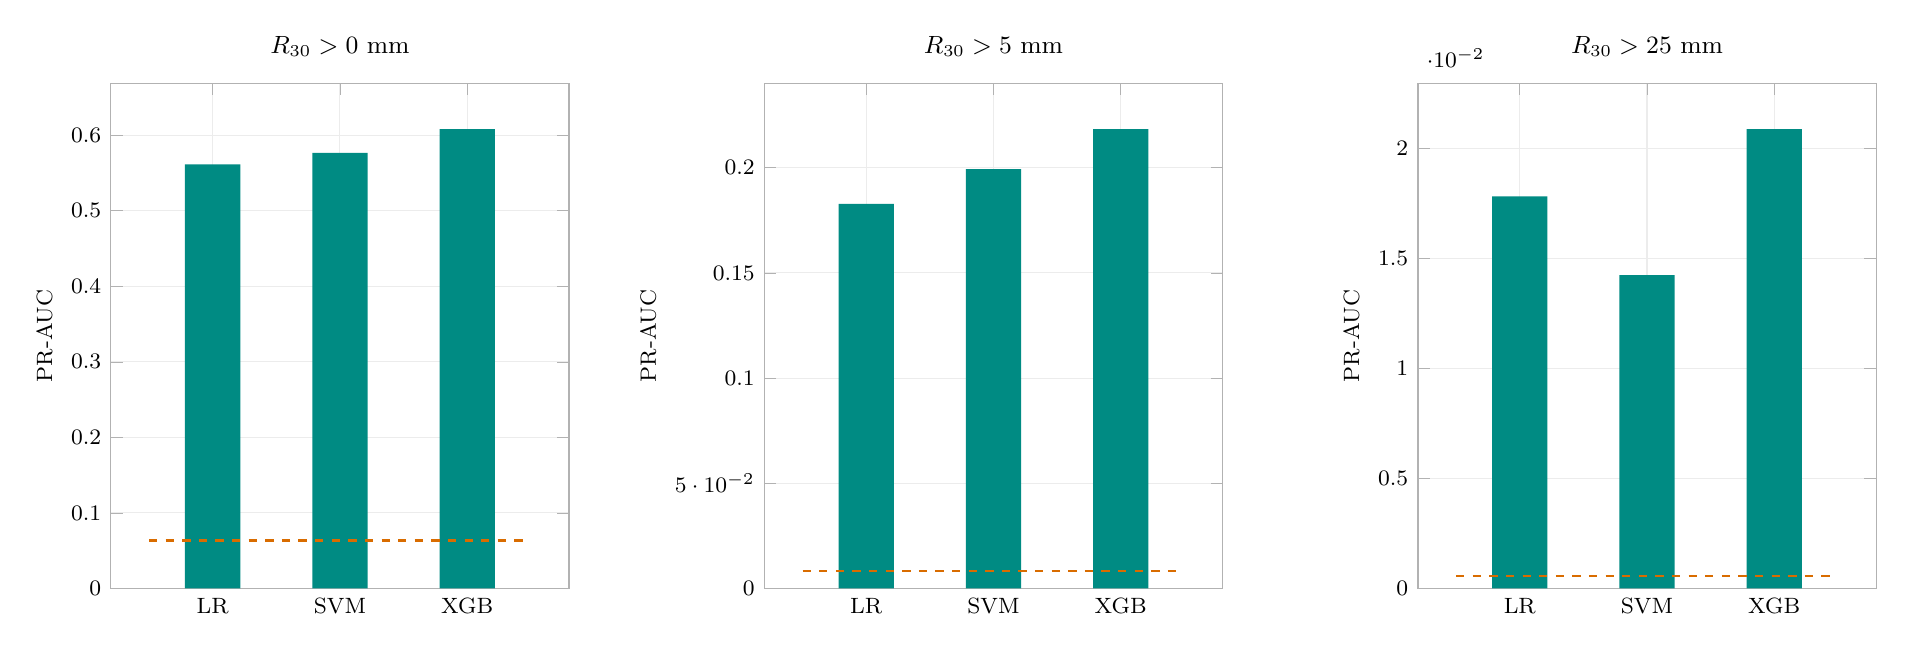
\begin{tikzpicture}
\begin{axis}[reportaxis,at={(0.0cm,0)},anchor=south west,width=7.4cm,height=8cm,title={$R_{30}>0$ mm},ylabel={PR-AUC},xtick={0,1,2},xticklabels={LR,SVM,XGB},ymin=0]
\addplot[ybar,bar width=20pt,fill=teal,draw=none] coordinates {(0,0.561335708) (1,0.576651539) (2,0.608087093)};
\addplot[orange!85!black,dashed,thick] coordinates {(-0.5,0.0636020906) (2.5,0.0636020906)};
\end{axis}
\begin{axis}[reportaxis,at={(8.3cm,0)},anchor=south west,width=7.4cm,height=8cm,title={$R_{30}>5$ mm},ylabel={PR-AUC},xtick={0,1,2},xticklabels={LR,SVM,XGB},ymin=0]
\addplot[ybar,bar width=20pt,fill=teal,draw=none] coordinates {(0,0.182820914) (1,0.199347496) (2,0.218385089)};
\addplot[orange!85!black,dashed,thick] coordinates {(-0.5,0.0083446859) (2.5,0.0083446859)};
\end{axis}
\begin{axis}[reportaxis,at={(16.6cm,0)},anchor=south west,width=7.4cm,height=8cm,title={$R_{30}>25$ mm},ylabel={PR-AUC},xtick={0,1,2},xticklabels={LR,SVM,XGB},ymin=0]
\addplot[ybar,bar width=20pt,fill=teal,draw=none] coordinates {(0,0.0178296999) (1,0.0142504086) (2,0.0208893976)};
\addplot[orange!85!black,dashed,thick] coordinates {(-0.5,0.000551731625) (2.5,0.000551731625)};
\end{axis}
\end{tikzpicture}\end{center}

\textbf{测试比较。}图 8 为原算法比较，三个 XGBoost 的测试 PR-AUC 为 0.60809、0.21839、0.02089。最终网格模型分别为 0.61218、0.22511、0.02118，均略高；但 25 mm 的 ROC-AUC 与 F1 下降，因此不能称为所有性能均改善。最终 5 mm 的 PR-AUC 也低于此前单独调参模型的 0.22640。测试结果用于报告，不用于重新选择参数或模型。

\clearpage\section*{图 9：最终选定模型的 ROC 与 PR 曲线}
\begin{center}\begin{tikzpicture}
\begin{axis}[reportaxis,at={(0.0cm,6.4cm)},anchor=south west,width=7.4cm,height=5.4cm,title={$R_{30}>0$ mm: ROC (XGB)},xlabel={假正例率（FPR）},ylabel={真正例率（TPR）},xmin=0,xmax=1,xtick={0,0.2,0.4,0.6,0.8,1},ymin=0,ymax=1,ytick={0,0.2,0.4,0.6,0.8,1},scaled ticks=false,legend style={at={(0.97,0.05)},anchor=south east,draw=none,fill=white,font=\scriptsize}]
\addplot[teal,thick,no marks] coordinates {(0,0) (0.0002440926071,0.1130676072) (0.0009765379593,0.1972251683) (0.002685521271,0.2901931283) (0.004150244444,0.3399033125) (0.006347580501,0.3925560516) (0.009277194379,0.4422045729) (0.01293942114,0.4858199936) (0.01806653861,0.5313839627) (0.02294906087,0.5629257825) (0.0266111201,0.5824926621) (0.0292968089,0.5950127026) (0.03344722088,0.6127790247) (0.03686535503,0.6248575586) (0.04004324979,0.6394322078) (0.04199213744,0.6468120267) (0.04492158378,0.6556125595) (0.04931608837,0.6668648102) (0.05200177717,0.6729398416) (0.05639577916,0.6807858323) (0.06176816195,0.6880891893) (0.07104770176,0.6974397553) (0.07593340711,0.7032854007) (0.07910158508,0.7060010359) (0.08451601814,0.7116863577) (0.1017519382,0.7316182818) (0.1076703044,0.7373948647) (0.1137706092,0.7425326197) (0.1208554935,0.7492834768) (0.1313476224,0.7579458846) (0.1415839315,0.7650050564) (0.1743168004,0.7851565005) (0.1860367637,0.791823496) (0.1984896749,0.798473226) (0.2075175832,0.8027304344) (0.2377921028,0.8188392571) (0.2934356679,0.8450065363) (0.3090820543,0.8516562662) (0.3161647607,0.8550156624) (0.3293522952,0.8600152924) (0.3373993097,0.8635670769) (0.3439862919,0.8660459265) (0.3537566975,0.8704387934) (0.3911139234,0.8849049158) (0.4001547316,0.8879337987) (0.4121105785,0.8914411859) (0.4201525671,0.8942702809) (0.4350593043,0.8987420763) (0.4567842164,0.9048615051) (0.4824276777,0.9114939694) (0.5078020843,0.9172434206) (0.5683591649,0.9293515527) (0.5854481604,0.9324075673) (0.5959438074,0.9348987495) (0.6188972241,0.9396443282) (0.6310916351,0.9425844165) (0.6367174922,0.9436030881) (0.6508698375,0.9471746047) (0.6953219995,0.9574155835) (0.7594178366,0.969797499) (0.7967192747,0.975307698) (0.8339754795,0.9796611006) (0.8830695893,0.9868066004) (0.9299355374,0.9922354044) (0.9563114441,0.9961818316) (0.9841063379,0.9988999334) (1,1)};
\addlegendentry{AUC = 0.88002}
\addplot[orange!85!black,dashed,thick,no marks] coordinates {(0,0) (1,1)};
\addlegendentry{随机参考}
\end{axis}
\begin{axis}[reportaxis,at={(8.3cm,6.4cm)},anchor=south west,width=7.4cm,height=5.4cm,title={$R_{30}>5$ mm: ROC (XGB)},xlabel={假正例率（FPR）},ylabel={真正例率（TPR）},xmin=0,xmax=1,xtick={0,0.2,0.4,0.6,0.8,1},ymin=0,ymax=1,ytick={0,0.2,0.4,0.6,0.8,1},scaled ticks=false,legend style={at={(0.97,0.05)},anchor=south east,draw=none,fill=white,font=\scriptsize}]
\addplot[teal,thick,no marks] coordinates {(0,0) (0.0007322880498,0.09785122103) (0.002197180541,0.1909461771) (0.004150265065,0.2714454909) (0.00756824208,0.3576974414) (0.01074212308,0.410035155) (0.01391600408,0.4486304589) (0.01684563086,0.4727689734) (0.02075195811,0.4985618408) (0.02563466942,0.5393942812) (0.02734349973,0.5497151881) (0.02929705884,0.5598856992) (0.03320306969,0.5770308123) (0.03662041393,0.5877841069) (0.04175038517,0.6015077172) (0.04314614612,0.6049480195) (0.04638678572,0.610738255) (0.05246355843,0.6247438573) (0.0581113043,0.634575978) (0.06225555793,0.6439381122) (0.06444467049,0.6477920027) (0.06546455838,0.6489011712) (0.06836745009,0.6540898238) (0.07055782821,0.6573045326) (0.0719673522,0.6605944391) (0.07568336997,0.665632696) (0.07666022863,0.6665350704) (0.07885740917,0.6705393567) (0.08398453289,0.6779087474) (0.08571250488,0.6810294588) (0.08862378096,0.6841689696) (0.09033102932,0.6867820954) (0.09254972448,0.6893576222) (0.09691924883,0.6960314327) (0.1025530735,0.7019908635) (0.1049389815,0.7051679732) (0.1101121402,0.7102438291) (0.1115721286,0.7124621661) (0.1162066308,0.7172372305) (0.1176905068,0.7183651984) (0.1186521787,0.71971876) (0.1225586641,0.7234034553) (0.1232771891,0.7244562254) (0.1254905056,0.7260541801) (0.1298823356,0.73133683) (0.1330566912,0.7340815521) (0.1369541595,0.7389506138) (0.1474406382,0.7484819431) (0.1481972884,0.7487639351) (0.1511375143,0.7511514673) (0.1518552484,0.7520914406) (0.15477744,0.7544977723) (0.1577156093,0.7562273231) (0.1608956599,0.7593480345) (0.1643084165,0.7611527833) (0.1687021448,0.7640667005) (0.1713867264,0.7661158423) (0.1731248229,0.7680709868) (0.1745470026,0.7686913692) (0.1769933414,0.7707217115) (0.1787178331,0.7714548907) (0.1818885502,0.7738424229) (0.1838095209,0.7758727652) (0.1892111143,0.7787490835) (0.1908974808,0.7805538323) (0.1923959108,0.7814562066) (0.1957947461,0.7847085143) (0.1984750564,0.7861372737) (0.2006913786,0.7879608219) (0.2089874793,0.7919087098) (0.2106422067,0.793450266) (0.2124211177,0.7941458463) (0.2183145415,0.7983569267) (0.2198890637,0.799014908) (0.2203926007,0.7996540898) (0.2221952411,0.800105277) (0.2250975,0.8021920177) (0.2284585265,0.8036019777) (0.2297233014,0.8048051435) (0.234371883,0.8076814618) (0.2438970064,0.8126633204) (0.2451220741,0.8141296787) (0.2473190965,0.8152576467) (0.2485300848,0.8165360104) (0.2529032476,0.8183595586) (0.2551314346,0.8201455079) (0.2600100328,0.8224390427) (0.2609740776,0.8233602166) (0.2622076879,0.8236798075) (0.2635007798,0.8248453744) (0.2673348116,0.8261049386) (0.2727035002,0.8293760457) (0.2773440139,0.8310867971) (0.2822262506,0.8340759122) (0.2849233296,0.834790292) (0.2922500068,0.8381553964) (0.2927182662,0.8387193804) (0.298095972,0.841689696) (0.3012782373,0.8439456319) (0.3064047283,0.8465211588) (0.3071276828,0.8474235332) (0.3107720379,0.8497734664) (0.3108704356,0.8501870547) (0.3149313201,0.852781381) (0.315430744,0.8537589532) (0.320558026,0.8563156806) (0.321268483,0.856936063) (0.3249558673,0.858308424) (0.3291224266,0.8607523546) (0.3323008952,0.8620871167) (0.3376501258,0.8653582238) (0.3420213903,0.8672005715) (0.3449692096,0.8690053202) (0.3473668241,0.869400109) (0.3525762096,0.8717500423) (0.3544981296,0.872220029) (0.3557095925,0.8731600023) (0.357345811,0.8737803846) (0.3587243286,0.874964751) (0.3623106259,0.8766379035) (0.364501004,0.8782170586) (0.3706102068,0.8803601978) (0.3732811836,0.8821649465) (0.3767246301,0.883274115) (0.3776821889,0.8841576899) (0.3806206746,0.8852292595) (0.3825661658,0.8866392194) (0.3852651432,0.8873911981) (0.3915945545,0.8903991127) (0.3950270855,0.8914518828) (0.3957478252,0.8920534657) (0.3989262939,0.8934822251) (0.4008808022,0.8939710112) (0.4062290836,0.8961141504) (0.4067285075,0.8969601263) (0.4099525365,0.8982572895) (0.4147949079,0.9012088057) (0.4206541615,0.9033519448) (0.4216297546,0.9041415224) (0.4243250935,0.9050062978) (0.4284152442,0.9072246348) (0.4367694027,0.9098377606) (0.4392090973,0.910984528) (0.4404145488,0.9119433008) (0.4456168154,0.913202865) (0.4477530906,0.9146316245) (0.4497077571,0.9150076138) (0.4538553328,0.9171319535) (0.4606954,0.9196322824) (0.4643623771,0.9217002237) (0.4667791333,0.9224334029) (0.4704608226,0.924614141) (0.4729009918,0.9252533228) (0.4767979855,0.9273212641) (0.4885275663,0.930949561) (0.4890174985,0.9314759461) (0.4946440462,0.9329047055) (0.4999888472,0.9353486361) (0.5019571185,0.9357246254) (0.5039057736,0.9366833982) (0.506351005,0.9372473822) (0.5097643943,0.9389017352) (0.5188237894,0.9417028556) (0.5231929974,0.9434324065) (0.5249043588,0.9437143985) (0.5253677141,0.9441843852) (0.5297604932,0.945951535) (0.5366329905,0.9476998853) (0.5395477469,0.9490158479) (0.5434600856,0.9500686181) (0.5481202155,0.9518921663) (0.5551831804,0.9536781155) (0.5610310439,0.9558024552) (0.5622860106,0.9558964525) (0.5651841564,0.9569868216) (0.5688642638,0.9575884045) (0.5720158392,0.958697573) (0.5776343189,0.9600887335) (0.5890652262,0.9620626774) (0.5913084417,0.9628710545) (0.5944894415,0.9632846427) (0.5954550682,0.9638862256) (0.5991210961,0.964224616) (0.6020429713,0.9650141936) (0.6115744225,0.9660481642) (0.6152314332,0.9668565413) (0.6357489453,0.9688680841) (0.6413519218,0.9699584532) (0.6638676041,0.9718383998) (0.6745576808,0.9736055496) (0.6885032675,0.9749403117) (0.6899306676,0.9754290978) (0.7070317845,0.9769894535) (0.7094717955,0.9775910364) (0.7355880127,0.9797341755) (0.7563488298,0.9807305473) (0.7629245519,0.9814261275) (0.7851686121,0.9828924859) (0.8015119715,0.9849980261) (0.8266654095,0.9871411652) (0.8288567368,0.9877427481) (0.8427675205,0.9890775102) (0.8540076437,0.9899046867) (0.8557006544,0.9904310718) (0.8623061173,0.9910702536) (0.8632720604,0.9914838419) (0.86938506,0.9917846333) (0.8740176638,0.9927622056) (0.882323889,0.9935329837) (0.895996588,0.9942661628) (0.929924827,0.9976500667) (0.93799012,0.9980072566) (0.9414038258,0.9984584438) (0.9521516439,0.9985524411) (0.9890068203,0.9999248021) (1,1)};
\addlegendentry{AUC = 0.88159}
\addplot[orange!85!black,dashed,thick,no marks] coordinates {(0,0) (1,1)};
\addlegendentry{随机参考}
\end{axis}
\begin{axis}[reportaxis,at={(16.6cm,6.4cm)},anchor=south west,width=7.4cm,height=5.4cm,title={$R_{30}>25$ mm: ROC (XGB)},xlabel={假正例率（FPR）},ylabel={真正例率（TPR）},xmin=0,xmax=1,xtick={0,0.2,0.4,0.6,0.8,1},ymin=0,ymax=1,ytick={0,0.2,0.4,0.6,0.8,1},scaled ticks=false,legend style={at={(0.97,0.05)},anchor=south east,draw=none,fill=white,font=\scriptsize}]
\addplot[teal,thick,no marks] coordinates {(0,0) (0.0007323858151,0.07648564117) (0.00292954326,0.2015922661) (0.004394471853,0.265851578) (0.007324172075,0.3525732158) (0.009277410198,0.384987205) (0.0102538723,0.4077338641) (0.01367172509,0.4557861814) (0.01562496321,0.4754051749) (0.01855497736,0.4964458345) (0.01928704925,0.5109468297) (0.02050146611,0.5211828263) (0.02075182088,0.5277224908) (0.02197251623,0.5373898209) (0.02246098272,0.5373898209) (0.02258466896,0.5379584873) (0.02293924667,0.5419391527) (0.02319336853,0.5419391527) (0.02416857494,0.5490474837) (0.02442410946,0.5493318169) (0.02612291179,0.5678134774) (0.02661137829,0.5695194768) (0.02679706462,0.5729314757) (0.02783191667,0.5803241399) (0.02832038316,0.5820301393) (0.02856995313,0.5851578049) (0.02905276898,0.5860108047) (0.0295191038,0.5897071368) (0.03027346432,0.5916974694) (0.03100114127,0.597099801) (0.03149415967,0.5979528007) (0.03173823595,0.6005117998) (0.03320316455,0.6059141314) (0.03341757497,0.6081887973) (0.03370277536,0.6081887973) (0.03393523644,0.6093261302) (0.03442401686,0.6093261302) (0.03491373905,0.6098947967) (0.03515216469,0.6116007961) (0.03541821569,0.6116007961) (0.03637662713,0.6144441285) (0.03687215692,0.6147284618) (0.03832531335,0.6204151265) (0.03833457412,0.6218367927) (0.03905942575,0.622121126) (0.04003902709,0.6278077907) (0.04077204076,0.628092124) (0.04125972244,0.6306511231) (0.04199226521,0.6315041228) (0.04344353809,0.64003412) (0.04399086543,0.6403184532) (0.0446810284,0.6414557862) (0.04564948542,0.6445834518) (0.04589827057,0.644867785) (0.0466339526,0.644867785) (0.04711927984,0.6457207848) (0.04760727545,0.6482797839) (0.04785166566,0.6482797839) (0.048074709,0.6491327836) (0.04835410179,0.6491327836) (0.04906592555,0.6514074495) (0.05054294024,0.6533977822) (0.05102512824,0.6548194484) (0.05151406562,0.6551037816) (0.05195544344,0.6582314473) (0.05254232526,0.6585157805) (0.0534666759,0.6627807791) (0.05373712184,0.6627807791) (0.05395498543,0.6633494456) (0.05444345192,0.6633494456) (0.05591199064,0.6653397782) (0.05638209255,0.6678987774) (0.05688484261,0.6678987774) (0.058105381,0.6715951095) (0.05859416141,0.6715951095) (0.05937222324,0.6752914416) (0.06153469203,0.6772817742) (0.06176731007,0.678134774) (0.06249985285,0.6787034404) (0.06302944345,0.6787034404) (0.06396478144,0.6801251066) (0.06468994699,0.6801251066) (0.06542955307,0.682968439) (0.06567441417,0.682968439) (0.06713840098,0.6863804379) (0.06844840785,0.6869491044) (0.06927638367,0.6892237703) (0.07130072568,0.6926357691) (0.07202102541,0.6951947683) (0.07422367653,0.6977537674) (0.0751824019,0.7000284333) (0.07544405795,0.7000284333) (0.0759140029,0.702018766) (0.07740969609,0.7023030992) (0.07767935722,0.7045777651) (0.07883899426,0.707989764) (0.07887258417,0.709127097) (0.080141153,0.7094114302) (0.08129482547,0.7131077623) (0.08252760691,0.7133920955) (0.0839879836,0.715098095) (0.08471660232,0.7165197612) (0.08544930206,0.7168040944) (0.0860851561,0.7187944271) (0.08691407369,0.7190787603) (0.08715814997,0.71993176) (0.08740238322,0.71993176) (0.08764614558,0.7219220927) (0.08886762574,0.7230594256) (0.08959765712,0.7264714245) (0.09064255476,0.7273244242) (0.09123712772,0.7290304237) (0.09155277879,0.7290304237) (0.09179685507,0.7304520898) (0.0925345776,0.7313050896) (0.09301739346,0.7332954222) (0.09472671226,0.7335797555) (0.09570097689,0.7347170884) (0.0971687308,0.7347170884) (0.09815633722,0.7364230879) (0.09839052488,0.7381290873) (0.09908476887,0.7381290873) (0.09985105853,0.7404037532) (0.1005911355,0.7406880864) (0.1013258757,0.7415410862) (0.1018064941,0.7443844185) (0.1027831132,0.7455217515) (0.1036115599,0.7455217515) (0.1037589474,0.746090418) (0.1048071413,0.7463747512) (0.1052106912,0.7469434177) (0.1062012799,0.7469434177) (0.1069255037,0.7483650839) (0.107177742,0.7483650839) (0.1083695563,0.7517770827) (0.1088870608,0.7517770827) (0.1096244694,0.7523457492) (0.1105926125,0.7551890816) (0.1113281376,0.7554734148) (0.112061936,0.7563264146) (0.1127944788,0.7563264146) (0.1137695283,0.758032414) (0.1149938337,0.7583167472) (0.1154807306,0.7588854137) (0.1157017334,0.7603070799) (0.116210919,0.7608757464) (0.1181674533,0.7608757464) (0.1184080764,0.7614444129) (0.1196411718,0.7617287461) (0.1201170813,0.7631504123) (0.1206055478,0.7631504123) (0.1208066164,0.7637190788) (0.1216369467,0.7637190788) (0.1218190229,0.7645720785) (0.1230469385,0.7648564117) (0.1234526859,0.7662780779) (0.1249096094,0.7662780779) (0.1257344459,0.7668467444) (0.1262136517,0.7676997441) (0.1269735059,0.7676997441) (0.1271935669,0.7688370771) (0.1279505958,0.7688370771) (0.1286621057,0.7694057435) (0.1296407652,0.7694057435) (0.1301129076,0.7702587432) (0.1310958052,0.7705430765) (0.1315740691,0.7713960762) (0.1333320462,0.7713960762) (0.1349639827,0.7739550753) (0.136230511,0.7742394086) (0.1367153673,0.7753767415) (0.1394207685,0.7756610748) (0.1398362476,0.7762297413) (0.1405297068,0.7762297413) (0.1405954739,0.7765140745) (0.1411183152,0.7765140745) (0.1418361035,0.777082741) (0.1428254365,0.777082741) (0.1430618216,0.7785044072) (0.1438131999,0.7793574069) (0.1445201578,0.781916406) (0.1452669841,0.7822007393) (0.1457311215,0.7833380722) (0.146256945,0.7833380722) (0.146472925,0.7841910719) (0.1472243033,0.7844754052) (0.1477030381,0.7861814046) (0.1479493119,0.7861814046) (0.1484784316,0.7873187376) (0.1491698503,0.7901620699) (0.1496474864,0.7901620699) (0.1501130364,0.7910150697) (0.1516512663,0.7915837361) (0.1518454286,0.7924367359) (0.1523437837,0.7924367359) (0.152575617,0.7935740688) (0.1541523027,0.7941427353) (0.1545384298,0.7958487347) (0.1555373375,0.7958487347) (0.1564902552,0.7972704009) (0.1569592584,0.7972704009) (0.1569947319,0.7981234006) (0.1579639737,0.7984077339) (0.1582526273,0.7992607336) (0.1589005674,0.7992607336) (0.1595160163,0.8012510662) (0.159912189,0.8012510662) (0.1601561084,0.8026727324) (0.1606464584,0.8026727324) (0.1613744493,0.8038100654) (0.1628418893,0.8040943986) (0.1629359096,0.8046630651) (0.1633480925,0.8046630651) (0.1635604624,0.8058003981) (0.1667398896,0.8060847313) (0.166754644,0.8066533978) (0.1672222345,0.8072220643) (0.1677697188,0.8072220643) (0.167989152,0.808075064) (0.1689485052,0.808075064) (0.1694332046,0.8086437305) (0.1701538183,0.8086437305) (0.1704026034,0.8092123969) (0.170907237,0.8092123969) (0.1711246297,0.8097810634) (0.1741648314,0.8103497299) (0.1745589636,0.8112027296) (0.1750681491,0.8112027296) (0.1755068585,0.8120557293) (0.1762645153,0.8126243958) (0.1763141153,0.8131930623) (0.1782263863,0.8131930623) (0.1791802459,0.8137617287) (0.1803946627,0.8137617287) (0.1804213463,0.814046062) (0.1823816477,0.814046062) (0.1835937101,0.8146147285) (0.1845853976,0.8146147285) (0.1848100105,0.8157520614) (0.186528904,0.8160363947) (0.1869432844,0.8171737276) (0.1875000294,0.8171737276) (0.1882197013,0.8197327268) (0.189210133,0.8197327268) (0.1901814154,0.8217230594) (0.1906814971,0.8217230594) (0.1918899494,0.8225760591) (0.1933606856,0.8225760591) (0.1935987973,0.8231447256) (0.1941993348,0.8231447256) (0.1943289856,0.8237133921) (0.1962994896,0.8237133921) (0.1975476533,0.824850725) (0.1981412845,0.825988058) (0.1994855092,0.825988058) (0.1999628313,0.8262723912) (0.2001952924,0.8274097242) (0.201173795,0.8274097242) (0.2014071979,0.8279783907) (0.202882329,0.8282627239) (0.2036103199,0.8296843901) (0.2045746959,0.8305373898) (0.2058029254,0.8339493887) (0.2067884913,0.8339493887) (0.2070291145,0.8348023884) (0.2079671208,0.8348023884) (0.2081061894,0.8353710549) (0.2093083632,0.8353710549) (0.2094800798,0.8362240546) (0.2102493518,0.8362240546) (0.2106665574,0.8367927211) (0.2111826493,0.8367927211) (0.2114154243,0.8376457208) (0.2124364636,0.8382143873) (0.2126422411,0.8393517202) (0.2153914348,0.8393517202) (0.2163002462,0.8399203867) (0.2171308903,0.8399203867) (0.2177731798,0.8407733864) (0.2194854809,0.8407733864) (0.2197162154,0.8413420529) (0.220952607,0.8419107194) (0.2219088209,0.8441853853) (0.2236730765,0.8441853853) (0.2238575072,0.8447540517) (0.2246098272,0.8447540517) (0.2250953114,0.8456070515) (0.2260785229,0.8456070515) (0.2269961241,0.8464600512) (0.2284053311,0.8470287177) (0.2287556708,0.8487347171) (0.2299871966,0.8487347171) (0.2304207263,0.8493033836) (0.230501091,0.8507250498) (0.2317005964,0.8507250498) (0.2321728958,0.8518623827) (0.2329194082,0.8518623827) (0.233581318,0.8524310492) (0.2370607,0.8527153824) (0.2372947307,0.8541370486) (0.2387445909,0.8564117145) (0.2418001748,0.856980381) (0.2426612697,0.8586863804) (0.243408253,0.8586863804) (0.243657666,0.8589707137) (0.2438934233,0.8603923799) (0.2460962314,0.8606767131) (0.2465109256,0.8612453796) (0.2483170901,0.8612453796) (0.2492687522,0.8623827125) (0.2495076487,0.8635200455) (0.2514699906,0.8635200455) (0.2519703862,0.8638043787) (0.253409887,0.8672163776) (0.2558605384,0.8675007108) (0.2563242049,0.8683537105) (0.2575701711,0.8686380438) (0.2582997316,0.8694910435) (0.2593837129,0.8694910435) (0.2602338204,0.87005971) (0.2646576442,0.87005971) (0.2648896344,0.8711970429) (0.2653319539,0.8714813762) (0.2690508603,0.8717657094) (0.2709948377,0.8729030424) (0.2736840717,0.8731873756) (0.2739046037,0.8740403753) (0.2749047671,0.8740403753) (0.2751165091,0.8746090418) (0.2773624818,0.8746090418) (0.2775100264,0.8751777083) (0.2792358262,0.8754620415) (0.2793088136,0.8763150412) (0.279785194,0.8763150412) (0.280516795,0.8777367074) (0.2825017395,0.8777367074) (0.282953006,0.8783053739) (0.2839355896,0.8783053739) (0.2844152662,0.8788740404) (0.2871462522,0.8791583736) (0.2873501462,0.880864373) (0.28857712,0.880864373) (0.2892903564,0.8817173728) (0.2910062677,0.8817173728) (0.291046607,0.8822860392) (0.2944531585,0.8822860392) (0.2946799689,0.883139039) (0.295170162,0.883139039) (0.2954100003,0.8837077054) (0.2968890555,0.8837077054) (0.2971164938,0.8842763719) (0.2985842477,0.8842763719) (0.2986655541,0.8848450384) (0.3000888877,0.8848450384) (0.3002926247,0.8856980381) (0.3015221099,0.8856980381) (0.3029707145,0.8862667046) (0.3044447469,0.8862667046) (0.3046735978,0.8871197043) (0.3078629136,0.8871197043) (0.3083377244,0.8888257037) (0.3137483698,0.8893943702) (0.3139583852,0.8899630367) (0.3147416268,0.8899630367) (0.3149282549,0.8902473699) (0.3151583616,0.8911003696) (0.3156397648,0.8913847029) (0.3157282915,0.8925220358) (0.3169197918,0.8925220358) (0.3173927191,0.8928063691) (0.3178524615,0.893943702) (0.3192765799,0.893943702) (0.3207330325,0.895081035) (0.322023576,0.895081035) (0.3222284118,0.8965027012) (0.3240306522,0.8965027012) (0.3241910676,0.8967870344) (0.3256862899,0.8967870344) (0.3273734771,0.8973557009) (0.3290882895,0.8973557009) (0.3291939251,0.8987773671) (0.330570484,0.8993460336) (0.3308081248,0.9004833665) (0.3322835699,0.9004833665) (0.3325152461,0.901052033) (0.334228646,0.901052033) (0.3344719374,0.9021893659) (0.3347034567,0.9024736992) (0.3354738274,0.9024736992) (0.3356172909,0.9033266989) (0.33617796,0.9038953654) (0.3410756528,0.9041796986) (0.3412721695,0.9050326983) (0.3420656137,0.9050326983) (0.3430174327,0.905885698) (0.3452229091,0.905885698) (0.3454379474,0.9061700313) (0.3485621238,0.9064543645) (0.3486395062,0.907023031) (0.3503499238,0.907023031) (0.3507374635,0.9075916975) (0.3513191656,0.9075916975) (0.3515488014,0.9087290304) (0.3557017083,0.9087290304) (0.3559471973,0.9092976969) (0.3574684753,0.9095820301) (0.3576602832,0.9101506966) (0.3596215264,0.9101506966) (0.3601088941,0.9121410293) (0.3646094725,0.9121410293) (0.3647512094,0.914131362) (0.3752511984,0.914131362) (0.3754665506,0.9147000284) (0.3764802128,0.9152686949) (0.3766797118,0.9158373614) (0.3776938448,0.9158373614) (0.3779283464,0.9169746943) (0.3796461412,0.9169746943) (0.379875463,0.9178276941) (0.3806381425,0.9183963605) (0.3828315329,0.9183963605) (0.3830542623,0.9186806938) (0.3855056986,0.9186806938) (0.3857193242,0.918965027) (0.3894255166,0.9192493603) (0.3901368695,0.9195336935) (0.3903785914,0.92010236) (0.3908761617,0.92010236) (0.3911106632,0.9209553597) (0.3916071348,0.9209553597) (0.3925770045,0.9220926926) (0.3942872651,0.9220926926) (0.3945217667,0.9229456924) (0.3969829346,0.9232300256) (0.3972166514,0.9240830253) (0.3994141227,0.9240830253) (0.4003686101,0.9246516918) (0.4011366264,0.9246516918) (0.4013384798,0.9257890247) (0.4038255465,0.9257890247) (0.4040413696,0.9263576912) (0.4101611704,0.9263576912) (0.4103994391,0.9269263577) (0.4163873916,0.9272106909) (0.4165051133,0.9277793574) (0.4177352264,0.9277793574) (0.4179626646,0.9280636906) (0.4250766643,0.9280636906) (0.4252924874,0.9283480239) (0.4274788144,0.9283480239) (0.4277343489,0.9311913563) (0.4328632471,0.9314756895) (0.4330856626,0.9317600227) (0.4401357786,0.932044356) (0.4402141028,0.9328973557) (0.4409028531,0.9337503554) (0.441663963,0.9337503554) (0.4418877911,0.9340346887) (0.4460457209,0.9340346887) (0.4465330887,0.9357406881) (0.4470237526,0.9357406881) (0.4472648466,0.9363093546) (0.4484878964,0.9363093546) (0.4487046613,0.9374466875) (0.4521485698,0.9377310208) (0.4523811878,0.938015354) (0.4550578649,0.938015354) (0.4551068371,0.9388683537) (0.4557899368,0.9388683537) (0.4558855268,0.9400056867) (0.4572686781,0.9400056867) (0.4573327187,0.9408586864) (0.4594104278,0.9408586864) (0.4594879672,0.9411430196) (0.4606328498,0.9411430196) (0.460711017,0.9414273529) (0.4626644121,0.9414273529) (0.4628883972,0.9419960193) (0.4643734169,0.9419960193) (0.4648275087,0.9431333523) (0.4695057683,0.9431333523) (0.4704536633,0.9442706852) (0.4704768937,0.9448393517) (0.4758363694,0.9448393517) (0.4760741672,0.945123685) (0.4780583269,0.945123685) (0.4782630056,0.9456923514) (0.4824278417,0.9459766847) (0.4826457053,0.9462610179) (0.4836540307,0.9462610179) (0.483885707,0.9476826841) (0.4880378292,0.9476826841) (0.4882230446,0.9479670173) (0.4890172735,0.9479670173) (0.4892497346,0.9491043503) (0.4929242207,0.9493886835) (0.4931571526,0.94995735) (0.4944624506,0.94995735) (0.4946153319,0.9502416833) (0.5058742334,0.9502416833) (0.5061005729,0.951094683) (0.5085557763,0.951094683) (0.5090067288,0.9525163492) (0.5097818084,0.9525163492) (0.5099882137,0.9528006824) (0.5207672817,0.9530850156) (0.5209718035,0.9542223486) (0.5256392326,0.9547910151) (0.5261005447,0.9553596815) (0.5261311523,0.9562126813) (0.5273455692,0.9562126813) (0.5275620201,0.9567813477) (0.5329681136,0.9567813477) (0.5344394776,0.9573500142) (0.5349056555,0.9582030139) (0.5361418901,0.9582030139) (0.5363219258,0.9593403469) (0.5400427157,0.9593403469) (0.5402601084,0.9604776798) (0.5417656902,0.9604776798) (0.5419903032,0.9610463463) (0.543711865,0.9613306796) (0.5439451109,0.961899346) (0.5456577259,0.961899346) (0.5458853212,0.9624680125) (0.5507856823,0.9627523457) (0.5510242649,0.9641740119) (0.5519539523,0.9641740119) (0.5520203473,0.9653113449) (0.5527342116,0.9655956781) (0.5546868219,0.9655956781) (0.5547059713,0.9661643446) (0.5578667199,0.9664486779) (0.5585623766,0.9687233438) (0.5687707298,0.969007677) (0.5689094844,0.9698606767) (0.5717903694,0.9698606767) (0.5720184355,0.9707136764) (0.5730013331,0.9707136764) (0.5732245334,0.9712823429) (0.5827775693,0.9712823429) (0.5828715897,0.9724196759) (0.5837356668,0.9724196759) (0.5839722089,0.9732726756) (0.5852470562,0.9732726756) (0.5854459274,0.9735570088) (0.5912529024,0.9735570088) (0.5913081531,0.9746943418) (0.5942422483,0.9746943418) (0.5944811448,0.974978675) (0.596720839,0.974978675) (0.5969233203,0.9752630082) (0.6136512572,0.9755473415) (0.6142566606,0.9764003412) (0.6152678113,0.9764003412) (0.6162094278,0.9769690077) (0.6179347568,0.9769690077) (0.6181529343,0.9781063406) (0.6186194261,0.9783906739) (0.6208661836,0.9783906739) (0.6210743155,0.9789593403) (0.6257384485,0.9789593403) (0.6259745197,0.9812340063) (0.6266970169,0.9815183395) (0.6267246422,0.982087006) (0.6299277707,0.9823713392) (0.6301076494,0.9829400057) (0.646491682,0.9832243389) (0.6467260266,0.9837930054) (0.6521049657,0.9837930054) (0.6523432344,0.9840773386) (0.6613954037,0.9840773386) (0.6616181332,0.9846460051) (0.6630912238,0.9846460051) (0.6633010823,0.9852146716) (0.664778097,0.9852146716) (0.6649392972,0.9860676713) (0.6660407013,0.9863520045) (0.6662584079,0.986920671) (0.6711509209,0.986920671) (0.6718263294,0.9883423372) (0.6748134778,0.9883423372) (0.6757781678,0.9889110037) (0.676517146,0.9889110037) (0.6769976074,0.9897640034) (0.67822568,0.9897640034) (0.6783388498,0.9900483367) (0.6848549802,0.9900483367) (0.6850521248,0.9909013364) (0.7065736885,0.9909013364) (0.7072778211,0.9911856696) (0.7075164037,0.9920386693) (0.7204612367,0.9920386693) (0.7206954243,0.9926073358) (0.737320237,0.9926073358) (0.7374797107,0.992891669) (0.7407759177,0.992891669) (0.7409633306,0.9931760023) (0.7597645818,0.9931760023) (0.7598055489,0.9937446688) (0.7720063808,0.9937446688) (0.7721160974,0.9948820017) (0.7822363949,0.9948820017) (0.7824693268,0.9957350014) (0.8130099409,0.9957350014) (0.8132072424,0.9963036679) (0.8334564702,0.9965880011) (0.8336168856,0.9971566676) (0.9163097738,0.9971566676) (0.9165007968,0.9974410009) (0.9235906243,0.9974410009) (0.9237155662,0.9980096673) (0.9472556643,0.9980096673) (0.947319391,0.998862667) (0.9528965733,0.998862667) (0.9531155357,0.9991470003) (0.9883176143,0.9991470003) (0.9885128754,1) (1,1)};
\addlegendentry{AUC = 0.90309}
\addplot[orange!85!black,dashed,thick,no marks] coordinates {(0,0) (1,1)};
\addlegendentry{随机参考}
\end{axis}
\begin{axis}[reportaxis,at={(0.0cm,0.0cm)},anchor=south west,width=7.4cm,height=5.4cm,title={$R_{30}>0$ mm: PR (XGB)},xlabel={Recall},ylabel={Precision},xmin=0,xmax=1,xtick={0,0.2,0.4,0.6,0.8,1},ymin=0,ymax=1,ytick={0,0.2,0.4,0.6,0.8,1},scaled ticks=false,legend style={at={(0.97,0.97)},anchor=north east,draw=none,fill=white,font=\scriptsize}]
\addplot[teal,thick,no marks] coordinates {(0,1) (0.0003305132822,0.9925925926) (0.001457711565,0.9983108108) (0.001460178083,0.9966329966) (0.002510914338,0.9980392157) (0.002528179957,0.9961127308) (0.003546851491,0.9972260749) (0.003731840268,0.9953947368) (0.004878770688,0.9929718876) (0.005386873196,0.9936305732) (0.005732185581,0.9931623932) (0.00584071233,0.9916247906) (0.007189897146,0.9925093633) (0.007828725057,0.9912554653) (0.01072441605,0.9922409859) (0.01326246208,0.9895104895) (0.01571171349,0.9895914246) (0.0181609649,0.9883221477) (0.02028463607,0.989055923) (0.02579976815,0.9874445388) (0.04365488494,0.9868413716) (0.06814986557,0.9822253822) (0.09379424315,0.9755765925) (0.1150013566,0.9686701431) (0.1660533261,0.9483047624) (0.1738080556,0.9435733319) (0.2046518511,0.9286281883) (0.2341291962,0.9109518051) (0.2483314012,0.9036899408) (0.2609871001,0.8958539704) (0.2710307575,0.8909031944) (0.3022642626,0.8730346444) (0.3447253533,0.8445752408) (0.3901388649,0.8098114908) (0.420203241,0.7843058721) (0.4379966949,0.7680499989) (0.4631354365,0.7430686918) (0.5261253484,0.6731263214) (0.5537232075,0.6379757195) (0.5693337937,0.6154118921) (0.5866684754,0.5921793968) (0.6015613053,0.5696364842) (0.613033076,0.5541121102) (0.6249907506,0.5348962885) (0.6394322078,0.5202954251) (0.6481982093,0.5095877714) (0.6713982685,0.4707173206) (0.6806674395,0.4507689418) (0.6882347138,0.4303643038) (0.6974890857,0.3998645356) (0.7033692623,0.3859371088) (0.7060552993,0.3771786966) (0.7162814789,0.3543553437) (0.7302222332,0.3306842463) (0.7441185901,0.3043802433) (0.7578102262,0.2818181568) (0.7768517377,0.2469017634) (0.7951656266,0.2189464648) (0.8073773524,0.202199058) (0.8339836717,0.1733159943) (0.8600596897,0.1506028754) (0.8859901833,0.1324307913) (0.931642947,0.09815384008) (0.9436030881,0.09145356825) (0.9697185704,0.07984643768) (0.9797375626,0.07385811522) (0.9965863404,0.06589375353) (1,0.06360209059)};
\addlegendentry{AUC = 0.61218}
\addplot[orange!85!black,dashed,thick,no marks] coordinates {(0,0.0636020906) (1,0.0636020906)};
\addlegendentry{随机参考}
\end{axis}
\begin{axis}[reportaxis,at={(8.3cm,0.0cm)},anchor=south west,width=7.4cm,height=5.4cm,title={$R_{30}>5$ mm: PR (XGB)},xlabel={Recall},ylabel={Precision},xmin=0,xmax=1,xtick={0,0.2,0.4,0.6,0.8,1},ymin=0,ymax=1,ytick={0,0.2,0.4,0.6,0.8,1},scaled ticks=false,legend style={at={(0.97,0.97)},anchor=north east,draw=none,fill=white,font=\scriptsize}]
\addplot[teal,thick,no marks] coordinates {(0,0) (0.0002255935931,0.75) (0.0002443930592,0.65) (0.0007519786438,0.8163265306) (0.0008647754404,0.8214285714) (0.000996371703,0.7910447761) (0.001428759423,0.8351648352) (0.001466358355,0.7878787879) (0.001748350347,0.8157894737) (0.001955144474,0.7878787879) (0.002387532194,0.8037974684) (0.004248679338,0.7197452229) (0.004775064388,0.7341040462) (0.005508243566,0.7043269231) (0.006636211532,0.7131313131) (0.00678660726,0.705078125) (0.007143797116,0.7116104869) (0.007726580565,0.7025641026) (0.008572556539,0.7113884555) (0.00953132931,0.7002762431) (0.01043370368,0.7070063694) (0.01137367699,0.6954022989) (0.01216325456,0.7002164502) (0.01240764762,0.6954689146) (0.01299043107,0.7001013171) (0.01323482413,0.6963402572) (0.01449438836,0.7034671533) (0.01483277875,0.6976127321) (0.01507717181,0.701048951) (0.01520876807,0.6992221262) (0.01643073337,0.7048387097) (0.01767149813,0.6973293769) (0.01806628692,0.701459854) (0.01812268532,0.6985507246) (0.01832947944,0.7004310345) (0.01928825221,0.6932432432) (0.02043501965,0.6999356085) (0.0207922095,0.6942875078) (0.02103660256,0.6954630205) (0.02156298761,0.6926328502) (0.02173218281,0.6942942943) (0.02182618014,0.6927207637) (0.02227736732,0.6942003515) (0.02291654917,0.6871476888) (0.02351813209,0.690397351) (0.02353693155,0.6886688669) (0.024119715,0.6901559978) (0.02725922584,0.6630086877) (0.02759761623,0.6639529625) (0.02851879007,0.650235748) (0.02876318313,0.652173913) (0.03015434362,0.6436597111) (0.03081232493,0.645784082) (0.03113191585,0.6396292005) (0.03139510838,0.6413210445) (0.0327674694,0.634048745) (0.03306826086,0.6357065414) (0.03513620213,0.6288694482) (0.03588818078,0.6306574166) (0.03695975034,0.6259153136) (0.03780572632,0.6274570983) (0.03829451244,0.6219847328) (0.03910288948,0.623501199) (0.03985486812,0.6191588785) (0.04100163555,0.6215445996) (0.04103923449,0.6182384594) (0.04128362754,0.6187658495) (0.04235519711,0.6154056269) (0.04256199124,0.616389872) (0.04415994586,0.6068199432) (0.04446073732,0.6076567318) (0.04457353411,0.6063938619) (0.0450811197,0.6070886076) (0.04639708232,0.6025390625) (0.04752505029,0.6039178213) (0.04854022146,0.5996284255) (0.04910420544,0.6001838235) (0.04942379636,0.5994072047) (0.04976218675,0.6003628941) (0.05075855846,0.5968169761) (0.05124734458,0.5980693287) (0.0514541387,0.5962962963) (0.05214971895,0.597329888) (0.05508243566,0.5889447236) (0.0558344143,0.5890519635) (0.05622920309,0.5878537736) (0.05666159081,0.5884420148) (0.05675558814,0.5874683791) (0.05731957212,0.5887236918) (0.05743236892,0.5875) (0.05809035023,0.5886835588) (0.05837234223,0.5876230129) (0.05955670859,0.5887381528) (0.06220743331,0.5807300807) (0.06279021676,0.5813751088) (0.06299701088,0.5802597403) (0.06391818472,0.5809979494) (0.0646513639,0.5791512294) (0.0648205591,0.5796906523) (0.06647491211,0.5738396624) (0.0669824977,0.5747701242) (0.06805406726,0.572875455) (0.06839245765,0.5734552333) (0.07173876262,0.5639964529) (0.0724719418,0.5630203009) (0.07294192845,0.563625799) (0.07316752204,0.5628344179) (0.0734119151,0.5634920635) (0.07373150603,0.562697274) (0.07391950069,0.5632430884) (0.07470907826,0.5627301048) (0.07474667719,0.5615819209) (0.07886376027,0.5555555556) (0.07910815333,0.5539028564) (0.07991653037,0.5540205917) (0.07999172823,0.5533879568) (0.08025492076,0.5539839086) (0.08044291542,0.5514885939) (0.08153328445,0.5511500826) (0.08296204388,0.5471791692) (0.08356362679,0.5477510783) (0.08440960277,0.5472940029) (0.08694753069,0.5427129782) (0.08756791307,0.5436507937) (0.09018103886,0.5382026254) (0.09108341323,0.5380344253) (0.09290696144,0.5353699491) (0.09341454703,0.5358567885) (0.09563288403,0.5318904224) (0.09670445359,0.5316246383) (0.09807681462,0.528357302) (0.09911078525,0.5282035868) (0.1005771436,0.5259535981) (0.1008591356,0.5244379277) (0.1019683041,0.5246662797) (0.1021562988,0.5232546943) (0.1034534619,0.5217597421) (0.1038670502,0.5221130221) (0.108660914,0.5131847643) (0.1111424436,0.5126159716) (0.1117628259,0.5114418445) (0.1132855827,0.51171875) (0.1135487752,0.509747658) (0.1143759517,0.5095477387) (0.11725227,0.5035117462) (0.1192074145,0.5017804859) (0.1215009494,0.4973451327) (0.1235500912,0.4969751966) (0.1273663828,0.4900188051) (0.1284755513,0.4900329844) (0.1291335326,0.4877858259) (0.1306374899,0.4861820472) (0.1320662493,0.4805390246) (0.1349049687,0.4764940239) (0.1354877521,0.476748032) (0.1367849153,0.4738521654) (0.1389844528,0.473152) (0.1434211268,0.4683241252) (0.1443986991,0.4683822184) (0.1470870227,0.4641395266) (0.1501513357,0.462478286) (0.1586674938,0.4510233527) (0.1651157107,0.446881042) (0.1671084541,0.443740016) (0.172992687,0.4385245902) (0.1747974358,0.4359118612) (0.1775045589,0.43403512) (0.1787265242,0.4343277445) (0.1807004681,0.4321359529) (0.1817908371,0.4322753688) (0.1841595699,0.4282778822) (0.1880510593,0.4261855055) (0.1888782359,0.4244792767) (0.1902881958,0.4237273945) (0.1936157013,0.4181655772) (0.1944240784,0.4181288914) (0.2020378621,0.409674837) (0.2088056699,0.4047740525) (0.2109300096,0.4017905103) (0.2186941891,0.3976414288) (0.222322486,0.3945156125) (0.2244280262,0.3939283947) (0.2285263099,0.3897527975) (0.2307822458,0.3889117694) (0.2321734063,0.3872565928) (0.2341285507,0.3868182383) (0.2423439174,0.3789353009) (0.2465925968,0.3761902031) (0.2472693775,0.374611945) (0.2510668697,0.3726387455) (0.2550899554,0.3686527019) (0.2573082924,0.3677126431) (0.2632865227,0.3611490755) (0.2714830899,0.3549901672) (0.2758257665,0.3499749541) (0.2978963397,0.3329481226) (0.312183934,0.3187699159) (0.3173725866,0.3150978965) (0.3307578065,0.3027289308) (0.3535991578,0.2880706967) (0.3593893933,0.2826160874) (0.3691839152,0.2761869937) (0.3732633993,0.2717926956) (0.3891677476,0.2595834326) (0.3952399752,0.2537812489) (0.4006166225,0.2505702796) (0.4209012464,0.2344250623) (0.4316357415,0.2274415794) (0.4632000451,0.2006188169) (0.468520294,0.1943963433) (0.4967194932,0.1692557028) (0.5143157934,0.1600435238) (0.5393190833,0.1504612754) (0.5594157126,0.139002686) (0.5759404433,0.1284689898) (0.5969206475,0.1111083895) (0.6047224259,0.105673456) (0.6107570545,0.09969528006) (0.6347639727,0.08405819471) (0.6436937191,0.08024974922) (0.6547478052,0.07395814531) (0.6603688455,0.07178811195) (0.666478672,0.06818597083) (0.6892072265,0.05902145547) (0.726091779,0.04639627898) (0.7641230989,0.03668954611) (0.7919275093,0.03088449529) (0.8381553964,0.02356202869) (0.895493768,0.01827388266) (0.9638674262,0.01344213023) (1,0.0083446859)};
\addlegendentry{AUC = 0.22511}
\addplot[orange!85!black,dashed,thick,no marks] coordinates {(0,0.0083446859) (1,0.0083446859)};
\addlegendentry{随机参考}
\end{axis}
\begin{axis}[reportaxis,at={(16.6cm,0.0cm)},anchor=south west,width=7.4cm,height=5.4cm,title={$R_{30}>25$ mm: PR (XGB)},xlabel={Recall},ylabel={Precision},xmin=0,xmax=1,xtick={0,0.2,0.4,0.6,0.8,1},ymin=0,ymax=0.15,ytick={0,0.03,0.06,0.09,0.12,0.15},yticklabel style={/pgf/number format/fixed,/pgf/number format/precision=2},scaled ticks=false,legend style={at={(0.97,0.97)},anchor=north east,draw=none,fill=white,font=\scriptsize}]
\addplot[teal,thick,no marks] coordinates {(0,0) (0.0002843332386,0.1) (0.0002843332386,0.03846153846) (0.001705999431,0.1153846154) (0.001705999431,0.08219178082) (0.002558999147,0.1153846154) (0.003127665624,0.08527131783) (0.00398066534,0.0985915493) (0.00398066534,0.08536585366) (0.004549331817,0.09523809524) (0.004549331817,0.08465608466) (0.005117998294,0.09375) (0.005402331533,0.08597285068) (0.005686664771,0.09009009009) (0.006255331248,0.07028753994) (0.006539664487,0.07324840764) (0.006539664487,0.07098765432) (0.007392664202,0.07428571429) (0.007392664202,0.07202216066) (0.00796133068,0.07713498623) (0.008245663918,0.06954436451) (0.008814330395,0.07294117647) (0.008814330395,0.07061503417) (0.01023599659,0.07877461707) (0.01023599659,0.0777537797) (0.01336366221,0.08752327747) (0.01336366221,0.08623853211) (0.01506966164,0.09380530973) (0.01535399488,0.08881578947) (0.01563832812,0.09031198686) (0.01563832812,0.088) (0.0162069946,0.09004739336) (0.0162069946,0.08755760369) (0.01762866079,0.09239940387) (0.01762866079,0.08933717579) (0.01819732727,0.09195402299) (0.01819732727,0.08888888889) (0.01876599374,0.09016393443) (0.02047199318,0.08053691275) (0.02132499289,0.08250825083) (0.02132499289,0.07836990596) (0.02160932613,0.07933194154) (0.02217799261,0.07572815534) (0.0235996588,0.07912297426) (0.0235996588,0.07713754647) (0.02388399204,0.07756232687) (0.02558999147,0.08241758242) (0.02587432471,0.08024691358) (0.02701165766,0.08246527778) (0.0272959909,0.07779578606) (0.02814899062,0.0797743755) (0.02871765709,0.07739463602) (0.03070798976,0.08035714286) (0.03070798976,0.07970479705) (0.03127665624,0.08076358297) (0.03127665624,0.07902298851) (0.03184532272,0.08017179671) (0.03184532272,0.07887323944) (0.03355132215,0.08098833219) (0.03411998863,0.0783801437) (0.03497298834,0.07879564382) (0.03497298834,0.07463592233) (0.0361103213,0.07537091988) (0.03639465454,0.07335243553) (0.03696332101,0.07398975526) (0.03753198749,0.07224958949) (0.03923798692,0.07403433476) (0.03923798692,0.07309322034) (0.0398066534,0.07380073801) (0.04065965311,0.07292197858) (0.04264998578,0.0754527163) (0.04264998578,0.0730994152) (0.04321865226,0.0732177264) (0.04321865226,0.07224334601) (0.04378731874,0.07291666667) (0.04407165198,0.06956912029) (0.04492465169,0.07031597686) (0.04492465169,0.0695116586) (0.04577765141,0.06957649092) (0.04606198465,0.06755629691) (0.04691498436,0.06806930693) (0.04691498436,0.06696428571) (0.04748365084,0.06763872013) (0.04833665055,0.06322052808) (0.04918965027,0.06414534668) (0.0508956497,0.06429597701) (0.05117998294,0.0620048226) (0.05231731589,0.06127206127) (0.05231731589,0.0596047943) (0.05345464885,0.06016) (0.05345464885,0.05862176489) (0.05800398067,0.06064209275) (0.0597099801,0.05680281309) (0.06369064544,0.05833333333) (0.06425931191,0.0572296784) (0.06596531134,0.05830610706) (0.06596531134,0.05742574257) (0.0671026443,0.05791411043) (0.0671026443,0.05722599418) (0.06994597668,0.05815602837) (0.07108330964,0.05689576695) (0.07278930907,0.05745062837) (0.07364230879,0.05608488523) (0.07421097526,0.05649350649) (0.07534830822,0.05524286012) (0.07648564117,0.05547535574) (0.07733864089,0.05289770517) (0.07876030708,0.05318740399) (0.0796133068,0.05196733482) (0.08274097242,0.05269829772) (0.08302530566,0.05052777297) (0.09127096958,0.05068687826) (0.09354563548,0.04949601324) (0.09724196759,0.04998538439) (0.09837930054,0.04903628118) (0.1012226329,0.04931430946) (0.1015069662,0.04764446817) (0.1046346318,0.04773641199) (0.1052032983,0.04681174089) (0.1080466307,0.04661432777) (0.1088996304,0.04576959847) (0.1128802957,0.04587474) (0.1143019619,0.04465674295) (0.1165766278,0.04496600132) (0.1216946261,0.04272309842) (0.1253909582,0.04287380906) (0.1253909582,0.04222924447) (0.1273812909,0.04252088079) (0.1302246233,0.0414479638) (0.1344896218,0.04153494907) (0.1379016207,0.04056201388) (0.1470002843,0.04027420737) (0.1481376173,0.03946371762) (0.1535399488,0.03914745542) (0.1629229457,0.03956635824) (0.1725902758,0.03835218298) (0.1862382713,0.03821024385) (0.1896502701,0.03737741664) (0.2007392664,0.03699821822) (0.2106909298,0.03550891317) (0.2260449247,0.03489443884) (0.2328689224,0.03387937453) (0.2499289167,0.03384544299) (0.2618709127,0.03226258451) (0.3554165482,0.02570958453) (0.3818595394,0.02248112623) (0.4213818595,0.02059620596) (0.4950241683,0.01459113804) (0.5285754905,0.01385855182) (0.5499004834,0.01220273962) (0.5845891385,0.01120771893) (0.6801251066,0.005770404483) (0.777082741,0.002994235029) (1,0.0005517316247)};
\addlegendentry{AUC = 0.02118}
\addplot[orange!85!black,dashed,thick,no marks] coordinates {(0,0.000551731625) (1,0.000551731625)};
\addlegendentry{随机参考}
\end{axis}
\end{tikzpicture}\end{center}

\textbf{评价对象。}曲线对应固定的三个网格模型，按 0、5、25 mm 排列；全部使用 2017--2022 年重训，并在完整 2024 年测试窗口上评价。图中坐标是经有界简化保留的实际曲线点，AUC 由全部分数精确计算。ROC 虚线为 $y=x$，PR 虚线为测试正例比例；25 mm 的 PR 纵轴放大至 0--0.15。

\textbf{排序表现。}最终三个模型的 ROC-AUC 分别为 0.88002、0.88159、0.90309，PR-AUC 分别为 0.61218、0.22511、0.02118。较高雨量阈值对应更稀少的事件，应结合 PR 曲线和正例比例解释较高的 ROC-AUC。
\clearpage\section*{图 10：校准曲线与概率质量}
\begin{center}\begin{tikzpicture}
\begin{axis}[reportaxis,at={(0.0cm,0)},anchor=south west,width=7.4cm,height=8cm,title={$R_{30}>0$ mm},xlabel={平均预测概率（\%）},ylabel={实际发生比例（\%）},xmin=0,ymin=0,xmax=100,ymax=100,scaled ticks=false,legend style={at={(0.5,-0.24)},anchor=north,legend columns=1}]
\addplot[gray,dashed,thick] coordinates {(0,0) (100,100)};
\addplot[teal,mark=*,mark size=1.6pt,thick] coordinates {(0.6825489269,0.6740197963) (0.9159943237,0.8325755938) (1.055016668,0.9636953499) (1.150870401,0.8545544843) (1.224328542,1.202122898) (1.29998914,1.456737266) (1.410136708,1.512733431) (1.55905771,1.356490946) (1.742450002,1.394198736) (1.989064248,1.726570832) (2.229535199,2.18288037) (2.472981669,2.650267759) (2.725729566,2.956429405) (2.983413324,3.278174625) (3.312603581,3.653932086) (4.033913477,4.901423284) (6.132575321,7.045565256) (20.69886301,22.74961531) (70.47856654,70.22080226)};
\legend{理想校准,XGBoost}
\end{axis}
\begin{axis}[reportaxis,at={(8.3cm,0)},anchor=south west,width=7.4cm,height=8cm,title={$R_{30}>5$ mm},xlabel={平均预测概率（\%）},ylabel={实际发生比例（\%）},xmin=0,ymin=0,xmax=30,ymax=30,scaled ticks=false,legend style={at={(0.5,-0.24)},anchor=north,legend columns=1}]
\addplot[gray,dashed,thick] coordinates {(0,0) (30,30)};
\addplot[teal,mark=*,mark size=1.6pt,thick] coordinates {(0.04157638978,0.02461672691) (0.06207556711,0.06432593433) (0.08184016784,0.0852344693) (0.0979859441,0.08716429555) (0.1143256249,0.06269866274) (0.1334357791,0.07493747686) (0.1567967138,0.1001658533) (0.1835994303,0.1251871671) (0.2180913514,0.2384765867) (0.2573010035,0.2918446297) (0.3006267853,0.3520028784) (0.3464898245,0.3819898633) (0.3988361712,0.4053061504) (0.4574232953,0.4761539288) (0.5289109256,0.4798729033) (0.6213043514,0.5780507548) (0.8075842411,0.7703854408) (1.213823168,1.140731749) (2.789658888,3.204905378) (22.71569362,20.92686019)};
\legend{理想校准,XGBoost}
\end{axis}
\begin{axis}[reportaxis,at={(16.6cm,0)},anchor=south west,width=7.4cm,height=8cm,title={$R_{30}>25$ mm},xlabel={平均预测概率（\%）},ylabel={实际发生比例（\%）},xmin=0,ymin=0,xmax=1.4,ymax=1.4,scaled ticks=false,legend style={at={(0.5,-0.24)},anchor=north,legend columns=1}]
\addplot[gray,dashed,thick] coordinates {(0,0) (1.4,1.4)};
\addplot[teal,mark=*,mark size=1.6pt,thick] coordinates {(0.0008732326229,0.00123342584) (0.00166461097,0.00183319177) (0.002460042903,0) (0.00313604798,0.00151220958) (0.003871894419,0.002742522816) (0.004580368995,0.00246562761) (0.005371080069,0.008371132614) (0.006288544239,0.01005453104) (0.007266579347,0.0161987041) (0.008501455064,0.01139008262) (0.01008053067,0.0171308306) (0.01201007548,0.01425958647) (0.01456868495,0.0192480232) (0.01787612281,0.02483674384) (0.02266723869,0.03097263173) (0.02963648762,0.03821180959) (0.03989718875,0.04859873643) (0.06021447734,0.07253699697) (0.1176007383,0.1466307681) (0.8911026585,1.170864215)};
\legend{理想校准,XGBoost}
\end{axis}
\end{tikzpicture}\end{center}\vspace{10mm}
\textbf{概率质量。}三个目标的平均预测概率为 6.1816\%、0.8603\%、0.0426\%，实际发生比例为 6.3602\%、0.8345\%、0.0552\%。每个点汇总一组相近预测概率的窗口，灰色虚线表示理想校准。整体平均值接近并不保证各风险区间均准确。

\textbf{校准选择。}2023 H2 的 0 mm 未校准 Brier 为 0.0343148，优于校准后的 0.0344561，因此保留未校准概率。5 与 25 mm 校准后 Brier 分别为 0.0070153、0.0007187，明显低于其加权模型未校准误差 0.1144999、0.0994519。管线选择只使用验证集，测试集仅评价选定结果。

\textbf{稀有事件校准。}25 mm 的最高平均预测概率组包含 170,814 个窗口，平均预测概率为 0.891\%，实际发生比例为 1.171\%。该分组结果应结合有限正例数量解释；未计算事件分块置信区间，不宣称统计显著改善。

\clearpage\section*{9. 分类指标与补充分析}
\begin{center}\begin{tabular}{rlrrrrr}\toprule
阈值 mm & 网格模型 & 判别阈值 & Precision & Recall & F1 & Accuracy\\\midrule
0 & XGBoost & 0.285102 & 0.62658 & 0.56163 & 0.59233 & 0.95083\\
5 & XGBoost & 0.194984 & 0.30804 & 0.32470 & 0.31615 & 0.98828\\
25 & XGBoost & 0.031623 & 0.04585 & 0.10918 & 0.06458 & 0.99825\\
\bottomrule\end{tabular}\end{center}

\textbf{分类评价。}表中判别阈值由验证集确定。高阈值事件中负例占比很大，因此高 Accuracy 不代表有效识别了强降雨；主要比较 ROC-AUC、PR-AUC，并以 Brier score 和校准曲线评价概率。

\textbf{原 SMOTE 统计。}下表对应原比较的合成样本；最终网格模型不使用 SMOTE。

\begin{center}\begin{tabular}{rrrrrr}\toprule
阈值 mm & 真实正例 & 合成行数 & 增广正例（\%） & 雨量变化行数 & 孤立状态复制\\\midrule
0 & 2,074,430 & 6,042,534 & 20.000 & 3,615,180 & 263,540\\
5 & 279,801 & 2,518,209 & 7.550 & 1,292,705 & 291,565\\
25 & 19,787 & 178,083 & 0.570 & 67,189 & 54,652\\
\bottomrule\end{tabular}\end{center}

\textbf{空间与时间依赖。}相邻站点可能受同一降雨过程影响，半小时窗口也存在重叠。后续可按日期或降雨事件分组评价，进一步比较模型在不同站点与事件中的稳定性。三个阈值独立训练，后续可研究跨阈值概率的单调约束。

\textbf{历史调参与空间对照。}此前 5 mm 六组配置搜索在 2023 H2 的 PR-AUC 为 0.239991、Brier 为 0.00701053，略优于最终网格模型的 0.239268、0.00701530。为统一三个目标的实验流程，本项目仍固定采用网格模型，并不宣称 5 mm 网格搜索优于此前模型。固定此前参数增加八个空间交互特征后，2023 H2 PR-AUC 为 0.238817、Brier 为 0.00701540，因此未采用该扩展。

\textbf{预测入口与限制。}输入站点、五分钟网格上的预测时间及 0、5、25 mm 阈值，加载对应网格管线并输出超越概率；可显式选择原比较模型。仍依赖已准备的历史特征行，其样本范围受完整未来标签限制，尚非实时服务。三个目标独立训练，无跨阈值概率单调保证。2024 年此前已被原实验查看过；本轮参数与最终模型在重新测试前固定，但此评价属于后续实验，不是研究者完全未见的封存测试。
\clearpage\section*{10. AI 使用声明与参考文献}

\textbf{AI 使用声明。}本项目使用 OpenAI Codex 辅助研究设计、数据处理和模型代码编写、结果核对与报告文字整理。报告中的降雨统计与模型评价结果均来自实际数据处理和模型运行；SMOTE 合成样本仅用于训练。

\textbf{资料来源。}
\begin{enumerate}
\item NEA，\href{https://data.gov.sg/collections/2279/view}{Historical Rainfall across Singapore}，2017--2024 年度数据集。
\item Meteorological Service Singapore，\href{https://www.weather.gov.sg/climate-climate-of-singapore}{Climate of Singapore}。
\item NEA，\href{https://www.nea.gov.sg/media/news/news/index/2019-is-singapore-s-joint-warmest-year-on-record}{2019 年气候回顾}。用于偏干年份与正位相印度洋偶极子的外部背景，未用作模型预测特征。
\item geoBoundaries，\href{https://www.geoboundaries.org/api/current/gbOpen/SGP/ADM0/}{Singapore ADM0}；轮廓源自 URA 2016 年资料，ODbL 1.0。
\item Apache Spark 3.5.8，\href{https://spark.apache.org/docs/3.5.8/ml-classification-regression.html}{MLlib 分类与回归文档}，用于 Logistic 与 Linear SVM 实现；评价采用 Spark BinaryClassificationEvaluator。
\item XGBoost，\href{https://xgboost.readthedocs.io/en/release_3.2.0/tutorials/spark_estimator.html}{PySpark Estimator 文档}，用于外部 Spark XGBoost 集成；实际安装版本为 3.2.0。
\item scikit-learn，\href{https://scikit-learn.org/stable/modules/generated/sklearn.metrics.PrecisionRecallDisplay.html}{Precision--Recall 文档}与\href{https://scikit-learn.org/stable/modules/calibration.html}{概率校准文档}。
\end{enumerate}

\end{document}
